\documentclass[titlepage]{article}
\author{Craig Walker}
\title{CCU-LANL Batsim User Doc Walkthrough}
%stix did not work, we use ifsym instead
\usepackage{savesym}
\usepackage{amsmath,amssymb,amsfonts}
\savesymbol{Cross} % Cross is already defined somewhere, probably amsmath,amssymb,amsfonts,
                   % so what we do is save the symbol and restore it as CCUCross
\usepackage[geometry]{ifsym} %\FilledCircle \FilledSmallSquare \SmallCircle
\restoresymbol{CCU}{Cross}
\usepackage{oplotsymbl} %\triangleprfillhl \rhombusfill
\usepackage{helvet}
\usepackage{fontspec}
\usepackage{fontawesome} %\faCircle %\faSquare
\usepackage{listings}
\usepackage{soul}
\usepackage{xparse}
\usepackage{fvextra}
\usepackage{sourcesanspro}
\usepackage{enumitem}




%\usepackage{xunicode}
\usepackage{xltxtra}
\usepackage{xcolor}
\usepackage{array}
\usepackage{hhline}
\usepackage[bookmarks,bookmarksopen,bookmarksdepth=5,colorlinks=true]{hyperref}
\usepackage{bookmark}
\hypersetup{colorlinks=true, linkcolor=blue, citecolor=blue, filecolor=blue, urlcolor=blue}
\usepackage{polyglossia}
\usepackage[most]{tcolorbox}
\usepackage[margin=0.5in]{geometry}
%\usepackage{lstlinebgrd}   <--  Adding this makes latex flavors not able to find the next package 'sectsty' ??
\usepackage{sectsty}
\usepackage{titlesec}
\usepackage{fancyvrb,newverbs,xcolor}
\usepackage{csvsimple}
% This tex file uses the following commands:
% Environments:
% termESC - bash highlighted listing(verbatim) looking like a terminal, gray bg
%         - to escape, use the following:             '+escaped stuff+'.  
%         - To use a command use '?', not '\' :       '+?{command} and ?{other_command}+'
%         - if you need to use a question mark use :  '+?{questionmark}+'
%         - if you need to use a plus sign use:       '+?{plussign}+'
%         - environment uses NewTCBListing{hiterminal}
%termPESC - regular highlighted listing(verbatim) looking like a terminal, gray bg
%         - to escape, use the following:             '!escaped stuff!'.
%         - use '?' and not '\' to use commands, like termESC
%         - if you need to use a '!' use :            '!?{notsign}!'
%hicode{language}    - NewTCBListing(verbatim) highlighted language with light yellow bg
%                    - escape using '~'                '~\command something else~'
%                    - to use '~', use:                '~\tildesign~'       
%code                - Just code, not highlighted colors, light yellow bg
%                    - no escape
%explanation{title}  - below v
%important{title}    - below v
%warning{title}      - all 3 of these environments have a title to them in a box with different
%                    - alert icons.  The box is light blue.  It is a verbatim environment
%                    - to escape use : '@|stuff@|'  ,  to use '@|'   do '@|\atpipesign@|'
% Inline Environments:
%  lstTerm           - terminal(verbatim), light gray bg, dark red fg
%  lstArg            - terminal option(verbatim), light gray bg, red fg
%  lstProperty       - Json Property(verbatim), light gray bg, teal fg
%  lstFolder         - Folder/File(verbatim),light gray bg, blue fg
%  lstCode           - Code(verbatim), light yellow bg, muted blue fg
% Commands:
%   prompt           - terminal prompt: 'user >' purple/blue fg
%   rprompt          - terminal root prompt: 'root >' red fg
%   batprompt        - terminal batsim prompt: '(batsim_env) user >' black and purple/blue fg
%   questionmark
%   plussign
%   tildesign
%   notsign
%   atpipesign




\setdefaultlanguage[variant=american]{english}
% Text styles
\definecolor{hi-light-yellow}{HTML}{FFFF6D}
\definecolor{hi-light-orange}{HTML}{FFE994}
\definecolor{hi-light-pink}{HTML}{FFD8CE}
\definecolor{hi-light-purple}{HTML}{E0C2CD}
\definecolor{hi-light-green}{HTML}{E8F2A1}
\definecolor{hi-yellow}{HTML}{FFFF00}
\definecolor{lightest-gray}{gray}{.97}
\definecolor{codelist}{RGB}{250, 238, 197}
\colorlet{codelist-light}{codelist!50}
\colorlet{terminal-light}{black!15}
\definecolor{code-blue}{RGB}{4, 86, 194}%{89,131,176}
\definecolor{easter-blue}{RGB}{0,200,255}
\definecolor{myLightBlue}{RGB}{0,100,255}
\colorlet{lightest-blue}{easter-blue!10}
\colorlet{explanation-code}{myLightBlue!23}
\definecolor{comment-greenish}{RGB}{99, 138, 133}
\definecolor{rprompt-color}{RGB}{230,80,120}
\definecolor{prompt-color}{RGB}{160,90,250}
\definecolor{code-keyword}{HTML}{B21354}
\definecolor{code-string}{HTML}{AF770A}
\definecolor{warning-color}{RGB}{255,100,100}
\definecolor{info-color}{RGB}{255,255,255}
\definecolor{important-color}{RGB}{250, 218, 102}
\definecolor{property-teal}{RGB}{22,130,103}
\definecolor{myTerminalRed}{RGB}{160, 60, 73}
\definecolor{myExplanationRed}{RGB}{160,40,100}
\definecolor{argument-color}{RGB}{230,60,73}

% New Commands
\let\oldsection\section
\newcommand\spsection{\oldsection} % same page section
\renewcommand\section{\clearpage\oldsection}
\makeatletter
\titleformat*{\section}{\LARGE\bfseries}
\titleformat*{\subsection}{\Large\bfseries}
\titleformat*{\subsubsection}{\large\bfseries}
\titleformat*{\paragraph}{\normalsize\bfseries}
\titleformat*{\subparagraph}{\small\bfseries}
\renewcommand\paragraph{\@startsection{paragraph}{4}{\z@}{-3.25ex \@plus1ex \@minus.2ex}{10pt}{\sffamily\normalsize\bfseries}}
\renewcommand\subparagraph{\@startsection{subparagraph}{4}{\z@}{-3.25ex \@plus1ex \@minus.2ex}{10pt}{\sffamily\small\bfseries}}
%\definecolor{explanation-code}{RGB}{50,150,255}

\newenvironment{expverbatim}
 {\SaveVerbatim{cverb}}
 {\endSaveVerbatim
  \flushleft\fboxrule=0pt\fboxsep=.5em
  \colorbox{explanation-code}{%
    \makebox[\dimexpr\linewidth-2\fboxsep][l]{\BUseVerbatim{cverb}}%
  }
  \endflushleft
}
% types of explanation boxes
\newcommand\infoC{\faInfoCircle}
\newcommand\alertC{\faExclamationCircle}
\newcommand\alertT{\faExclamationTriangle}
%
\AfterEndEnvironment{explanation}{\color{black}}
\AfterEndEnvironment{itemize}{\color{black}}
\AfterEndEnvironment{enumerate}{\color{black}}
\AfterEndEnvironment{description}{\color{black}}

%\renewcommand{\familydefault}{\sfdefault}
\newenvironment{regular}{\color{black}\linespread{1.2}\selectfont}{}
\usepackage{marvosym}


%-------------------------------------------------------------------
%                            Background Color Ranges
%-------------------------------------------------------------------
\usepackage{pgf}
\usepackage{pgffor}

\makeatother
\newcommand\myIfRange[3]{%
\ifnum\value{lstnumber}>\numexpr#1-1\relax
	\ifnum\value{lstnumber}<\numexpr#2+1\relax
		\color{#3}
	\fi
\fi}
\newcommand\myIf[2]{%
\ifnum\value{lstnumber}=#1
	\color{#2}
\fi}
\newcommand\myStart{\color{lightest-gray}}
\newcommand\myTitle{What This Code Does}
					
					
%--------------------------------------------------------------------

%--------------------------------------------------------------------
% these tcblistings use xparse for the arguments.  read the documentation for that if unsure of syntax.  O is optional m=mandatory
\tcbuselibrary{xparse,minted}   %minted is for highlighting code.  styles didn't work for me, but languages do.
% all styles
% manni rrt perldoc borland colorful murphy vs trac tango fruity autumn 
% bw emacs vim pastie friendly native monokai
\usemintedstyle[Bash]{tango}
\usemintedstyle[C++]{trac}
\usemintedstyle[python]{manni}
%Acceptable styles
%Bash
%murphy%tango%autumn%emacs%pastie
%C++
%colorful%trac%autumn%pastie
%python
%manni%murphy%autumn%pastie

%this is for writing bash code and escaping commands.  bash language in pygmentize (which minted uses) does not like backslashes, thinks of them as strings
%so we escape (unfortunately minted only uses 1 char for setting escapeinside in tcb environment)
%and then we do {?{color}{red}hello}.  So if ++ is escapeinside then + ?{color}{red}?{small}hello + 
\catcode`\?=\active
\gdef?#1{\csname #1\endcsname}
\catcode`\?=12

% a prompt for the terminal
\def\rprompt{\color{rprompt-color}\textbf{root >}\hspace{3mm}} %root prompt
\def\prompt{\color{prompt-color}\textbf{user >}\hspace{3mm}}   %user prompt
\def\batprompt{(batsim\_env) \color{prompt-color}\textbf{user >}\hspace{3mm}}
% \begin{termESC}   terminal block that allows ++ escaping.  Use +?{command}+
% \begin{hicode}[language] Use for highlighted code in the language it is.
% \begin{explanation}
% \begin{important}
% \begin{warning}
% \lstTerm{terminal command}
% \lstFolder{folder/path}
% \lstCode{Code statement}

\renewcommand{\theFancyVerbLine}{\sffamily
\textcolor[rgb]{0.5,0.5,1.0}{\small
\oldstylenums{\arabic{FancyVerbLine}}\hspace{2mm}}}
\newcommand\tildesign{~}
\NewTCBListing{hicode}{ !O{python} !O{ } }{%
  breakable,
  left=15mm,
  before skip=5mm,
  after skip=10mm,
  colback=codelist!50,
  colframe=codelist!50,
  arc=3pt,
  boxrule=0pt,  
  listing only,
  listing engine=minted,
  minted language=#1,
  minted options={numbers=left,tabsize=1,fontsize=\small,escapeinside=~~,#2}
}
\NewTCBListing{code}{ !O{python} !O{ } }{%
  breakable,
  left=10mm,
  colback=codelist!50,
  colframe=codelist!50,
  arc=3pt,
  boxrule=0pt,  
  listing only,
  listing engine=listings,
  listing options={language=#1,stringstyle=\ttfamily,commentstyle=\itshape\bfseries\color{comment-greenish},keywordstyle=\color{code-keyword}\bfseries,showstringspaces=false,numbers=left,style=CODE-STYLE,tabsize=1,#2}
}
\newcommand\plussign{+}
\NewTCBListing{hiterminal}{ !O{} }{%
  breakable,
  top=2mm,
  bottom=2mm,
  left=15mm,
  before skip=5mm,
  after skip=10mm,
  colback=black!15,
  colframe=black!15,
  arc=5pt,
  listing engine=minted,
  minted language=Bash,
  boxrule=0pt,
  listing only,
  minted options={breaklines=true,numbers=left,tabsize=1,fontsize=\small,escapeinside=++,baselinestretch=1.3,#1}
}
\newcommand\notsign{!}
\NewTCBListing{Phiterminal}{ !O{} }{%
  breakable,
  top=2mm,
  bottom=2mm,
  left=15mm,
  before skip=5mm,
  after skip=10mm,
  colback=black!15,
  colframe=black!15,
  arc=5pt,
  minted language=text,
  listing engine=minted,
  boxrule=0pt,
  listing only,
  minted options={breaklines=true,numbers=left,tabsize=1,fontsize=\small,escapeinside=!!,baselinestretch=1.3,#1}
}
\newcommand\atpipesign{@|}
\NewTCBListing{terminal}{ !O{style=TERMINAL} }{%
  top=-1mm,
  bottom=-1mm,
  before skip=10pt,
  after skip=10pt,
  colback=black!15,
  colframe=black!15,
  arc=5pt,
  listing engine=listings,
  boxrule=0pt,
  listing only,
  listing options={tabsize=1,language=Bash,escapechar=@|,commentstyle=\itshape\bfseries\color{comment-greenish},#1}
}
\NewTCBListing{explanation}{ O{style=EXPLANATION-STYLE} m}{%
	enhanced,
  before skip=5mm,
  after skip=10mm,
	colback=myLightBlue!30,
	colframe=myLightBlue!30!black!90,
	coltitle=lightest-blue!50,
	fonttitle={\fontsize{15}{25}\bfseries},
	listing only,
	breakable,
	arc=5pt,
  listing engine=listings,
	title={\Large{\textcolor{info-color}{\infoC}} \quad #2},
	listing options={showstringspaces=false,showtabs=false,escapechar=@|,#1}
}
\NewTCBListing{important}{ O{style=EXPLANATION-STYLE} m}{%
	enhanced,
  before skip=5mm,
  after skip=10mm,
	colback=myLightBlue!30,
	colframe=myLightBlue!30!black!90,
	coltitle=lightest-blue!50,
	fonttitle={\fontsize{15}{25}\bfseries},
	listing only,
	breakable,
	arc=5pt,
  listing engine=listings,
	title={\Large{\textcolor{important-color}{\alertC}} \quad #2},
	listing options={showstringspaces=false,showtabs=false,escapechar=@|,#1}
}
\NewTCBListing{warning}{ O{style=EXPLANATION-STYLE} m}{%
	enhanced,
  before skip=5mm,
  after skip=10mm,
	colback=myLightBlue!30,
	colframe=myLightBlue!30!black!90,
	coltitle=lightest-blue!50,
	fonttitle={\fontsize{15}{25}\bfseries},
	listing only,
	breakable,
	arc=5pt,
  listing engine=listings,
	title={\Large{\textcolor{warning-color}{\alertT}} \quad #2},
	listing options={showstringspaces=false,showtabs=false,escapechar=@|,#1}
}
\setlength\parindent{0pt}
\setlength\parskip{10pt}
\setcounter{tocdepth}{5} 
\setcounter{secnumdepth}{5}

\setmonofont{DejaVu Sans Mono}

% so detokenize is nice for a listing, it takes any special meaning off of things like #,$,\
% the problem is that it has problems with # as this is what is used for an argument
% it ends up doubling it.  Some commands will double the # and some half them.  But we want a 
%single # in our document so this will use Latex3 to take all control sequences with parameter code (#) and replace with the string version of #
%N=command, p=parameter list, n=token list, x=expanded token list
\ExplSyntaxOn

\def\mystrut{\rule[\dimexpr-1.2\dp\strutbox+\fboxsep]{0pt}{%
 \dimexpr\normalbaselineskip-1\fboxsep}}
\def\grayspace{\hspace{0pt minus \fboxsep}}
\NewDocumentCommand{\lstTerm}{ v }{
  \ \allowbreak\sloppy\grayspace\tcbox[breakable,on~line,boxsep=3pt, left=0pt,right=0pt,top=0pt,bottom=0pt,colframe=white,colback=black!15]{\textcolor{myTerminalRed}{\small\ttfamily\mystrut\smash{#1}}\ 
}}
\NewDocumentCommand{\lstFolder}{ v }{
  \ \allowbreak\sloppy\grayspace\tcbox[breakable,on~line,boxsep=3pt, left=0pt,right=0pt,top=0pt,bottom=0pt,colframe=white,colback=black!15]{\textcolor{blue!70}{\small\ttfamily\mystrut\smash{#1}}\ 
}}
%\NewDocumentCommand{\lstCode}{ v }{
%  \ \allowbreak\sloppy\grayspace\colorbox{codelist!90}{\textcolor{code-blue}{\small\ttfamily\mystrut\smash~{#1}}\ 
%}}
\NewDocumentCommand{\lstCode}{ v }{
  \ \allowbreak\sloppy\grayspace\tcbox[tcbox~width=auto~limited,breakable,on~line,boxsep=3pt, left=0pt,right=0pt,top=0pt,bottom=0pt,colframe=white,colback=codelist!90]{\textcolor{code-blue}{\small\ttfamily\mystrut\smash~{#1}}\ 
}}
\NewDocumentCommand{\lstProperty}{ v }{
  \ \allowbreak\sloppy\grayspace\tcbox[tcbox~width=auto~limited,breakable,on~line,boxsep=3pt, left=0pt,right=0pt,top=0pt,bottom=0pt,colframe=white,colback=black!15]{\textcolor{property-teal}{\small\ttfamily{#1}}\ 
}}
\NewDocumentCommand{\lstArg}{ v }{
  \ \allowbreak\sloppy\grayspace\tcbox[tcbox~width=auto~limited,breakable,on~line,boxsep=3pt, left=0pt,right=0pt,top=0pt,bottom=0pt,colframe=white,colback=black!15]{\textcolor{argument-color}{\small\ttfamily\mystrut\smash{#1}}\ 
}}
\NewDocumentCommand{\Opt}{ m }{\textbf{\textit{#1}}}
%this \Detokenize function is just to play with.  It answers some questions I had
%about latex3,regex, catcodes, etc..
%it can go around #1 in \lstCode
%Note that this stuff didn't work too well before I set the variable to verbatim
%  you can see how I was calling it before in \mytokens below
% right now it replaces all (P)arameter catcoded(6)of any character with a #(11)
% it then replaces a {(11) with {(1) and }(11) with }(2)
% I believe that you must switch both the { and the } to (1/2)(B/E) at the same time or else
% you will have an unbalanced expression
% all code 11's above may be code 12.  Not sure right now.
%
\cs_new:Npn \Detokenize #1 {
  %\cs_set_eq:NN \myDetokenize:n \detokenize

  \tl_clear_new:N \l_ccu_ourInput
  \tl_set:Nn \l_ccu_ourInput {#1}
  \regex_replace_all:nnN { \cP. }{ \# } \l_ccu_ourInput
  \regex_replace_all:nnN { \{ (.*) \} }{ \cB\{ \1 \cE\} } \l_ccu_ourInput
  \regex_replace_all:nnN { \cE. }{ m \cE\} } \l_ccu_ourInput
  \tl_to_str:V {\l_ccu_ourInput}
  %\tl_to_str:o {\ourInput}
}
\ExplSyntaxOff

\makeatletter

\newcommand\mytokens[3]{\mytokenshelp{#1}{#2}#3 \relax\relax}
\def\mytokenshelp#1#2#3 #4\relax{\allowbreak\sloppy\grayspace\tokenscolor{#1}{#2}{#3}\ifx\relax#4\else
 \mytokenshelp{#1}{#2}#4\relax\fi}
\newcommand\tokenscolor[3]{\colorbox{#1}{\textcolor{#2}{%
  \small\ttfamily\mystrut\smash{\Detokenize{#3}}}}}
%\newcommand{\lstTerm}[1]{a}

%\newcommand{\lstTerm}[1]{~~\mytokens{black!15}{myTerminalRed}{#1}~}
%\newcommand{\lstFolder}[1]{~~\lstfolder{black!15}{blue!70}{#1}~}
%\newcommand{\lstFolder}[1]{a}
%\newcommand{\lstCode}[1]{a}
%\newcommand{\lstfolder}[1]{~~\mytokens{black!15}{blue!70}{#1}~}
%\newcommand{\lstCode}[1]{~~\mytokens{codelist!90}{code-blue}{#1}~}

%\NewDocumentCommand{\lstCode}{v}{\sethlcolor{codelist-light}\texthl{\Verb{#1}}}
%\newcommand{\lstCode}[1]{\hl{\Verb#1}}
%\soulregister\lstCode1
%\newcommand{\lstCode}[1]{%
%  \edef\hverb@tmp{#1}%
%  \expandafter\hl\expandafter{\hverb@tmp}}
\newcommand\questionmark{?}
\def\underscore{\_}
\def\atsign{\@}
\def\quotes{"}
\makeatother
\newenvironment{termESC}{\catcode`\?=\active \hiterminal}{\endhiterminal}
%termP{lain}ESC
\newenvironment{termPESC}{\catcode`\?=\active \Phiterminal}{\endPhiterminal}
%\setcounter{section}{-1}

\newcommand\subsubsubsection\paragraph
\newcommand\subsubsubsubsection\subparagraph



































%\begin{filecontents}[overwrite]{tmh.csv}
%1,2,3,4,5,6,7,8,9,10,11,12,13,14,15,16,17,18,19,20,21,22,23,24,25,26,27,28,29,30
%nodes,SMTBF,NMTBF,fixed-failures,repair-time,MTTR,makespan\_sec,makespan\_dhms,AAE,avg\_tat,avg\_tat\_dhms,avg\_waiting,avg\_waiting\_dhms,avg\_pp\_slowdown,avg-pp-slowdown-tau,number\_of\_jobs,submission\_time,submission\_compression,avg\_utilization,SMTBF\_failures,MTBF\_failures,Fixed\_failures,rejected\_not\_enough\_available\_resources,jitter,avg-pp-slowdown,avg-pp-slowdown\_dhms,avg-pp-slowdown-Tau,id,job,exp
%\end{filecontents}
\begin{filecontents*}[overwrite]{tmh.csv}
1,2,3,4,5,6%9,10,11,12,13,14,15,16,17,18,19,20,21,22,23,24,25,26,27,28,29,30
nodes,SMTBF,NMTBF,fixed-failures,repair-time,MTTR
makespan\_sec,makespan\_dhms,AAE,avg\_tat,avg\_tat\_dhms,avg\_waiting
avg\_waiting\_dhms,avg\_pp\_slowdown,avg-pp-slowdown-tau,number\_of\_jobs,submission\_time,submission\_compression
avg\_utilization,SMTBF\_failures,MTBF\_failures,Fixed\_failures,{rejected\_not\_enough\_available\_resources},jitter
avg-pp-slowdown,avg-pp-slowdown\_dhms,avg-pp-slowdown-Tau,id,job,exp
\end{filecontents*}
\begin{filecontents*}[overwrite]{bmh.csv}
1,2,3,4,5,6%9,10,11,12,13,14,15,16,17,18,19,20,21,22,23,24,25,26,27,28,29,30
nodes,SMTBF,NMTBF,fixed-failures,repair-time,MTTR
makespan\_sec,makespan\_dhms,AAE,avg\_tat,avg\_tat\_dhms,avg\_waiting
avg\_waiting\_dhms,avg\_pp\_slowdown,avg-pp-slowdown-tau,number\_of\_jobs,submission\_time,submission\_compression
avg\_utilization,SMTBF\_failures,MTBF\_failures,Fixed\_failures,{rejected\_not\_enough\_available\_resources},jitter
avg-pp-slowdown,avg-pp-slowdown\_dhms,avg-pp-slowdown-Tau,,,
\end{filecontents*}






























\begin{document}
\setlistdepth{9}
\setlist[itemize,1]{label=\FilledCircle}
\setlist[itemize,2]{label=\FilledSmallSquare}
\setlist[itemize,3]{label=\SmallCircle}
\setlist[itemize,4]{label=$\rhombusfill$}
\setlist[itemize,5]{label=$\diamond$}
\setlist[itemize,6]{label=$\star$}
\setlist[itemize,7]{label=$\bullet$}
\setlist[itemize,8]{label=$\square$}
\setlist[itemize,9]{label=$-$}

\renewlist{itemize}{itemize}{9}
\sffamily
\allsectionsfont{}


\lstdefinestyle{EXPLANATION-STYLE}
{
 	columns=flexible,
 	breaklines=true,
    basicstyle={\normalsize\color{black}\sffamily},
  escapechar=@|
}
\lstdefinestyle{TERMINAL}
{
 	columns=fullflexible,
 	breaklines=true,
  escapechar=@|,
	backgroundcolor=\color{black!15},
    basicstyle=\small\ttfamily
}
\lstdefinestyle{TERMINAL-FLEX}
{
 	columns=flexible,
 	breaklines=true,
	backgroundcolor=\color{black!15},
    basicstyle=\small\color{myTerminalRed}\ttfamily
}
\lstdefinestyle{CODE-STYLE}
{
	columns=flexible,
	breaklines=true,
	escapechar=@|,
	backgroundcolor=\color{codelist!50},
    basicstyle=\small\ttfamily
}


\maketitle
\hypersetup{linkcolor=blue,urlcolor=blue,anchorcolor=blue}

\pdfbookmark[section]{Table Of Contents}{1}
\tableofcontents
\pagebreak
\phantomsection \addcontentsline{toc}{section}{i. Preface}
\section*{i. Preface} 

\begin{regular}

  This walkthrough serves to guide the user through a few scenarios of using our CCU-LANL additions to the Batsim/Batsched simulator.
  If you need a manual instead, make sure to read \textbf{\textit{ User\_Doc\_Manual.pdf}}.


  As the walkthrough, this document will help the user orient themselves to using our tool.  This guide will \emph{not} cover
  how to code for additions to the simulator, however.  If one desires this (such as adding another scheduling algorithm, 
  adding another option to Batsim, or adding sweeps) please look to our \textbf{\textit{Developer\_Doc\_Manual.pdf}}.
  It may still be advisable to read this document and/or \textbf{\textit{ User\_Doc\_Manual.pdf}} to get a sense of
  Batsim before you start changing the code.

  It is our hope that our additions to Batsim can serve the community well, and that this guide will explain things
  as clearly as we hope.  Good luck with all things Batsim, and all things HPC.

\end{regular}
\phantomsection \addcontentsline{toc}{section}{ii. Style Of Document}
\subsection*{\LARGE ii. Style Of Document} 
\begin{regular}
There is a certain style to this guide that should be made apparent.
\end{regular}
\begin{itemize}
  \vspace{3mm}
  \item \textbf{Inline style:}
  \vspace{3mm}
        \begin{enumerate}
          \item \lstTerm{Commands you would run ./from --the --terminal --look --like --this.}
          \item \lstArg{Just an --argument to a command will look like this.}
          \item \lstProperty{A config 'property': will look like this}
          \item \lstFolder{A/folder/or/file/path/would/look/like/this.}
          \item \lstCode{Code::would #look like() this.}
         \end{enumerate}
  \vspace{7mm}
  \item \textbf{Block style:}
  \vspace{3mm}
        \begin{enumerate}
          \item \textbf{Terminal}
\begin{termESC}
+?{prompt}+#this is a terminal block, and this is a comment in it.
+?{prompt}+./and_this_would_be_a_command & | if [[ ]] ; for ;do echo 
+?{prompt}+cd ~/our/path # and this is a known command
+?{prompt}+su -
Password:
+?{rprompt}+./this_would_run_as_root
\end{termESC}
          \item \textbf{Code}
\begin{hicode}[C++]
//A c++ code block looks like this, and this is a c/c++ comment in it
and this::is::a::function()
{
  with an int definition;
  int a=10;
  string name="CCU-LANL";
  return 10;
}
\end{hicode}
\begin{hicode}[python]
# and this is python code
import pandas as pd
with open("file.csv","r") as InFile:
  df = pd.read_csv(InFile,sep=",")
def hello:
  print("world")
  q = [ 5,10 ]
\end{hicode}
          \item \textbf{Explanations}
          
          \begin{enumerate}
            
            \item \textbf{Additional Info}
            \begin{explanation}{Explains Some Additional Info}
            Additional info here
            \end{explanation}
            
            \item \textbf{Important Info}
            \begin{important}{Explains Important Info}
            This is very important
            \end{important}
            
            \item \textbf{Warning Info}
            \begin{warning}{Info That Warns You}
            This will certainly break the internet
            \end{warning}
          
          \end{enumerate}
        
        \end{enumerate}

\end{itemize}


\section{Intro}
This document will go through 3 walkthroughs of using our tool.  
But first we walk you through setting up our tool with its deployment.

Next we dive into one of three scenarios.  Each scenario will show:
\begin{enumerate}
  \item how to make the config file
  \item how to run the config file
  \item what to do while the simulation is running
  \item how to aggregate the results
  \item and its analysis
\end{enumerate}

While you should be able to copy and paste from this document any of our config and analysis scripts,
you can access them from the \lstFolder{.../simulator/basefiles/tests/Walkthrough_Scenarios} folder.
They are appropriately named.

\section{Deployment}
The instructions for all different deployments are detailed in \textbf{\textit{ User\_Doc\_Manual.pdf}}.  We are
going to do a bare-metal deployment.  The computer is running OpenSuse Leap 15.5 .
We are going to start from the beginning:
\begin{termESC}
+?{prompt}+ cd /home/craig
+?{prompt}+ git clone https://github.com/hpc/simulator.git
+?{prompt}+ cd simulator/basefiles
+?{prompt}+ ./deploy.sh -f bare-metal -x "/home/craig/simulator"
\end{termESC}

So, the deploy script is now going to run a bunch of commands, download a bunch of tools,
and compile a lot of tools to complete the deployment.

If there is an error in compiling one of the tools, the deploy.sh will tell you which line
was the last to complete.  Try to fix the error that is happening, and you can restart from
where you left off with the following:
\begin{termESC}
+?{prompt}+ ./deploy.sh -f bare-metal -x "/home/craig/simulator" -l <line number>
\end{termESC}

When it finishes the following will be displayed:
\begin{termESC}

  ************************************************
  
   Successfully Installed Batsim and Batsched!!!
  
  ************************************************
  
  You will want to make sure .../basefiles/batsim_environment.sh 
  is edited with options you need. At a bare minimum set prefix=+?{questionmark}+ to 
  the correct prefix. This is probably going to be the full path to your 
  simulator folder.
  \end{termESC}
  So it is telling you to update the \lstFolder{batsim_environment.sh} file with at least the correct
  prefix.  The prefix is the path to your 'simulator' folder.  Every time you want to use
  batsim you should source this \lstFolder{batsim_environment.sh} so that the correct python environment
  is loaded and all your paths are set up.  Plus you get a lot of handy tools, as well.
  
  So let's set the prefix.  You can set the prefix manually or automatically.
  I'll take you through both methods.
  \begin{termESC}
  +?{prompt}+ cat ~/simulator/basefiles/batsim_environment.sh
#############################################################################
# Edit prefix before doing anything, this is mandatory
#
# Here you will find some SBATCH variables you can set
# All SBATCH variables can be set here, not just the ones
# included.  And of course uncomment the line to take effect.
# ALL SBATCH variables can be found here:
# https://slurm.schedmd.com/sbatch.html#SECTION_INPUT-ENVIRONMENT-VARIABLES
#
# This file can be edited after ./myBatchTasks.sh
# finishes for another batch of simulations with different
# parameters.  Just make sure you keep up with socket-start
# so no sims are overlapping with socket numbers
#############################################################################




#export prefix=+?{questionmark}+

#export SBATCH_PARTITION=standard
#export SBATCH_QOS=standard
#export SBATCH_NO_REQUEUE="yes"

export basefiles_prefix=$prefix/basefiles
export install_prefix=$prefix/Install
export downloads_prefix=$prefix/Downloads
export python_prefix=$prefix/python_env

export PATH=$PATH:$prefix/charliecloud/charliecloud/bin:$basefiles_prefix:\
       $basefiles_prefix/tests:$basefiles_prefix/debug_files:$prefix:$install_prefix/bin:\
       /usr/bin:/usr/sbin
export LD_LIBRARY_PATH=$LD_LIBRARY_PATH:$install_prefix/lib:$install_prefix/lib64
export LMOD_SH_DBG_ON=1
source $python_prefix/bin/activate
source $basefiles_prefix/helpful_functions.sh

\end{termESC}

So you can edit line 20 manually in your favorite text editor.  In nano it would be
\lstTerm{nano +20 ~/simulator/basefiles/batsim_environment.sh}.  What you want to replace it with
in our case would be: \lstCode{export prefix=/home/craig/simulator}.  Notice the \# is removed and the path to \lstFolder{simulator} is set.

You can also use a tool to do this automatically if you don't feel like doing it manually,
or if you have a long path that you don't want to type or cut and paste.  So to use do:
\begin{termESC}
+?{prompt}+ batPrefix -s
#or
+?{prompt}+ cd /home/craig/simulator
+?{prompt}+ ./basefiles/batPrefix -p $(pwd)
\end{termESC}

The first way to use batPrefix is to use the \lstArg{-s} option.  
This simply puts the path of the script, then up one level, into the prefix assignment.
The second way is to specify the path with the \lstArg{-p} option. 
In this example we go to the simulator folder and pass the command \lstTerm{pwd} to it.

Now we can source the script:
\begin{termESC}
+?{prompt}+ source /home/craig/simulator/basefiles/batsim_environment.sh
+?{batprompt}+ batVersion
1.1.0
\end{termESC}

We sourced the script first.  Notice it changed our prompt to include (batsim\_env).
Now we can use the batsim tools like \lstTerm{batVersion}.

We are all set up now.  We will move on to the 3 Scenarios.





  



\section{Scenario 1 - Basic FCFS}
\subsection{Scenario Description}
In this scenario we are going to use the fcfs\_fast2 algorithm.  It simply uses a first come first serve
scheduling of jobs.  We will not be using the grizzly workload, as we would like to show using different amount of nodes.
Using the grizzly workload we would be forced to use at least 1490 nodes for jobs to be able to complete.

What we want to do is show the make-span decreasing as the amount of nodes is increasing.  This is a very simple
scenario, but we will be showing it used in multiple ways, and we are using it to kick-start our walkthrough.

\begin{enumerate}
  \item Scenario 1a
  \begin{itemize}
    \item with logging on
    \item resources: 10-100 nodes
    \item duration: mean time of 12 hours
  \end{itemize}
  \item Scenario 1b
  \begin{itemize}
    \item with logging off
    \item resources: 10-100 nodes
    \item duration: mean time of 24 hours
  \end{itemize}
  \item Scenario 1c
  \begin{itemize}
    \item with logging off
    \item resources: 10-100 nodes
    \item duration: mean time of 36 hours
  \end{itemize}
\end{enumerate}

\hypertarget{general-config}{}

\subsection{Make The Config File}
So here we make the config file.  It is probably the most important part of running the sims other than
using the correct options when spawning the sims.

You should be familiar with the format of the config file but we'll reorient you.
\begin{hicode}[java]
  The general format of a config file:
  
  {       <------------------------------------   Opening curly brace to be proper json
  
      "Name1":{       <------------------------   The name of an experiment comes first.  
                                                  You can have multiple experiments
                                                  in one config file and each will end up 
                                                  in it~'~s own folder under the --output 
                                                  folder.Notice the opening and closing 
                                                  curly brace.  Make sure you put a comma 
                                                  after the closing curly brace if you 
                                                  plan on having another 
                                                  experiment in the same config file
                                                  

                                                  Json does not allow for comments
                                                  (unfortunately).  You may still want 
              ~\textcolor{comment-greenish}\#~                          ~\textcolor{comment-greenish}\textbackslash~        comments in your config,     
              ~\textcolor{comment-greenish}{\# python/shell comment}~      ~\textcolor{comment-greenish}\textbackslash~       however.  You can use all of these 
                                           ~\textcolor{comment-greenish}\textbackslash~      types of comments and it will get  
              // c/c++ style comment        \     removed before parsing.Be aware that it  
              /* c/c++ block style comment  /     can get difficult to trace down a  
                  Comments are fun.        /      simple mistake in your config when  
                  This comment is too.    /       many comments are used due
                                         ~\textcolor{comment-greenish}/~        to the line numbers being off and         
                                                  generally more clutter in your config.
                                                  But comments can make things a lot 
                                                  clearer, too.The original and a 
                                                  stripped version will be in your 
                                                  --output folder.
              */                
              
              
              "input":{    <-------------------   Always make sure you have an input and 
                                                  an output in your experiment
              
                  "node-sweep":{  <------------   It is MOST advisable to always start 
                                                  with a node-sweep.  All other sweeps 
                                                  can come after this one
                  
                  },
                  "synthetic-workload":{ <-----   Always include either a 
                                                  synthetic-workload or a 
                                                  grizzly-workload after your sweeps
                  
                  },
                  "option":value,        <-----   Include any options that will affect 
                                                  all of the jobs on the outside of any 
                                                  sweep or workload
              
              },    <--------------------------   Make sure you separate your input 
                                                  options with commas, but also 
                                                  remember to separate input
                                                  and output with a comma
              "output":{   <-------------------   Again, always make sure you have an 
                                                  input and output in your experiment
              
                  "option":value,   <----------   Output is a bit simpler than input.  
                                                  Just make sure it is valid json
                  "option":value
              
              }
      
      
      },     <---------------------------------   This closes the experiment and here 
                                                  we have a comma because we included 
                                                  another experiment "Name2"
      "Name2":{
          "input":{
          
              ...  <--------------------------    Make sure you replace this ellipsis 
                                                  with at least:
                                                      * a node-sweep
                                                      * a workload
          },
          "output":{
          
              ...  <--------------------------    You should replace ellipsis with 
                                                  at least:
                                                      * "AAE":true | "makespan":true
              
          }    <------------------------------    Close output
      }  <------------------------------------    Close "Name2"          
  }  <----------------------------------------    Close json
  
\end{hicode}

{\large \textbf{Basic Set Up}}

So we are going to name our experiments: 1a,1b,1c.  We will use a node-sweep of 100-150 with a step of 10 for all experiments.
The amount of jobs will be 50,000.  All jobs will be submitted at time 0.

{\large \textbf{Logging}}

We will turn batsim logging on to "info" and batsched logging on to "CCU\_DEBUG"  for experiment 1a.
Logging will not be turned on for experiments 1b and 1c.

{\large \textbf{Resources}}

The synthetic workload will use from 10-100 nodes with a uniform distribution.  This will ensure all jobs will be able to run since the amount of nodes are 100-150.

{\large \textbf{Duration}}

The synthetic workload will have jobs with an exponential distribution and a mean time of 12 hours (43200 seconds) for 1a.
The synthetic workload will have jobs with an exponential distribution and a mean time of 24 hours (86400 seconds) for 1b.
The synthetic workload will have jobs with an exponential distribution and a mean time of 36 hours (129600 seconds) for 1c.

{\large \textbf{The Config File}}

So first I setup the experiments we are going to include in this config file with their skeletons:
\begin{hicode}[java]
  {
    "1a":{
      "input":{

      },
      "output":{

      }
    },
    "1b":{
      "input":{

      },
      "output":{

      }
    },
    "1c":{
      "input":{

      },
      "output":{

      }
    }
  }
\end{hicode}

So now each input needs its sweeps and workload and other options.
\begin{hicode}[java]
  {
    "1a":{
        "input":{
            "node-sweep":{
                "min":100,
                "max":150,
                "step":10
            },
            "batsim-log":"info",
            "batsched-log":"CCU_DEBUG",
            "batsched-policy":"fcfs_fast2",
            "synthetic-workload":{
                "type":"parallel_homogeneous",
                "machine-speed":1,
                "number-of-jobs":50000,
                "submission-time":"0:fixed",
                "number-of-resources":"10:100:unif",
                "duration-time":"43200:exp", //12 hours 
                "seed":10
            }

        },
        "output":{
            "avg-makespan":1

        }
    },
    "1b":{
        "input":{
            "node-sweep":{
                "min":100,
                "max":150,
                "step":10
            },
            //"batsim-log":"info",
            //"batsched-log":"CCU_DEBUG",
            "batsched-policy":"fcfs_fast2",
            "synthetic-workload":{
                "type":"parallel_homogeneous",
                "machine-speed":1,
                "number-of-jobs":50000,
                "submission-time":"0:fixed",
                "number-of-resources":"10:100:unif",
                "duration-time":"86400:exp", //24 hours
                "seed":10
            }
        },
        "output":{
            "avg-makespan":1
        }
    },
    "1c":{
        "input":{
            "node-sweep":{
                "min":100,
                "max":150,
                "step":10
            },
            //"batsim-log":"info",
            //"batsched-log":"CCU_DEBUG",
            "batsched-policy":"fcfs_fast2",
            "synthetic-workload":{
                "type":"parallel_homogeneous",
                "machine-speed":1,
                "number-of-jobs":50000,
                "submission-time":"0:fixed",
                "number-of-resources":"10:100:unif",
                "duration-time":"129600:exp", //36 hours
                "seed":10
            }
        },
        "output":{
            "avg-makespan":1
        }
    }
}

\end{hicode}
{\large \textbf{1a}}

So on line 4 we include the node sweep.  On line 9 and 10 we set the logging.  On line 11 we set the 'policy'
which is the algorithm we are using.  On line 12 we define the synthetic workload.  On line 18 we set
the duration time to 12 hours as a mean time with an exponential distribution. On line 19 we set the seed to 10.
This is an overall seed for generating the workload.  This was added so you would get the same results that we get.

On line 24 we say we just want one sim per job.  This is normal because we aren't introducing any randomness
in the simulation.  The only randomness is in the workload itself.  So we don't need to average anything.

{\large \textbf{1b}}

On line 30 we include the node sweep.  On line 35 and 36 we have commented out the logging.  On
line 37 we set the algorithm to "fcfs\_fast2".  On line 38 we define the synthetic workload.  On line 44 we set
the duration time to 24 hours as a mean time with an exponential distribution.  The seed is, again, set to 10.

On line 49, we again say we just want one sim per job.

{\large \textbf{1c}}

On line 54 we include the node sweep.  On line 59 and 60 we have commented out the logging.  On
line 61 we set the algorithm to "fcfs\_fast2".  On line 62 we define the synthetic workload.  On line
68 we set the duration time to 36 hours as a mean time with an exponential distribution.

On line 72, we again say we just want one sim per job.


\subsection{Run The Config File}
The tool we use to run the config file is called \lstTerm{myBatchTasks.sh}.
The first thing to determine when we run the config file is where we want to set the project folder to.
We are going to use the default \lstFolder{.../simulator/experiments/} folder.  This will be used if we don't
pass an absolute path.  We will call our project folder \lstFolder{Scenario_1}.

The way we run \lstTerm{myBatchTasks.sh} is to set \lstArg{--file ${file1}} and \lstArg{--output ${experiments_folder}/<project folder>} 
The easiest thing to do to use \lstTerm{myBatchTasks.sh} is to first use \lstTerm{batEdit} to set your \lstArg{file1} variable.
It is easiest to edit a config file that is already there, which batEdit will allow you to choose a config file to edit.  If you
don't yet have any configs you can still create one with batEdit, simply pass batEdit the \lstArg{-f <filename>} option.

So let's assume this is your first config, we run \lstTerm{batEdit -e -f walkthrough_1.config}.  This will make a new file \lstFolder{walkthrough_1.config}
and allow us to edit it in \lstTerm{nano}.  I would then maybe cut and paste the config file in this pdf document.  Then hit Ctrl+o to save, then Ctrl+x to exit.  Now
if you \lstTerm{echo $file1}, you will see that \$file1 now holds the path to your config file.

This is the command we used to run the config file:
\begin{termESC}
+?{batprompt}+ myBatchTasks.sh -f ${file1} -o scenario_1_fin_3 -m bare-metal -p tasks -t 10 -s 40001
\end{termESC}


So let's go over it.  We have set \$file1 as the config file path.  batEdit uses an absolute path to set \$file1, but if we just used a file name
and not an absolute path then it would assume the file was in the \lstFolder{$prefix/configs} folder.  Next, the project folder is set to
\lstFolder{scenario_1_fin_3}.  Since we didn't give it an absolute path it assumes the \lstFolder{$prefix/experiments} folder.
Next is the method we deployed batsim.  We used a bare-metal deployment so we tell it that, although it is the default.  We are going
to run the sims in parallel and the method is using tasks.  On your own machine without SLURM set up you would either use \lstArg{-p "none"}
or \lstArg{-p "background"}.  Since we ARE using \lstArg{-p tasks} we set how many tasks to run on one node.  In this case there is only one node,
so it is basically saying how many sims to run at once.   We set it to 10 given the constraints of our system.  Finally we use \lstArg{-s 40001} to set a socket to start experiments at.  This is useful
if you are running multiple configs at a time.

If you would like to know what the command looks like if you wanted to use 4 cores on your computer, to run 4 sims at a time, but you
don't have SLURM setup, then the following command might suit you:

\begin{termESC}
+?{batprompt}+ myBatchTasks.sh -f ${file1} -o scenario_1_fin_3 -m bare-metal -p background -t 4 -s 40001
\end{termESC}

There you have it.  The following is the output of running the SLURM version:

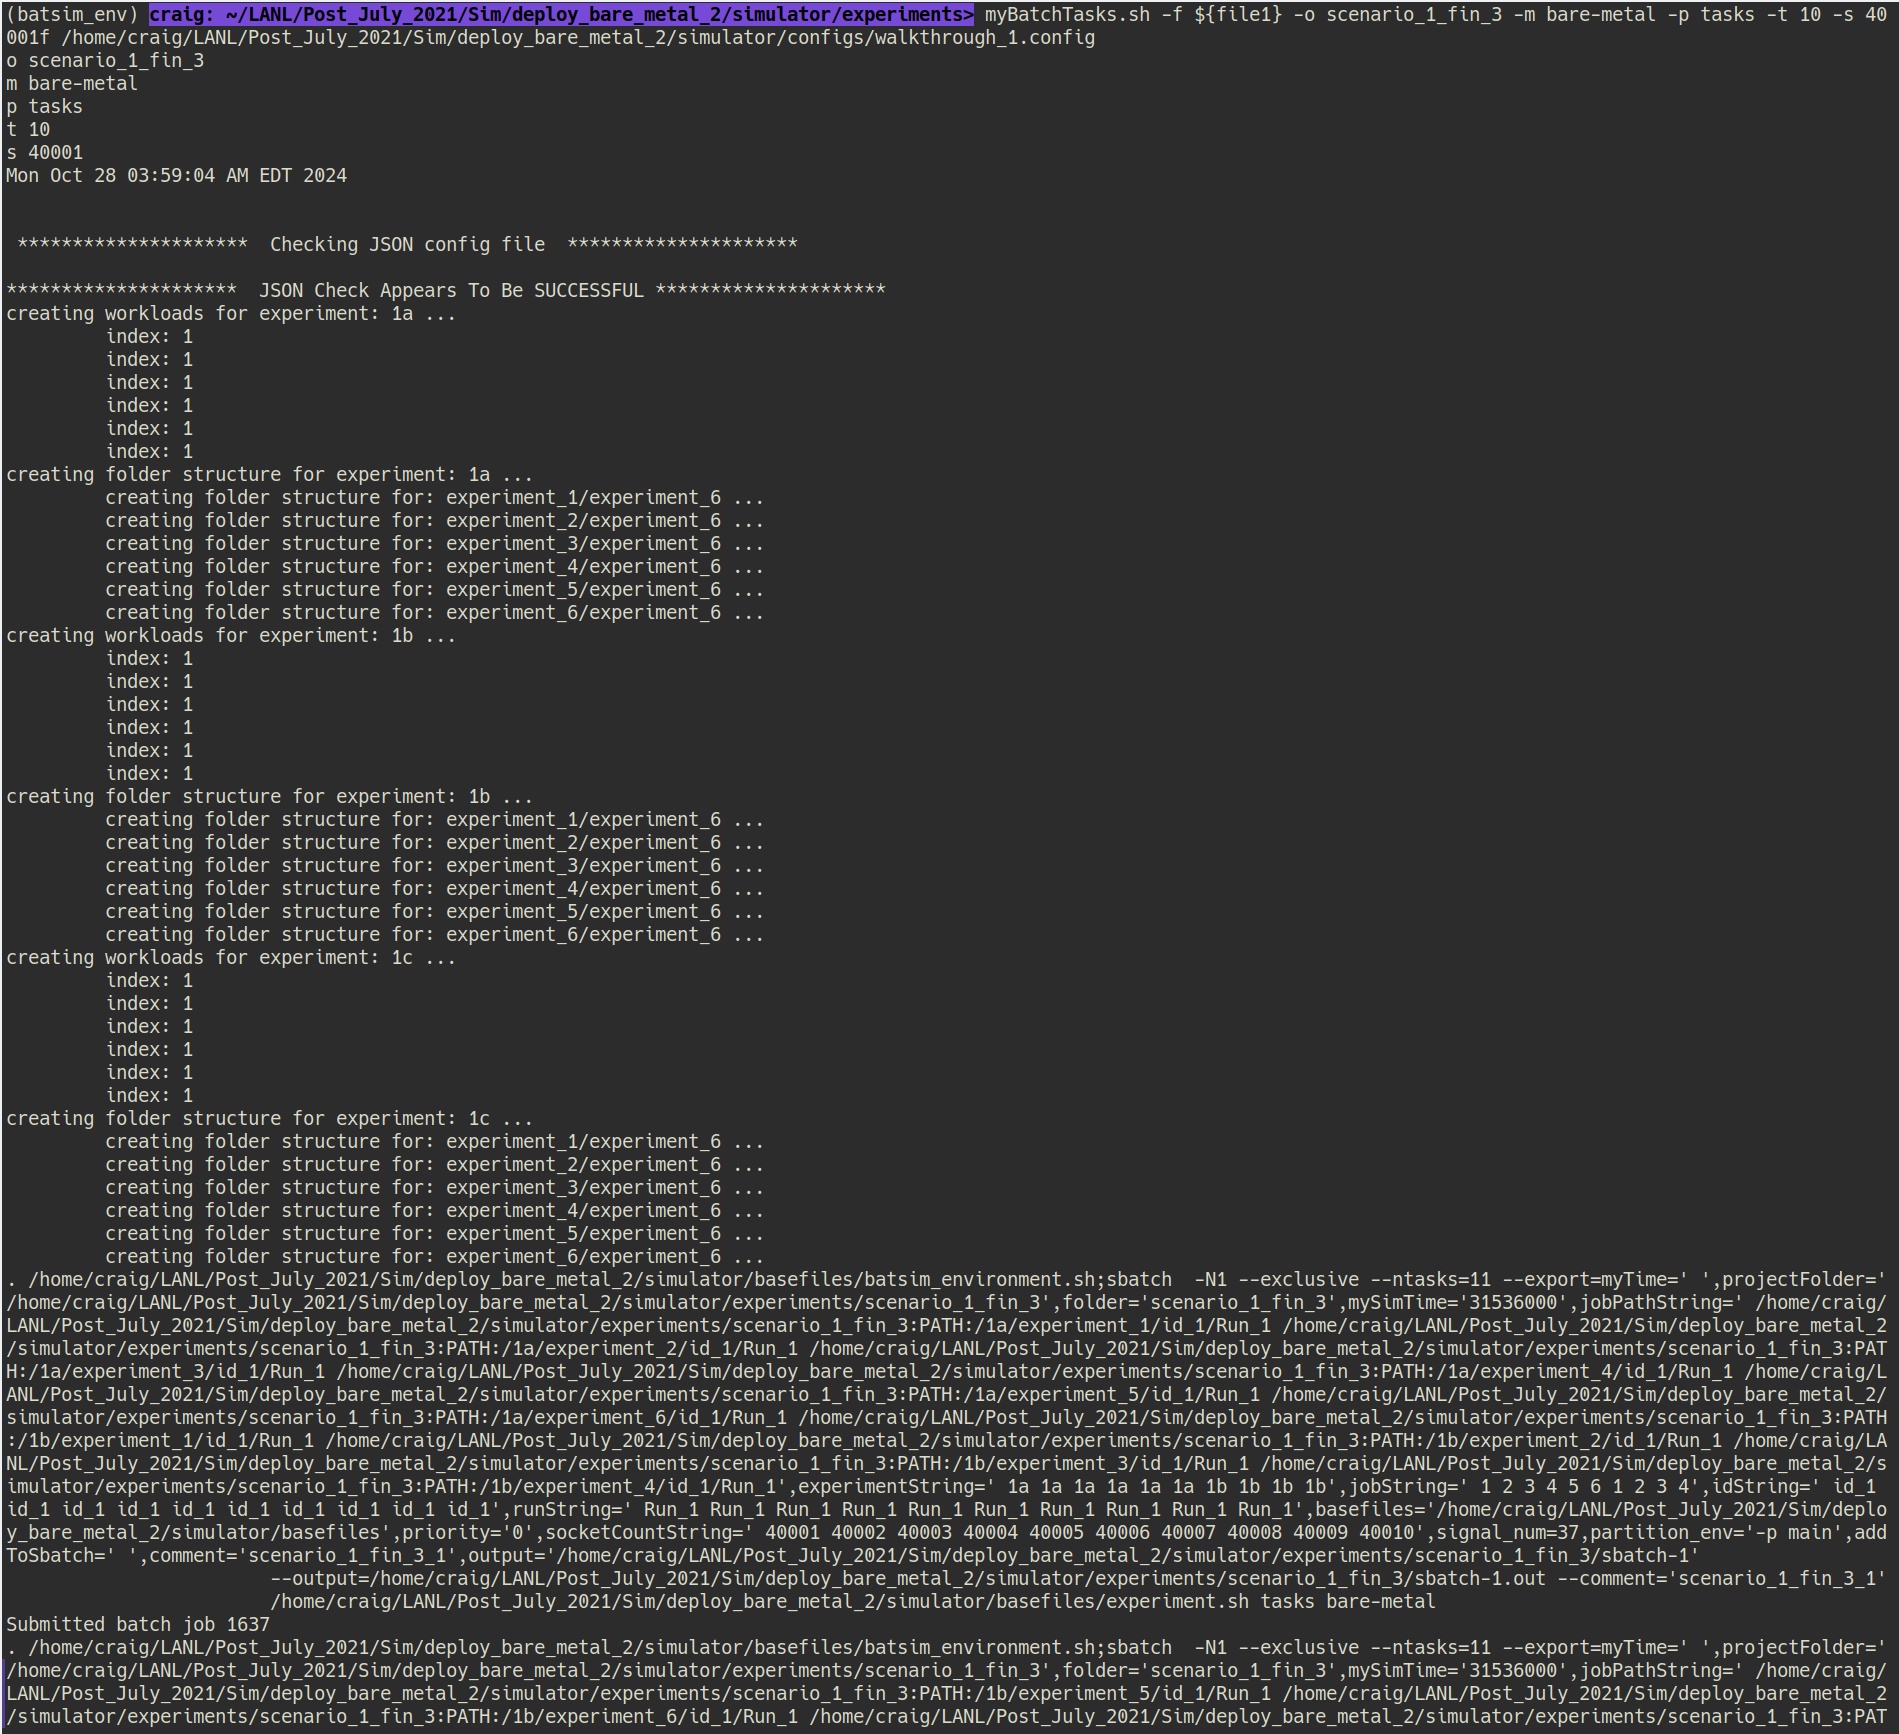
\includegraphics[scale=.5]{./scenario_1/myBatchTasks.png}

This shows first some debug info on what options were sent to the script.  Next comes a check
on the json included in the config file.  Next would normally come a workload filename that was
generated, but since we had already run this experiment the workload was already made with those
exact options so, for us, nothing needed to be generated.  You can see that for experiment 1a it made
sure that it had the workload it needed for each id, or just id\_1 in this case.

After that, it sets up the folder structure for the experiment and shows which job it is currently working on.
The time in between job folder set up can take a few minutes if you have a lot of runs, so don't get too worried if you don't see fast progress.

Next you will see a whole bunch of stuff dumped onto the screen.  This is the sbatch command that was used.  When you
are using \lstArg{-p "none"} or \lstArg{-p "background"} you will see something different.  But in this case,
you see that 2 batch jobs were submitted, one was numbered 1637, the other is cut-off but it is safe to assume 
it was 1638.

The next section details what to expect while running the sims.

\subsection{While Running The Sims}

\subsubsection{progress.sh}
While running the sims you can use our \lstTerm{progress.sh} script.  Of course you should definitely run \lstTerm{progress.sh --help},
but we will cover a couple options here and show you what to expect.

First let's show you a basic invocation of it.  While in the project folder, run \lstTerm{progress.sh -i $(pwd)}.
You should get something similar to the following:

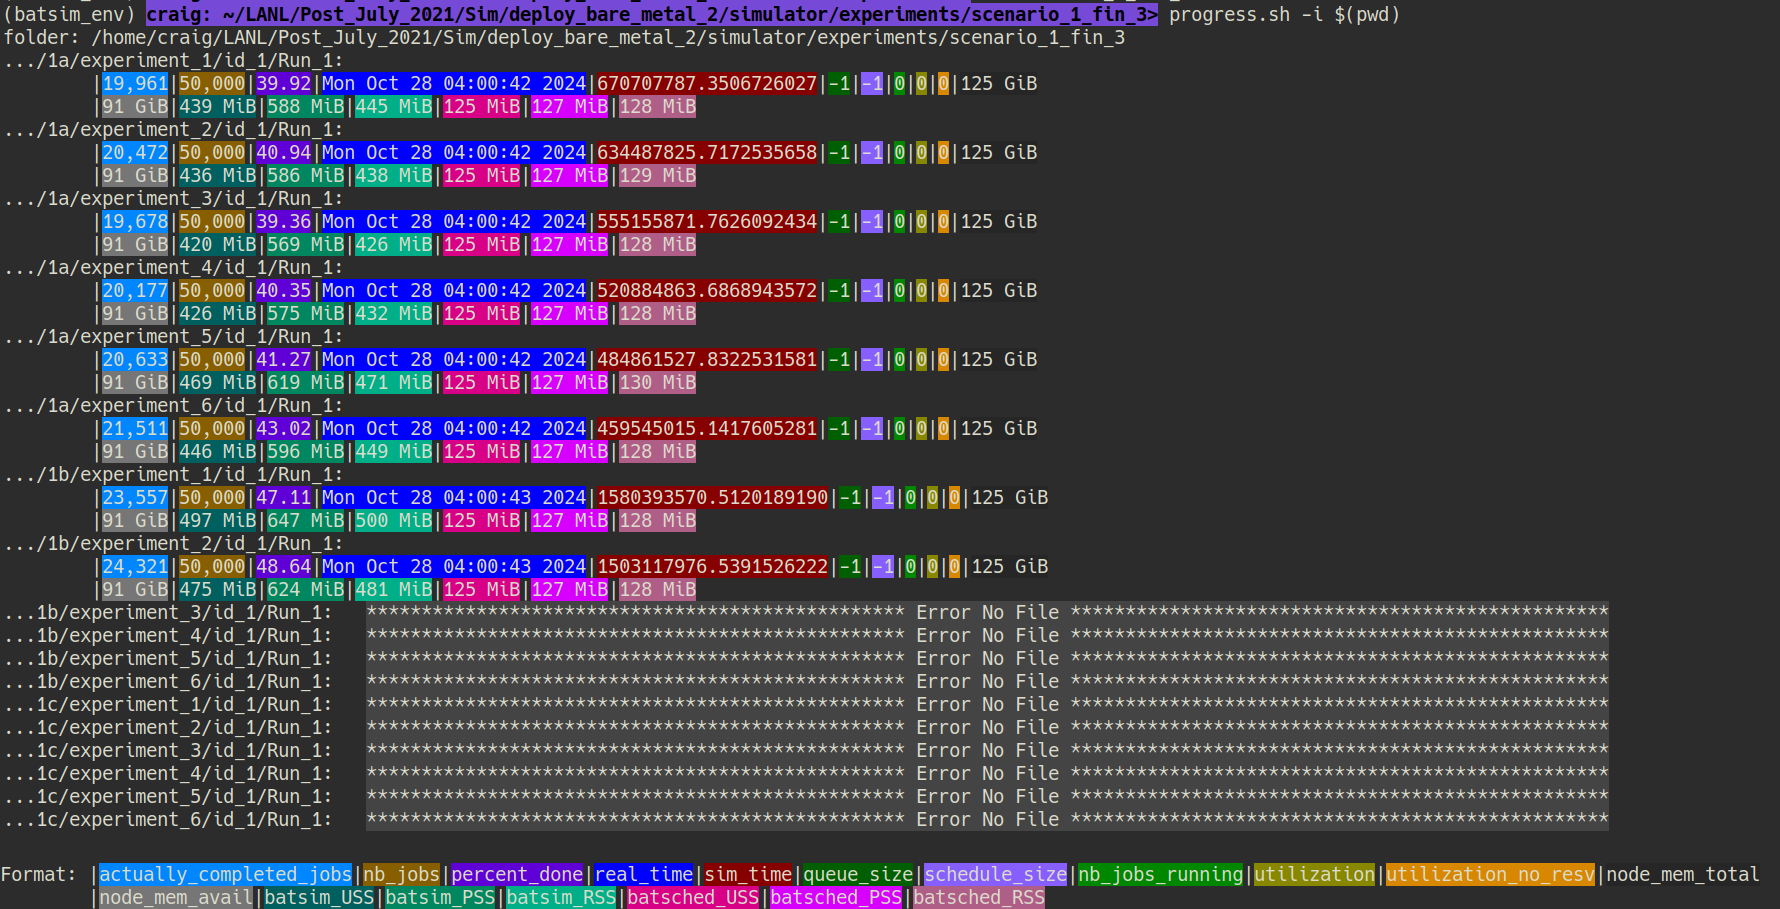
\includegraphics[scale=.4]{./scenario_1/progress_basic.png}

Notice with this view you get a lot of wasted space.  But it is easy for a beginner to see the correlation of the colors with what the colors and info
represent at the bottom.

You can hone in on the purple box as it is probably the most important as it tells what percent has completed so far.

Usually I recommend using the \lstArg{-Z} option, which will condense the space:

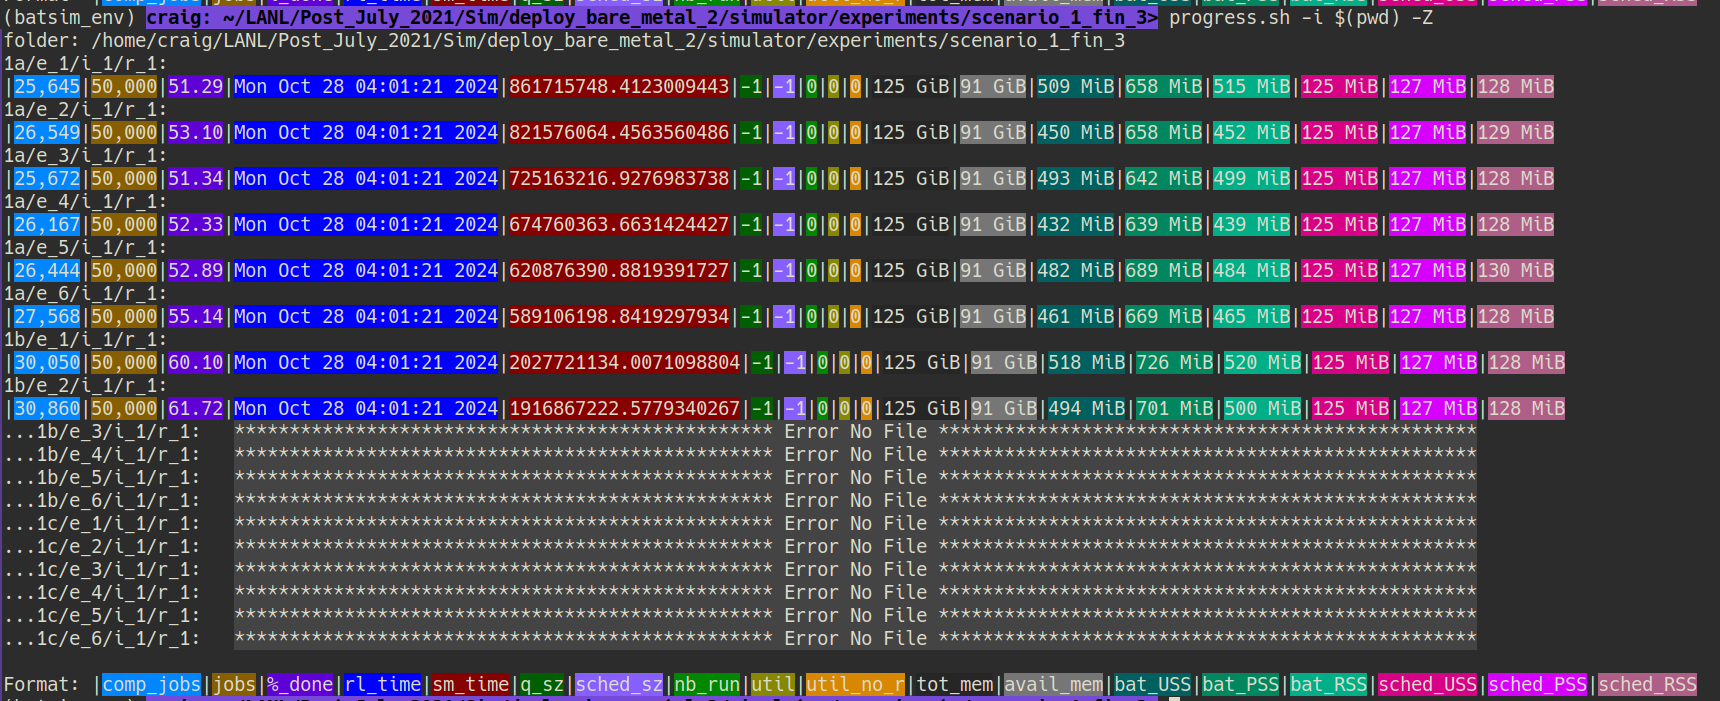
\includegraphics[scale=.4]{./scenario_1/progress_Z.png}

Notice the "Error No File" entries.  There could be many reasons for this, but in this instance it is simply that those
sims haven't started yet.

You can keep running the same command, using the up arrow, to see the progress.  \lstTerm{progress.sh}
allows for a lot of customization.
Suppose you don't want the memory being used shown.  You could tell it what you DO want shown and omit the memory, or
use the \lstArg{-z "m"} option.  \lstArg{-z} tells it what you DON'T want shown.

Here it is in action:

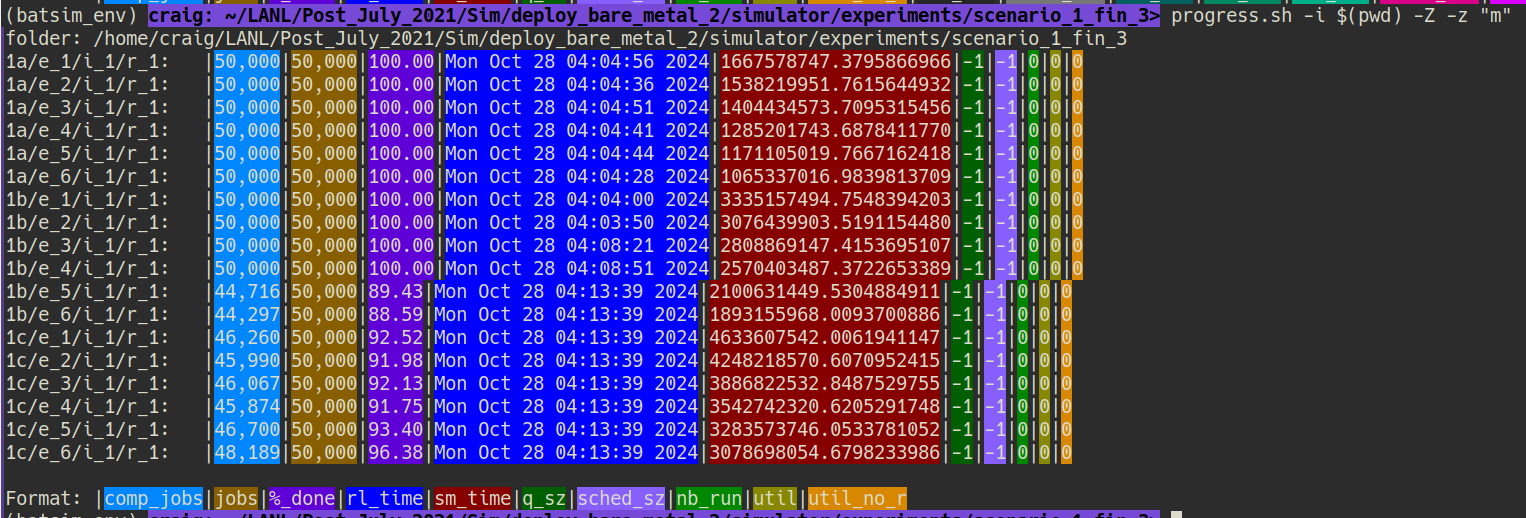
\includegraphics[scale=.4]{./scenario_1/progress_without_m.png}

You could also tell it you don't want the 'schedule info' at the same time, since this algorithm doesn't even use the schedule, by using \lstArg{-z "m S"}:

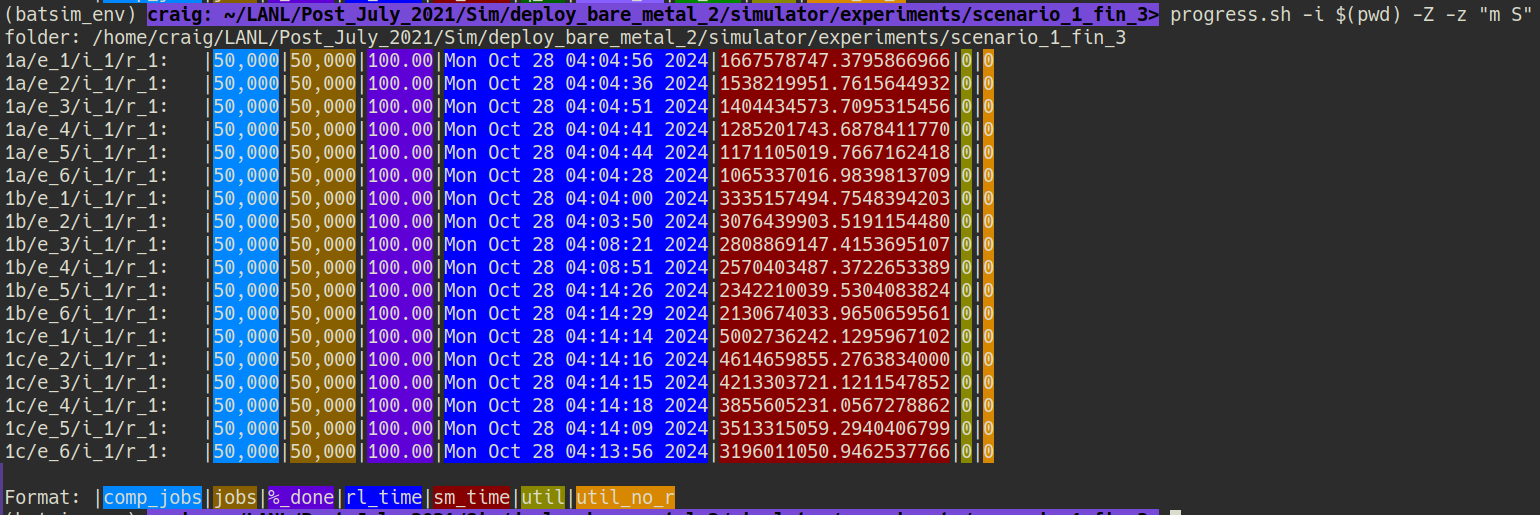
\includegraphics[scale=.4]{./scenario_1/progress_without_mS.png}

There is also an elapsed time you can show along with what not to show using the \lstArg{-E} option.

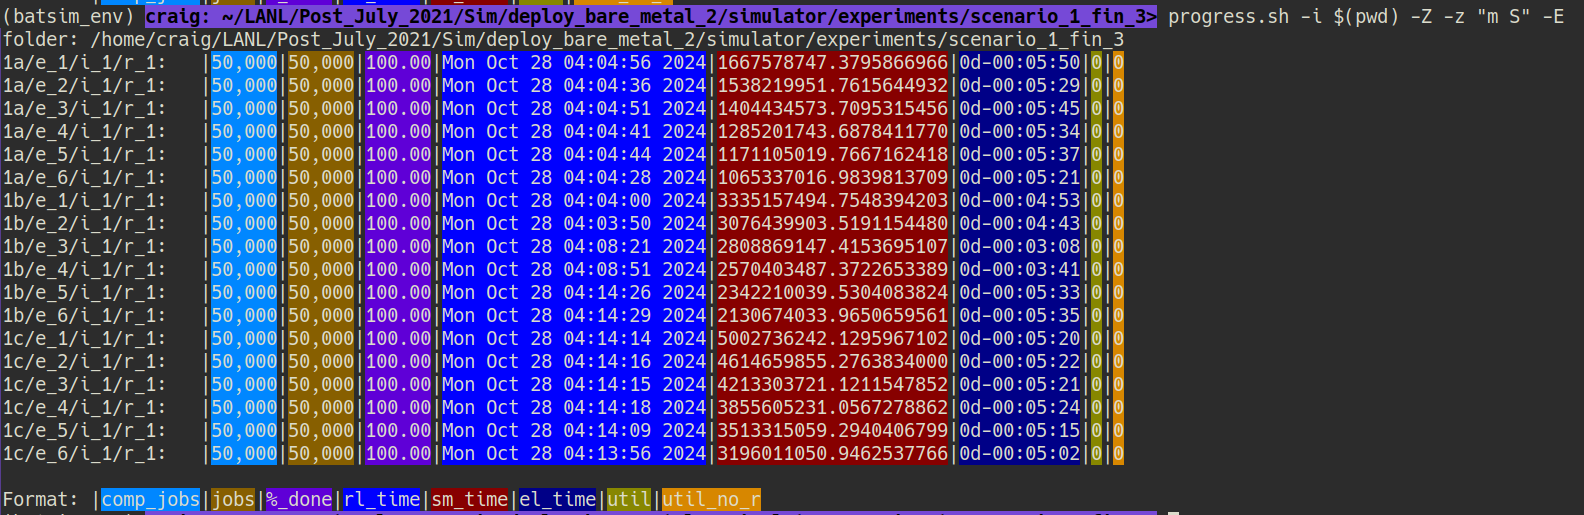
\includegraphics[scale=.4]{./scenario_1/progress_without_mS_E.png}

And finally, there is the \lstArg{-N} option which is more important when using real checkpointing which will be covered in Scenario 2:

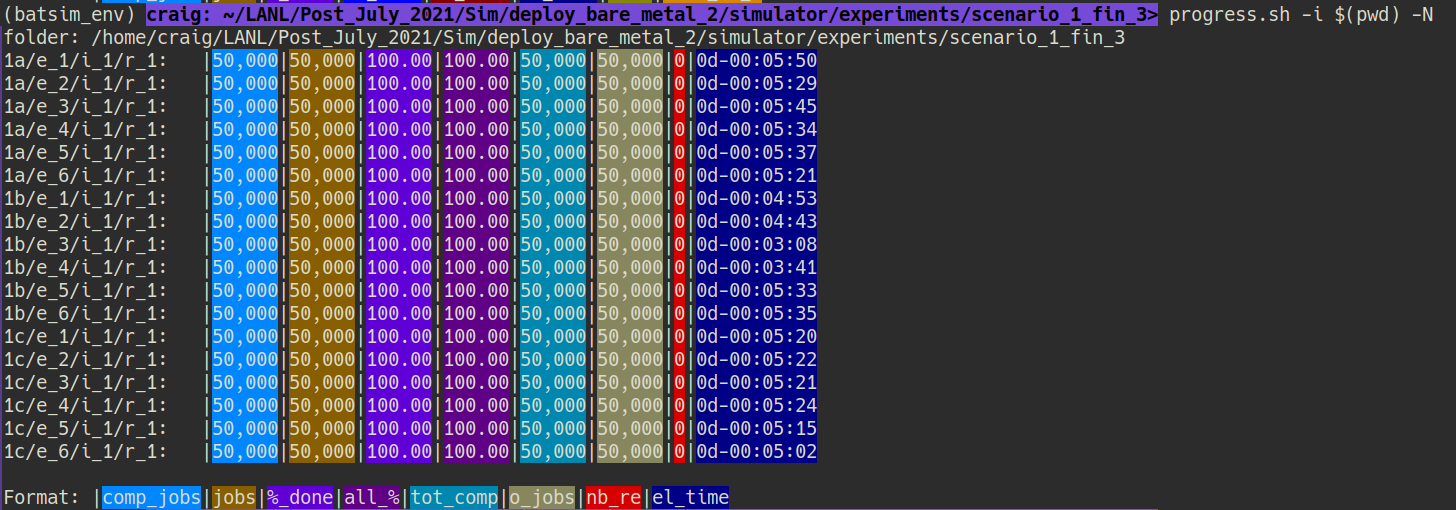
\includegraphics[scale=.4]{./scenario_1/progress_N.png}

There are many more options than that, but hopefully that gives you an idea of what to expect using \lstTerm{progress.sh}.

There are three more things to cover:
\begin{enumerate}
\item logs
\item srun output
\item sbatch output
\end{enumerate}

\subsubsection{logs}
So while you are running the sims we set the logging to \lstProperty{"batsim-log":"info"} and \lstProperty{"batsched-log":"CCU_DEBUG"}
for experiment "1a", so you can open these logs either while you are running the sims, or after.
\begin{warning}{Logs Can Get HUGE!!!}
Keep in mind that these logs can get very large depending on which verbosity you set.  This can cause the following problems:
@|
\begin{itemize}
\item sims become slow
\item no more storage to write out the logs, or anything for that matter, which will crash the sims
\item system crashes
\item when opening the logs it will take a long time to open, and may use all your memory depending on the text editor you choose.
\end{itemize}
@|
\end{warning}

The logs can be found in the \lstFolder{.../<Run Folder>/output/expe-out/log/} folder and there you will find:
\begin{itemize}
\item \lstFolder{sched.err.log}
\begin{itemize}
  \item where the batsched log goes.  This is usually what you want to look at.
\end{itemize}
\item \lstFolder{sched.out.log}
\begin{itemize}
  \item this is not used
\end{itemize}
\item \lstFolder{batsim.log}
\begin{itemize}
  \item where the batsim log goes.
\end{itemize}
\item \lstFolder{SoftErrors.log}
\begin{itemize}
  \item where the 'soft errors' go.  These are errors that might be useful, but don't impede the running of the sim.
\end{itemize}
\end{itemize}

Here is a look at the batsched log file:

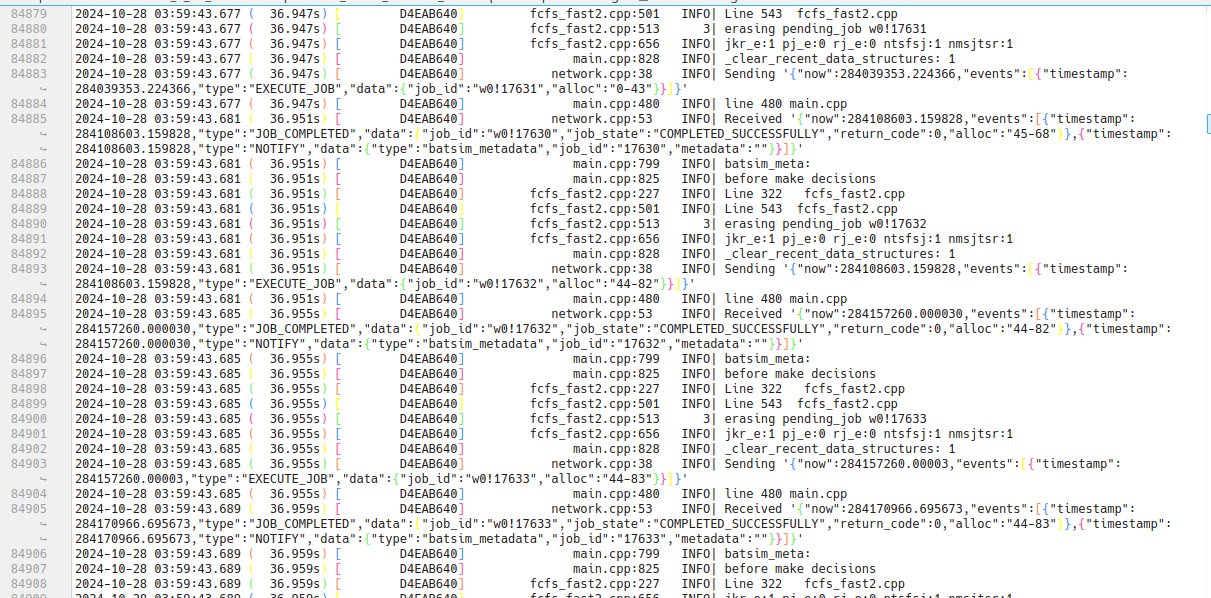
\includegraphics[scale=.6]{./scenario_1/log.png}

Notice on line 84883 you see the 'Sending' message.  This is where the scheduler is done for this pass and is sending info
over to Batsim.  Line 84885 has the scheduler coming alive again with a 'Received' message.  This back and forth messaging
will continue for the duration of the sim.

\subsubsection{srun output}

When using SLURM for parallelization, each srun execution will generate a \lstFolder{slurm-<jobid>.out} file in the \lstFolder{.../<Run folder>/output/} folder.
When using the real checkpointing this folder may have multiple \lstFolder{slurm-<jobid>.out} files, each
with their respective job id.

You can look at this file, or the \textit{latest} file in the case of real checkpointing, to see if any errors have happened.

\subsubsection{sbatch output}

When batches of files are being sent to SLURM, each sbatch gets its own output file.  This can tell us if something went wrong
at the sbatch level.  The files will be named \lstFolder{.../<project folder>/sbatch-<consecutive sbatch number>.out}.  When real checkpointing
is turned on and you have requeuing on then you will have \lstFolder{.../<project folder>-<consecutive sbatch number>_<resubmit number>.out} as a file.
This easily pollutes the project folder.  In the future, hopefully we can put these files in a folder of their own.






\subsection{Aggregating Results}
In order to aggregate results, we have a tool called \lstTerm{aggregate_makespan.py}.
To use, it is as simple as passing it the project folder:
\begin{termESC}
+?{prompt}+ cd /home/craig/simulator/experiments/Scenario_1
+?{prompt}+ aggregate_makespan.py -i $(pwd)     #  $(pwd) will give us the current directory
\end{termESC}

If you are running lots of runs, most of the time there will be a few simulations that don't complete for one reason or another.
You will see which ones didn't complete during aggregation. It will go job by job and tell you which ones did not complete
and then will total it up for you before going on to the next job.  A few aren't so bad, but a lot merits more investigation.

In order to save the results of the aggregation there is a file called \lstFolder{errors_total_makespan.txt}.  It has a summary at the bottom.
If everything went well with few, if any, sims not completing, then your aggregated results will be in \lstFolder{total_makespan.csv}

This brings us to the next step, of analyzing the \lstFolder{total_makespan.csv} file.
\subsection{Analysis}
Currently \lstFolder{total_makespan.csv} has the following header:

\csvreader[ %
tabular=|m{2.5cm}|m{2.5cm}|m{2.5cm}|m{2.5cm}|m{4cm}|m{3cm}|,
table head=\hline ,
late after line=\\\hline ]{tmh.csv}{}{\csvlinetotablerow}


We can then make the following code:
\begin{hicode}[python]
 
   
import pandas as pd
import numpy as np
import matplotlib.pyplot as plt
import seaborn as sns
fig, axs = plt.subplots(1, 1, figsize=(5, 5))

df = pd.read_csv("./total_makespan.csv",header=0,sep=",")

Adf=df.loc[df["exp"]=="1a"]
Bdf=df.loc[df["exp"]=="1b"]
Cdf=df.loc[df["exp"]=="1c"]

plt.plot(Adf["nodes"],Adf["makespan_sec"],label="1a")
plt.plot(Bdf["nodes"],Bdf["makespan_sec"],label="1b")
plt.plot(Cdf["nodes"],Cdf["makespan_sec"],label="1c")
plt.legend()
axs.set_xlabel("nodes")
axs.set_ylabel("makespan")
fig.suptitle("Scenario 1 -- Nodes VS Makespan")
fig.savefig("myplot.png",dpi=600)


  
  
\end{hicode}
\begin{center}
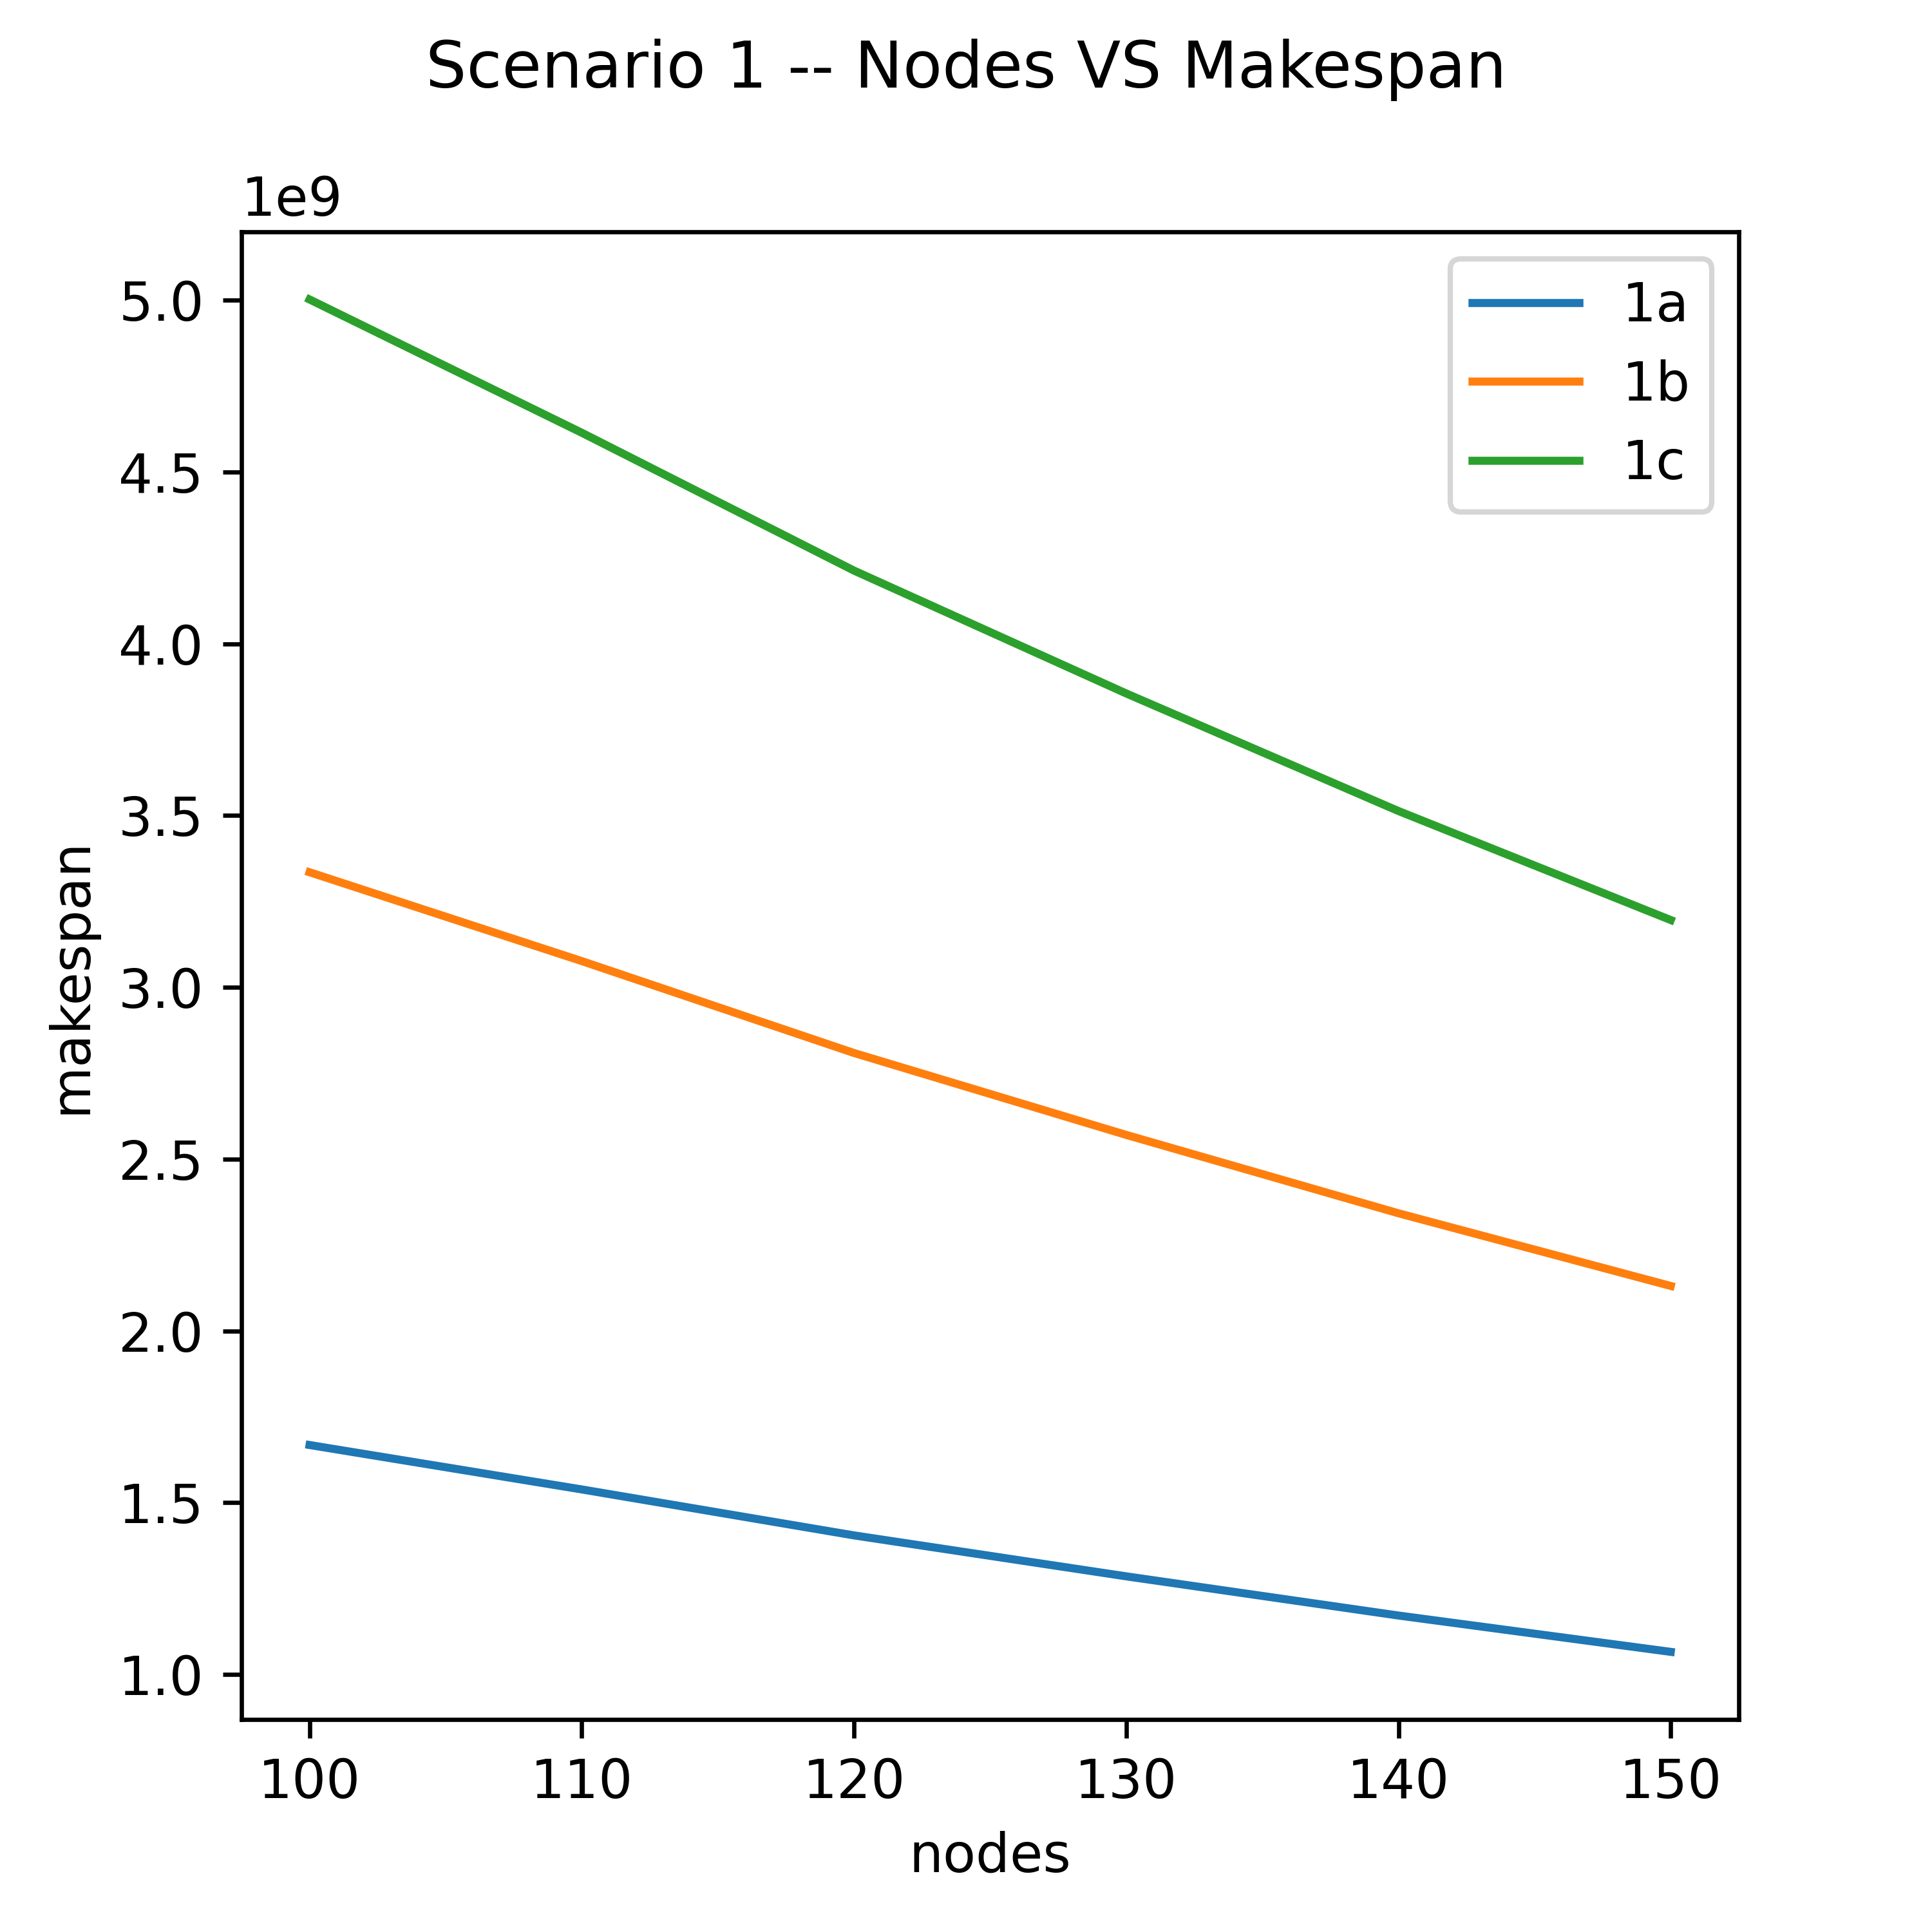
\includegraphics[scale=1.0]{./scenario_1/myplot.png}
\end{center}

\section{Scenario 2 - Easy Backfilling with Real Checkpointing}
\subsection{Scenario Description}
In this scenario we are going to use the easy\_bf3 algorithm.  It does easy backfilling without using the schedule.  We will use
this algorithm to show a miriad of things including:
\begin{itemize}
\item failures
\item repair times
\item real checkpointing
\begin{itemize}
  \item checkpoint signal
  \item automatic requeuing
  \item wallclock option
\end{itemize}
\item grizzly workload
\end{itemize}

We want to show that as repair time increases the avg-waiting time increases as well.  This would entice someone to
repair nodes sooner so that the quality of service is kept to a certain level.  The difference in the scenarios is that
Scenario 2a uses a fixed repair time sweep, whereas Scenario 2b uses a Mean Time To Repair sweep.

\begin{enumerate}
\item Scenario 2a
\begin{itemize}
  \item SMTBF: 16-64 by 16
  \item repairTime: 2-10 days by 2
  \item checkpoint interval: optimal
  \item queue-policy: ORIGINAL-FCFS
  \item real-checkpointing on: signal 37, automatic requeing, wallclock 6 minutes
  \item grizzly workload: 50,000 jobs , dump-time:3\%,read-time: 2\%
\end{itemize}
\item Scenario 2b
\begin{itemize}
  \item SMTBF: 16-64 by 16
  \item MTTR: 2-10 days by 2
  \item checkpoint interval: optimal
  \item queue-policy: ORIGINAL-FCFS
  \item real-checkpointing on: signal 37, automatic requeuing, wallclock 6 minutes
  \item grizzly workload: 50,000 jobs , dump-time:3\%,read-time: 2\%
\end{itemize}
\item Scenario 2c: Scenario 2a and 2b without SLURM, manual restart
\begin{itemize}
  \item SMTBF: 16-64 by 16
  \item MTTR: 2-10 days by 2
  \item checkpoint interval: optimal
  \item queue-policy: ORIGINAL-FCFS
  \item real-checkpointing on: interval every 4 minutes
  \item grizzly workload: 50,000 jobs , dump-time:3\%,read-time: 2\%
\end{itemize}
\end{enumerate}
\subsection{Make The Config File}
If you need a refresher on the format of a config file \hyperlink{general-config}{Scenario 1 covered that}.

Here we show what the config file we used looks like:
\begin{hicode}[java]
  {
    "2a":{
        "input":{
            "node-sweep":{
               "range":[1490]
            },
            "SMTBF-sweep":{
             "compute-SMTBF-from-NMTBF":true,
                "min":16,
                "max":64,
                "step":16,
                "formula":"1728000000*(1/i)"
            },
            "repairTime-sweep":{
                "min":2,
                "max":10,
                "step":2,
                "formula":"3600*24*i"
            },
            "checkpoint-sweep":{
                "range":["optimal"]
            },
            "batsched-policy":"easy_bf3",
            "checkpointing-on":true,
            "queue-policy":"ORIGINAL-FCFS",
            "seed-failures":10,
            "seed-failure-machine":10,
            "checkpoint-batsim-signal":37,
            "checkpoint-batsim-requeue":true,
            "start-from-checkpoint-keep":2,
            "grizzly-workload":{
                "type":"parallel_homogeneous",
                "machine-speed":1,
                "input":"sanitized_jobs.csv",
                "number-of-jobs":50000,
                "dump-time":"3%",
                "read-time":"2%",
                "time":"01-01-2018:"
            }

        },
        "output":{
            "avg-makespan":1

        }
    },
    "2b":{
        "input":{
            "node-sweep":{
               "range":[1490]
            },
            "SMTBF-sweep":{
             "compute-SMTBF-from-NMTBF":true,
                "min":16,
                "max":64,
                "step":16,
                "formula":"1728000000*(1/i)"
            },
            "MTTR-sweep":{
                "min":2,
                "max":10,
                "step":2,
                "formula":"3600*24*i"
            },
            "checkpoint-sweep":{
                "range":["optimal"]
            },
            "batsched-policy":"easy_bf3",
            "checkpointing-on":true,
            "queue-policy":"ORIGINAL-FCFS",
            "seed-failures":10,
            "seed-failure-machine":10,
            "seed-repair-times":10,
            "checkpoint-batsim-signal":37,
            "checkpoint-batsim-requeue":true,
            "start-from-checkpoint-keep":2,
            "grizzly-workload":{
                "type":"parallel_homogeneous",
                "machine-speed":1,
                "input":"sanitized_jobs.csv",
                "number-of-jobs":50000,
                "dump-time":"3%",
                "read-time":"2%",
                "time":"01-01-2018:"
            }

        },
        "output":{
            "avg-makespan":1

        }
    }
}

\end{hicode}

{\large \textbf{2a}}

So on line 4 we do the node-sweep but we just use a \lstProperty{"range"} with one value in it.  This is equivalent
to just setting the nodes to that number.  We use the sweep sometimes instead of setting the value outright just to keep
the syntax around for when we change the file.

Now on line 7 we do the SMTBF sweep.  We set \lstProperty{"compute-SMTBF-from-NMTBF":true} so that it will interpret
the values generated as NMTBF, but then convert them to the SMTBF based on each experiment's number of nodes.  We set the min, max, step starting on line 9.
We set a formula to operate on those generated numbers.  At Los Alamos National Lab, it was given to us that their biggest cluster "Trinity" had a NMTBF of 20k days.
We use this as a failure frequency but then increase it as we see fit.  In this case we are using 16x to 64x what Trinity supposedly has for a failure rate.

Line 14 starts our repair time sweep.  Repair time uses seconds so we do the math to convert to days using a formula.  So, we are doing
2-10 days with a step of 2 days.  On line 20 we set the simulated checkpoint interval to optimal (More to say about this in the 'Running the Config' section).

We then set the algorithm on line 23, and since we are using simulated checkpointing, we must turn it 'on' on line 24.  We set the queue-policy (for when a job is killed, where it goes in the queue)
to "ORIGINAL-FCFS".  We seed the failures, and the machine that failures choose to occur on.

We then do our real checkpointing options.  On line 28 we set \lstProperty{"checkpoint-batsim-signal":37} so that SLURM will send a signal 37 to
the sims to tell it to do a real checkpoint when a certain amount of time is left before the wallclock time is done.  This setting is set in the \lstFolder{batsim_environment.sh} file.
If we do the following:

\begin{termESC}
+?{batprompt}+ cd $basefiles_prefix
+?{batprompt}+ cat batsim_environment.sh

#############################################################################
# Edit prefix before doing anything, this is mandatory
#
# Here you will find some SBATCH variables you can set
# All SBATCH variables can be set here, not just the ones
# included.  And of course uncomment the line to take effect.
# ALL SBATCH variables can be found here:
# 
#
# This file can be edited after ./myBatchTasks.sh
# finishes for another batch of simulations with different
# parameters.  Just make sure you keep up with socket-start
# so no sims are overlapping with socket numbers
#############################################################################




export prefix="/home/craig/LANL/Post_July_2021/Sim/deploy_bare_metal_2/simulator"

export SBATCH_PARTITION=main
#export SBATCH_QOS=standard
#export SBATCH_NO_REQUEUE="yes"
+?{textbf}{?{color}{red}export SBATCH?{underscore}SIGNAL=?{quotes}B:37@120?{quotes}}  {?{color}{myTerminalRed} <----------------------  here}+


export basefiles_prefix=$prefix/basefiles
export install_prefix=$prefix/Install
export downloads_prefix=$prefix/Downloads
export python_prefix=$prefix/python_env

export PATH=$PATH:$prefix/charliecloud/charliecloud/bin:$basefiles_prefix:\
       $basefiles_prefix/tests:$basefiles_prefix/debug_files:$prefix:\
       $install_prefix/bin:/usr/bin:/usr/sbin
export LD_LIBRARY_PATH=$LD_LIBRARY_PATH:$install_prefix/lib:$install_prefix/lib64
export LMOD_SH_DBG_ON=1
source $python_prefix/bin/activate
source $basefiles_prefix/helpful_functions.sh

\end{termESC}
you can see on line 27 that we set signal 37 to 120 seconds before the wallclock time ends. The 120 seconds will need adjusting 
based on how long it takes to write out your checkpoint.  But that's what \lstTerm{37@120} means.
As far as the \lstTerm{B:}, that tells it to send the signal to the sbatch script and not the individual steps.  That is needed
in our setup and was changed to require this when we added the automatic requeuing.

Ok, back to the config file:
On line 29 we tell it we want to requeue automatically if the walltime is insufficient to complete the sim.  And on line
30 we get the \lstProperty{"start-from-checkpoint-keep":2}.  This says that since we are requeuing automatically we will be starting from
a checkpoint, possibly multiple times, and we want to keep the 'Frames' before the current one.  Look at the User\_Doc\_Manual.pdf
{\textbf{\color{blue}Section 1.3.7:}\color{blue}\hspace{1mm}Real Checkpointing: checkpoint\_\#/ and expe-out\_\#/}

On line 31 we make a grizzly workload and tell it what file to use for the workload.  The 2018 real grizzly data is the "sanitized\_jobs.csv" file.
We are going to start at the beginning of the year of 2018, but we only want 50k jobs so we set that on line 35.

On line 36 and 37 we set the \lstProperty{"dump-time":"3%"} and \lstProperty{"read-time":"2%"}.  This is required if you
are going to use simulated checkpointing.  And on line 38 we say we want to start the jobs at the beginning of 2018 and go to the latest date of the file.
We are talking about the times the jobs were submitted when we are talking about this \lstProperty{"time":} property.

{\large \textbf{2b}}

The only difference here is that we use a MTTR (Mean Time To Repair) sweep on line 59 instead of the repairTime sweep we used on line 14.
\subsection{Run The Config File}
First off, we all make mistakes, so when I went to run this config file I got an error with line 24.  I will show you this error
so you don't panic when you see it.  It is very common to get your config in improper json.

So let's see the output:

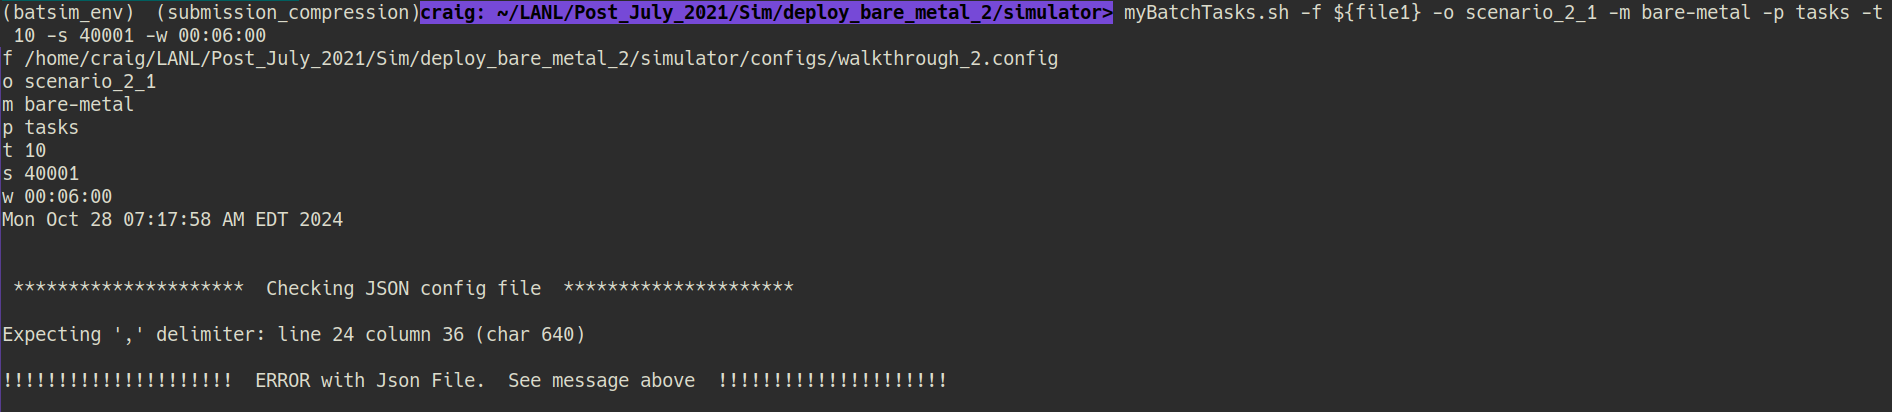
\includegraphics[scale=.5]{./scenario_2/json_error.png}

So I forgot to use a ',' is what it told me.  What the case actually was - was that I put double quotes on the right side of \lstProperty{"checkpointing-on":true",}.
See the mistake?  'true' shouldn't be quoted as it is recognized as a bool, but not only that, I only had the quote on the right side. 

Now, in running this config, I had made another mistake and didn't add in the \lstProperty{"dump-time":} or \lstProperty{"read-time":} properties
for the grizzly workload the first time around.  Since I was using simulated checkpointing, this was required.

So having this error started a bunch of simulations, but when I looked at their progress using \lstTerm{progress.sh}, all of the sims
were showing "Error No File".  This can happen early in the sim as it may take time for a job to finish, which is what populates the progress info.
But alas, a couple minutes went by and I could tell something was up.  So I looked at the first experiment: "2a" and the first job: "experiment\_1" and went to:
\lstFolder{id_1/Run_1/output/slurm-<jobid>.out} and looked at that file.  It showed me the following:

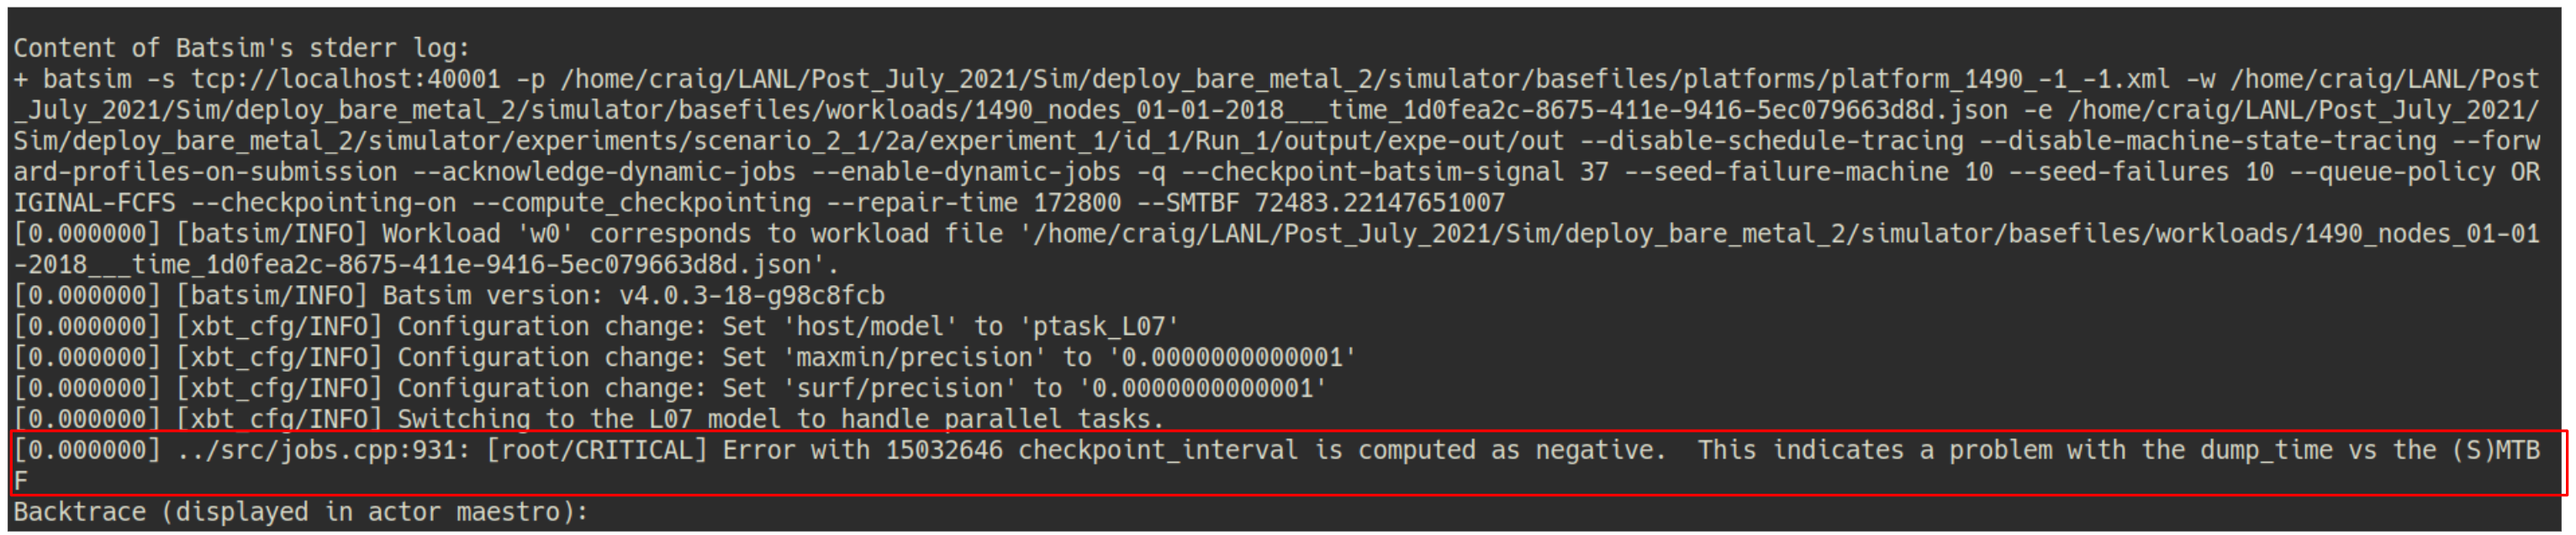
\includegraphics[scale=.25]{./scenario_2/sim_error.png}

The error at first sounds terrible.  But I am familiar with this.  When calculating the checkpoint interval, and especially an optimal checkpoint, the SMTBF needs
to be known as well as the dump and read times.  I forgot to add them to the workload description in the config file.  Once I did that everything worked as planned.

Before I ran the command, however, I used my trusty \lstTerm{batEdit} command to edit the config file:

\begin{termESC}
+?{batprompt}+ batEdit -e -o "-ltr"
\end{termESC}

This showed the following:

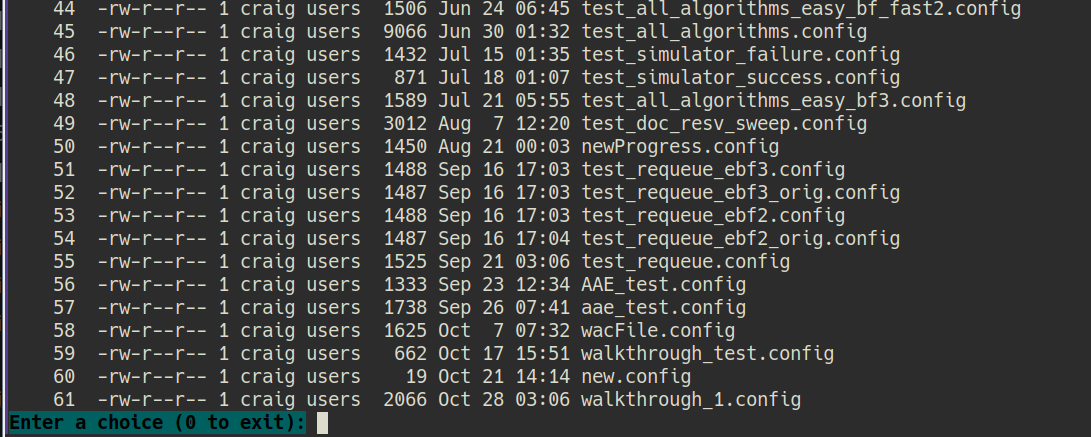
\includegraphics[scale=.5]{./scenario_2/batEdit.png}

So I wanted to edit walkthrough\_1.config so I typed: '61'  as a choice (no quotes).
Scenario 2 was much different than Scenario 1 so I simply did a Ctrl+6 to mark the text, used page-down to go to the bottom of the file
and hit Ctrl+k to cut the text.  Then I copied and pasted what you see in this pdf file for Scenario 2's config.
Ctrl+o to save, but I made sure to save it to 'walkthrough\_2.config', Ctrl+x to exit.

One last step.  We saved to a different file than we chose using batEdit.
Run it again and choose our new file:
\begin{termESC}
+?{batprompt}+ batEdit -o "-ltr"
\end{termESC}

This time we are not editing the file, we just want to choose it.

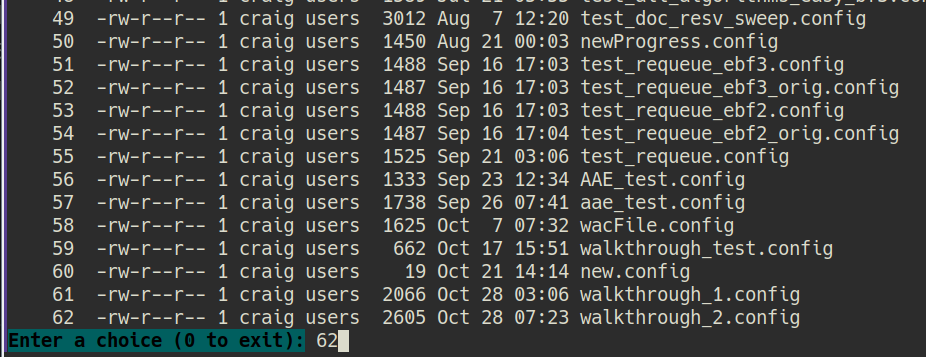
\includegraphics[scale=.5]{./scenario_2/batEdit_2.png}

And here is the command I used to run it.

\begin{termESC}
+?{batprompt}+ myBatchTasks.sh -f ${file1} -o scenario_2_1 -m bare-metal -p tasks -t 10 -s 40001 -w 00:06:00
\end{termESC}

It is a lot like before except we added on \lstArg{-w 00:06:00}.  This is the wallclock time.  It tells SLURM that our sbatch
script should only take 6 minutes.  And as you know from our \lstFolder{batsim_environment.sh} file, we send signal 37 at 120 seconds before
the wallclock is going to be reached.  So in this case, after running 4 minutes, we are going to do a real checkpoint and respawn the jobs.

\subsection{While Running The Sims}

\subsubsection{progress.sh}

So we covered a lot of basic options for \lstTerm{progress.sh} in Scenario 1.  What is important in this Scenario is to show
the resubmission elements.

So here are the sims just starting.  Notice I use \lstTerm{progress.sh -i $(pwd) -N -e "2a" }.  The \lstArg{-N} option gets me
most of what I want for looking at resubmitted jobs and the \lstArg{-e "2a"} shows just experiment "2a" which cuts down on how much we see.

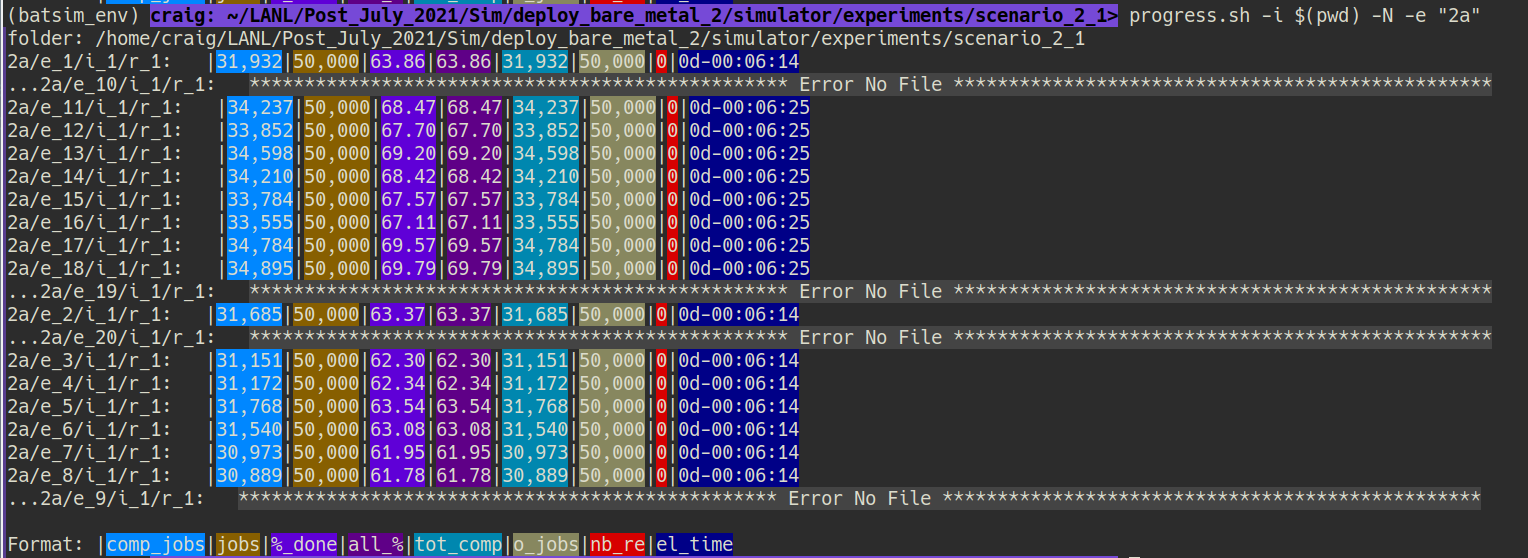
\includegraphics[scale=.5]{./scenario_2/progress_2a.png}

Some things to mention:  The completed jobs and the total completed are the same number in resubmit 0.  That red column is the resubmit number.
The jobs and original jobs are the same number as well, and the percent done and overall percent done, they are all the same numbers.

So lets look a little later after the jobs have respawned and have been queued in SLURM and have now moved into the RUNNING state.

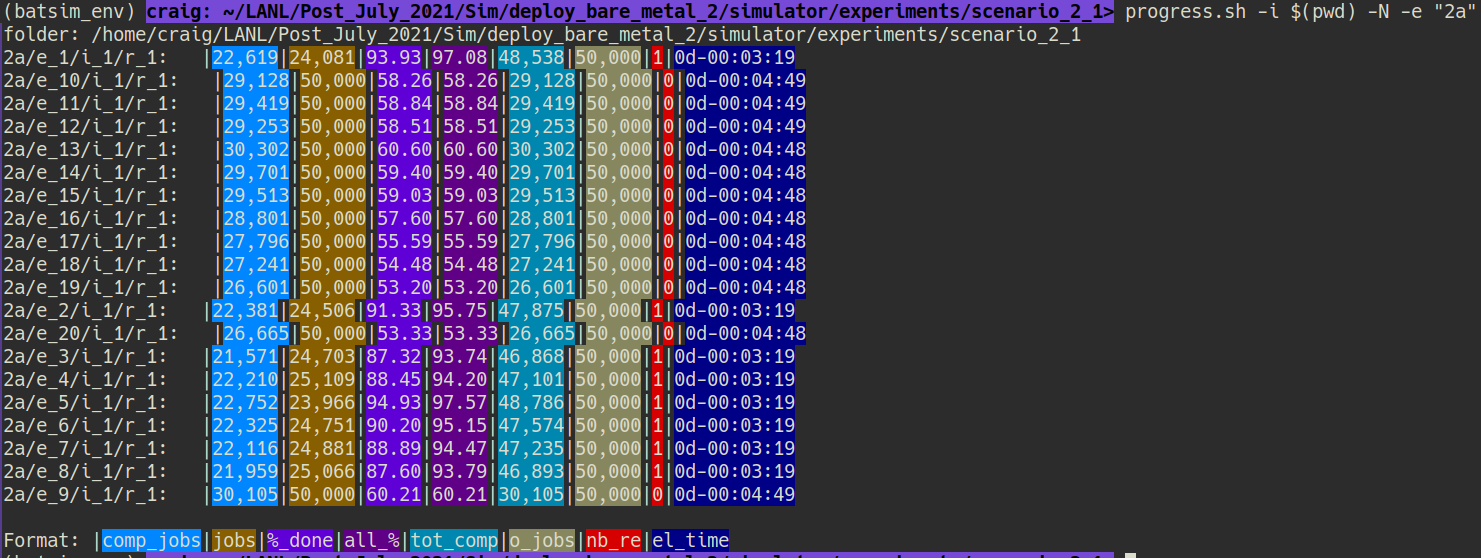
\includegraphics[scale=.5]{./scenario_2/progress_nb_re_1.png}

Now you see a difference for the jobs that have a nb\_resubmit of 1.  The overall percent is different than the \%\_done.  The jobs is different
than the original\_jobs and the completed\_jobs is different than total\_completed.

And finally you can see that all of them are completed:

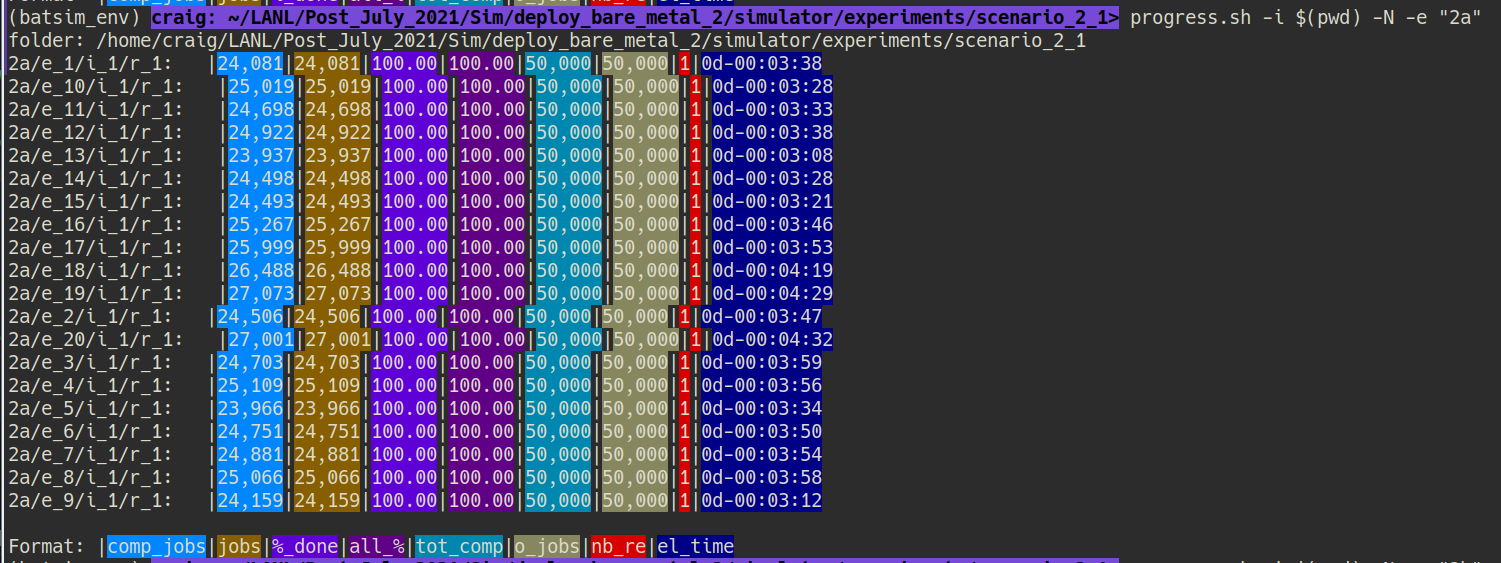
\includegraphics[scale=.5]{./scenario_2/progress_completed.png}

\subsubsection{Checkpointing Folders}
Now that everything is finished, you can see the folder structure that has been left:

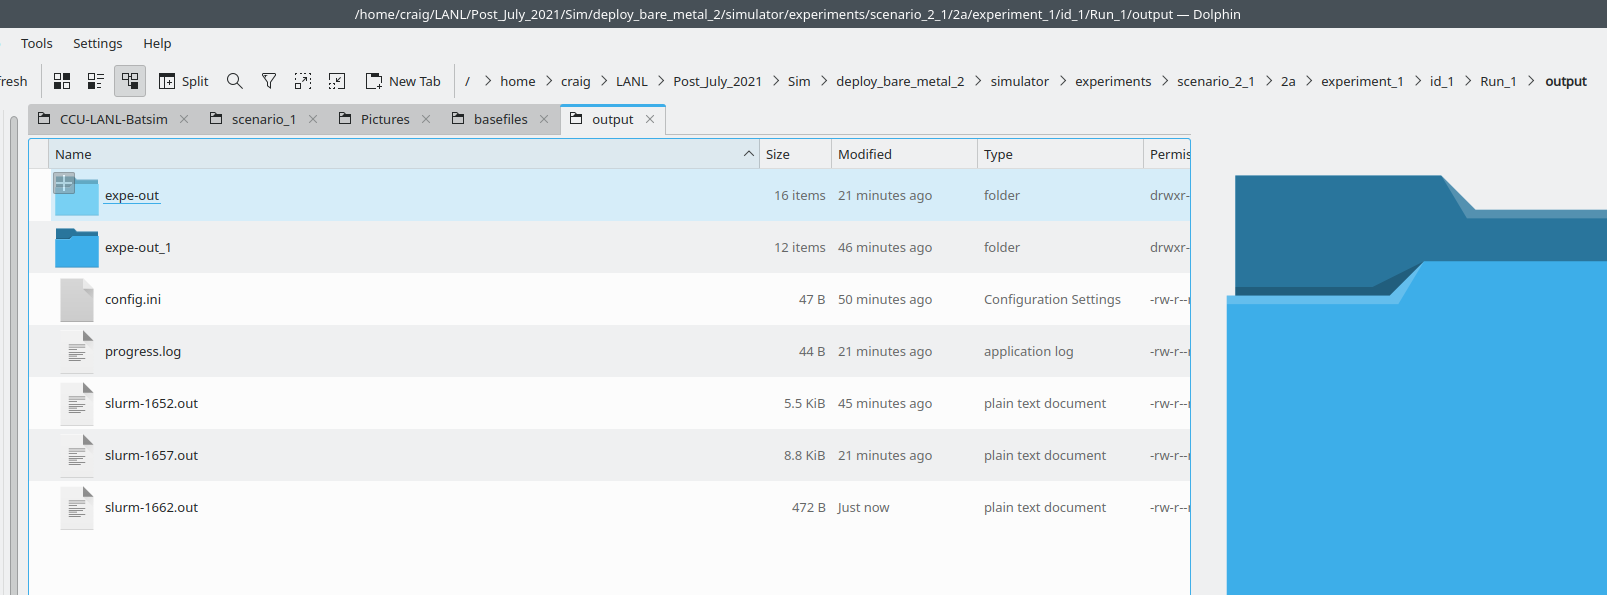
\includegraphics[scale=.47]{./scenario_2/output.png}

Here you can see that since we kept a max of 2 'Frames' and there was only 1 resubmit, that there is
only one \lstFolder{.../output/expe-out_#} and that folder is \lstFolder{.../output/expe-out_1}.

If there had been more resubmits, there would be an \lstFolder{.../output/expe-out_2}, but since we only said
to keep 2, that would be the highest the 'Frames' would go to.

Let's look into \lstFolder{expe-out_1}

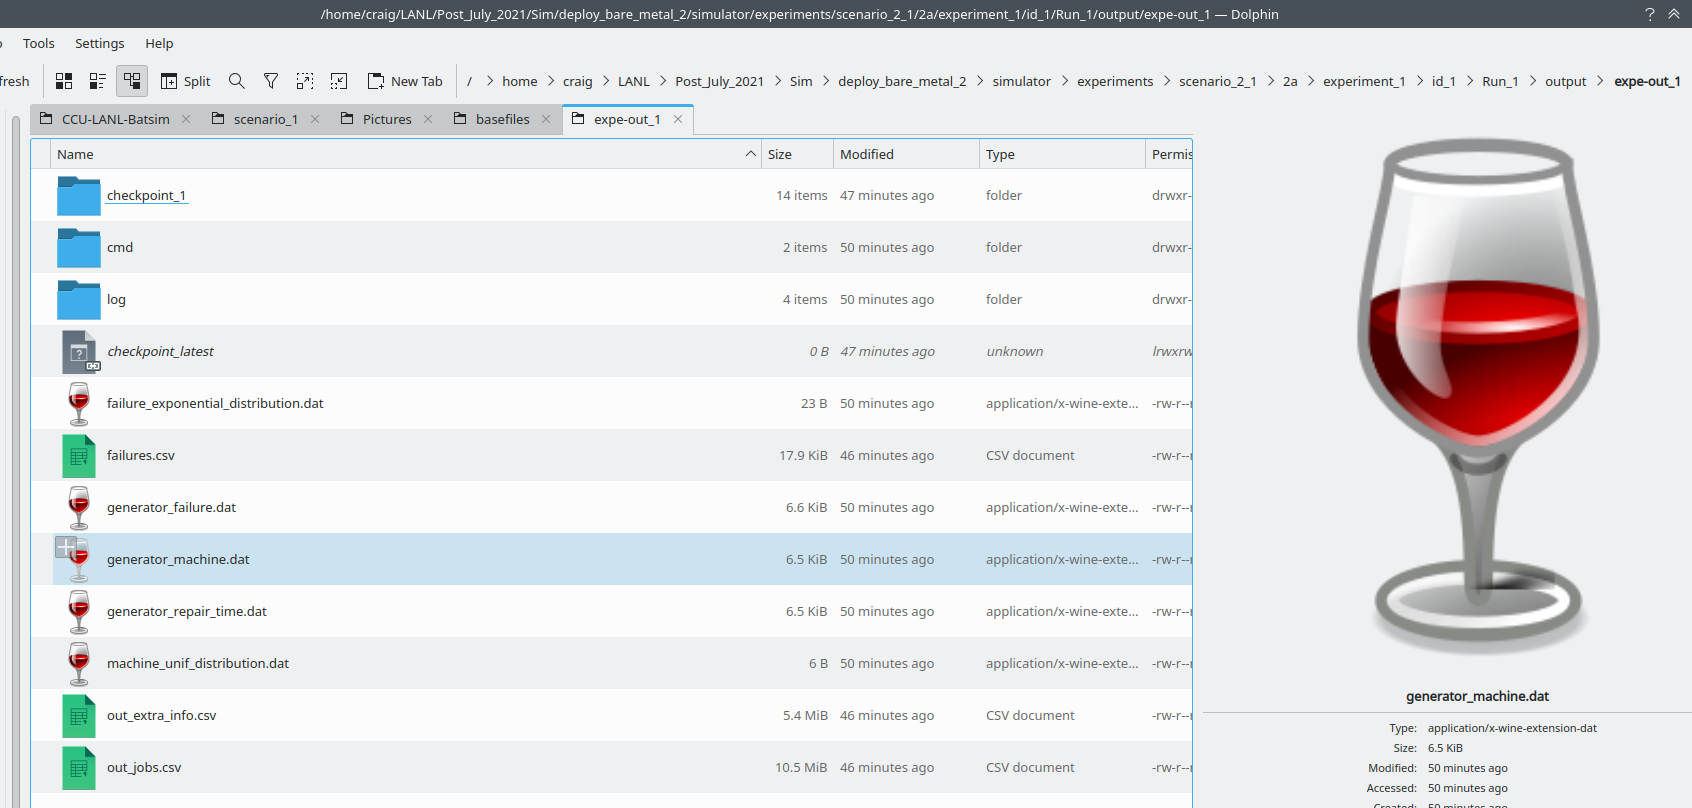
\includegraphics[scale=.45]{./scenario_2/expe-out_1.png}

We can see that a single checkpoint did occur in this older 'Frame'.

Now lets go back up a folder and peek into \lstFolder{.../output/expe-out/}

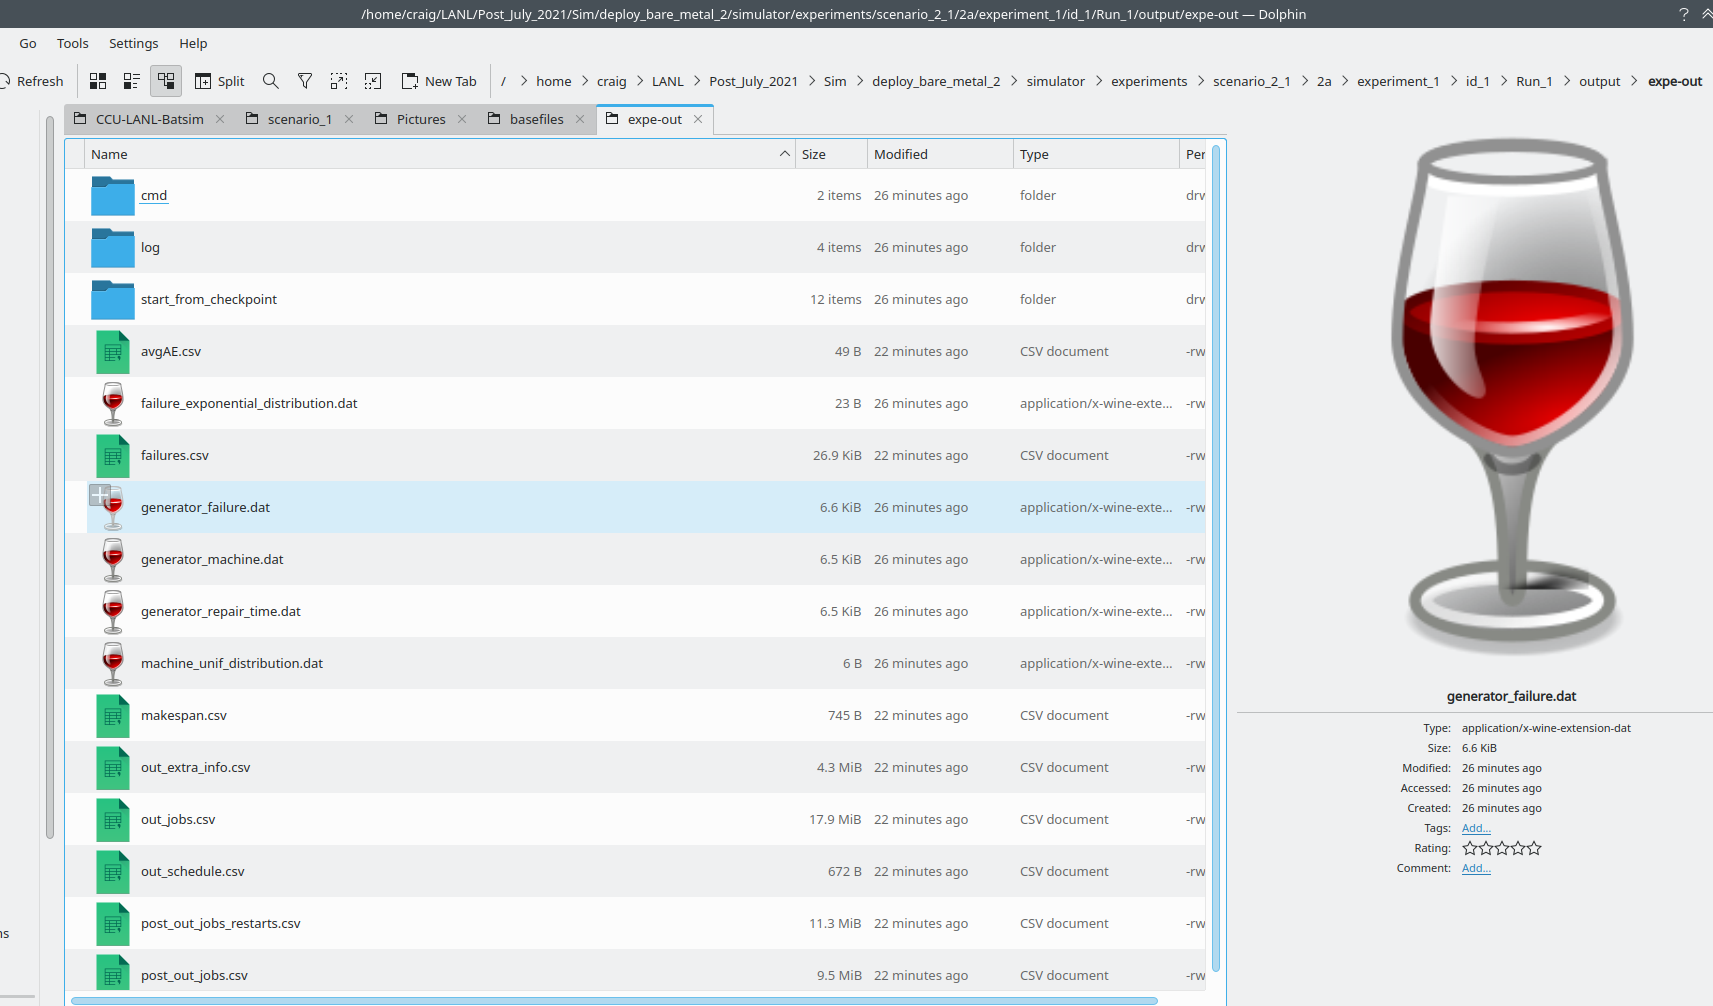
\includegraphics[scale=.45]{./scenario_2/expe-out.png}

You can see here that this 'Frame' started from a checkpoint given the folder: \lstFolder{.../output/expe-out/start_from_checkpoint}.
You also DON'T see a \lstFolder{checkpoint_1} folder since it didn't need to checkpoint.  You do see a \lstFolder{makespan.csv} file, which
tells us everything finished on this sim.




\subsection{Aggregating Results}
So now we aggregate the results like normal:

\begin{termESC}
  +?{batprompt}+ cd ${prefix}/experiments/scenario_2_1
  +?{batprompt}+ aggregate_makespan.py -i $(pwd)
\end{termESC}

\subsection{Analysis}
Currently \lstFolder{total_makespan.csv} has the following header:

\csvreader[ %
tabular=|m{2.5cm}|m{2.5cm}|m{2.5cm}|m{2.5cm}|m{4cm}|m{3cm}|,
table head=\hline ,
late after line=\\\hline ]{tmh.csv}{}{\csvlinetotablerow}

We can then make the following code:
\begin{hicode}[python]
 
  import pandas as pd
  import numpy as np
  import matplotlib.pyplot as plt
  import seaborn as sns
  
  width=5
  height=5
  BASE_SECONDS = 1728000000
  
  fig, axs = plt.subplots(1, 1, figsize=(width, height))
  
  df = pd.read_csv("./total_makespan.csv",header=0,sep=",")
  #change NMTBF to be normalized to BASE_SECONDS.  Example 1x,2x,...,32x
  df.loc[:,"NMTBF"]=BASE_SECONDS / df["NMTBF"]
  
  #get a list of failure rates and sort in reverse
  NMTBF_times = list(df["NMTBF"].unique())
  NMTBF_times.sort(reverse=True)
  
  Adf=df.loc[df["exp"]=="2a"]
  Bdf=df.loc[df["exp"]=="2b"]
  
  
  current_df=Adf
  for nmtbf in NMTBF_times:
      nmtbf_df=current_df.loc[current_df["NMTBF"]==nmtbf]
      plt.plot(nmtbf_df["repair-time"],nmtbf_df["avg_waiting"],label=f"{int(nmtbf)}x")
  plt.legend()
  axs.set_xlabel("repair time(days)")
  axs.set_ylabel("avg waiting time")
  ticks=list(range(3600*24*2,3600*24*12,3600*24*2))
  labels=[f"{i}days" for i in range(2,12,2)]
  axs.set_xticks(ticks)
  axs.set_xticklabels(labels,rotation=45)
  fig.suptitle("Scenario 2a -- repair time VS avg waiting time using fixed repair time")
  fig.savefig("myplot.png",dpi=600)
  
  fig, axs = plt.subplots(1, 1, figsize=(width, height))
  current_df=Bdf
  for nmtbf in NMTBF_times:
      nmtbf_df=current_df.loc[current_df["NMTBF"]==nmtbf]
      plt.plot(nmtbf_df["MTTR"],nmtbf_df["avg_waiting"],label=f"{int(nmtbf)}x")
  plt.legend()
  axs.set_xlabel("repair time(days)")
  axs.set_ylabel("avg waiting time")
  ticks=list(range(3600*24*2,3600*24*12,3600*24*2))
  labels=[f"{i}days" for i in range(2,12,2)]
  axs.set_xticks(ticks)
  axs.set_xticklabels(labels,rotation=45)
  fig.suptitle("Scenario 2b -- repair time VS avg waiting time using MTTR")
  fig.savefig("myplot2.png",dpi=600)
  
    
\end{hicode}
And here are the results:
\begin{center}
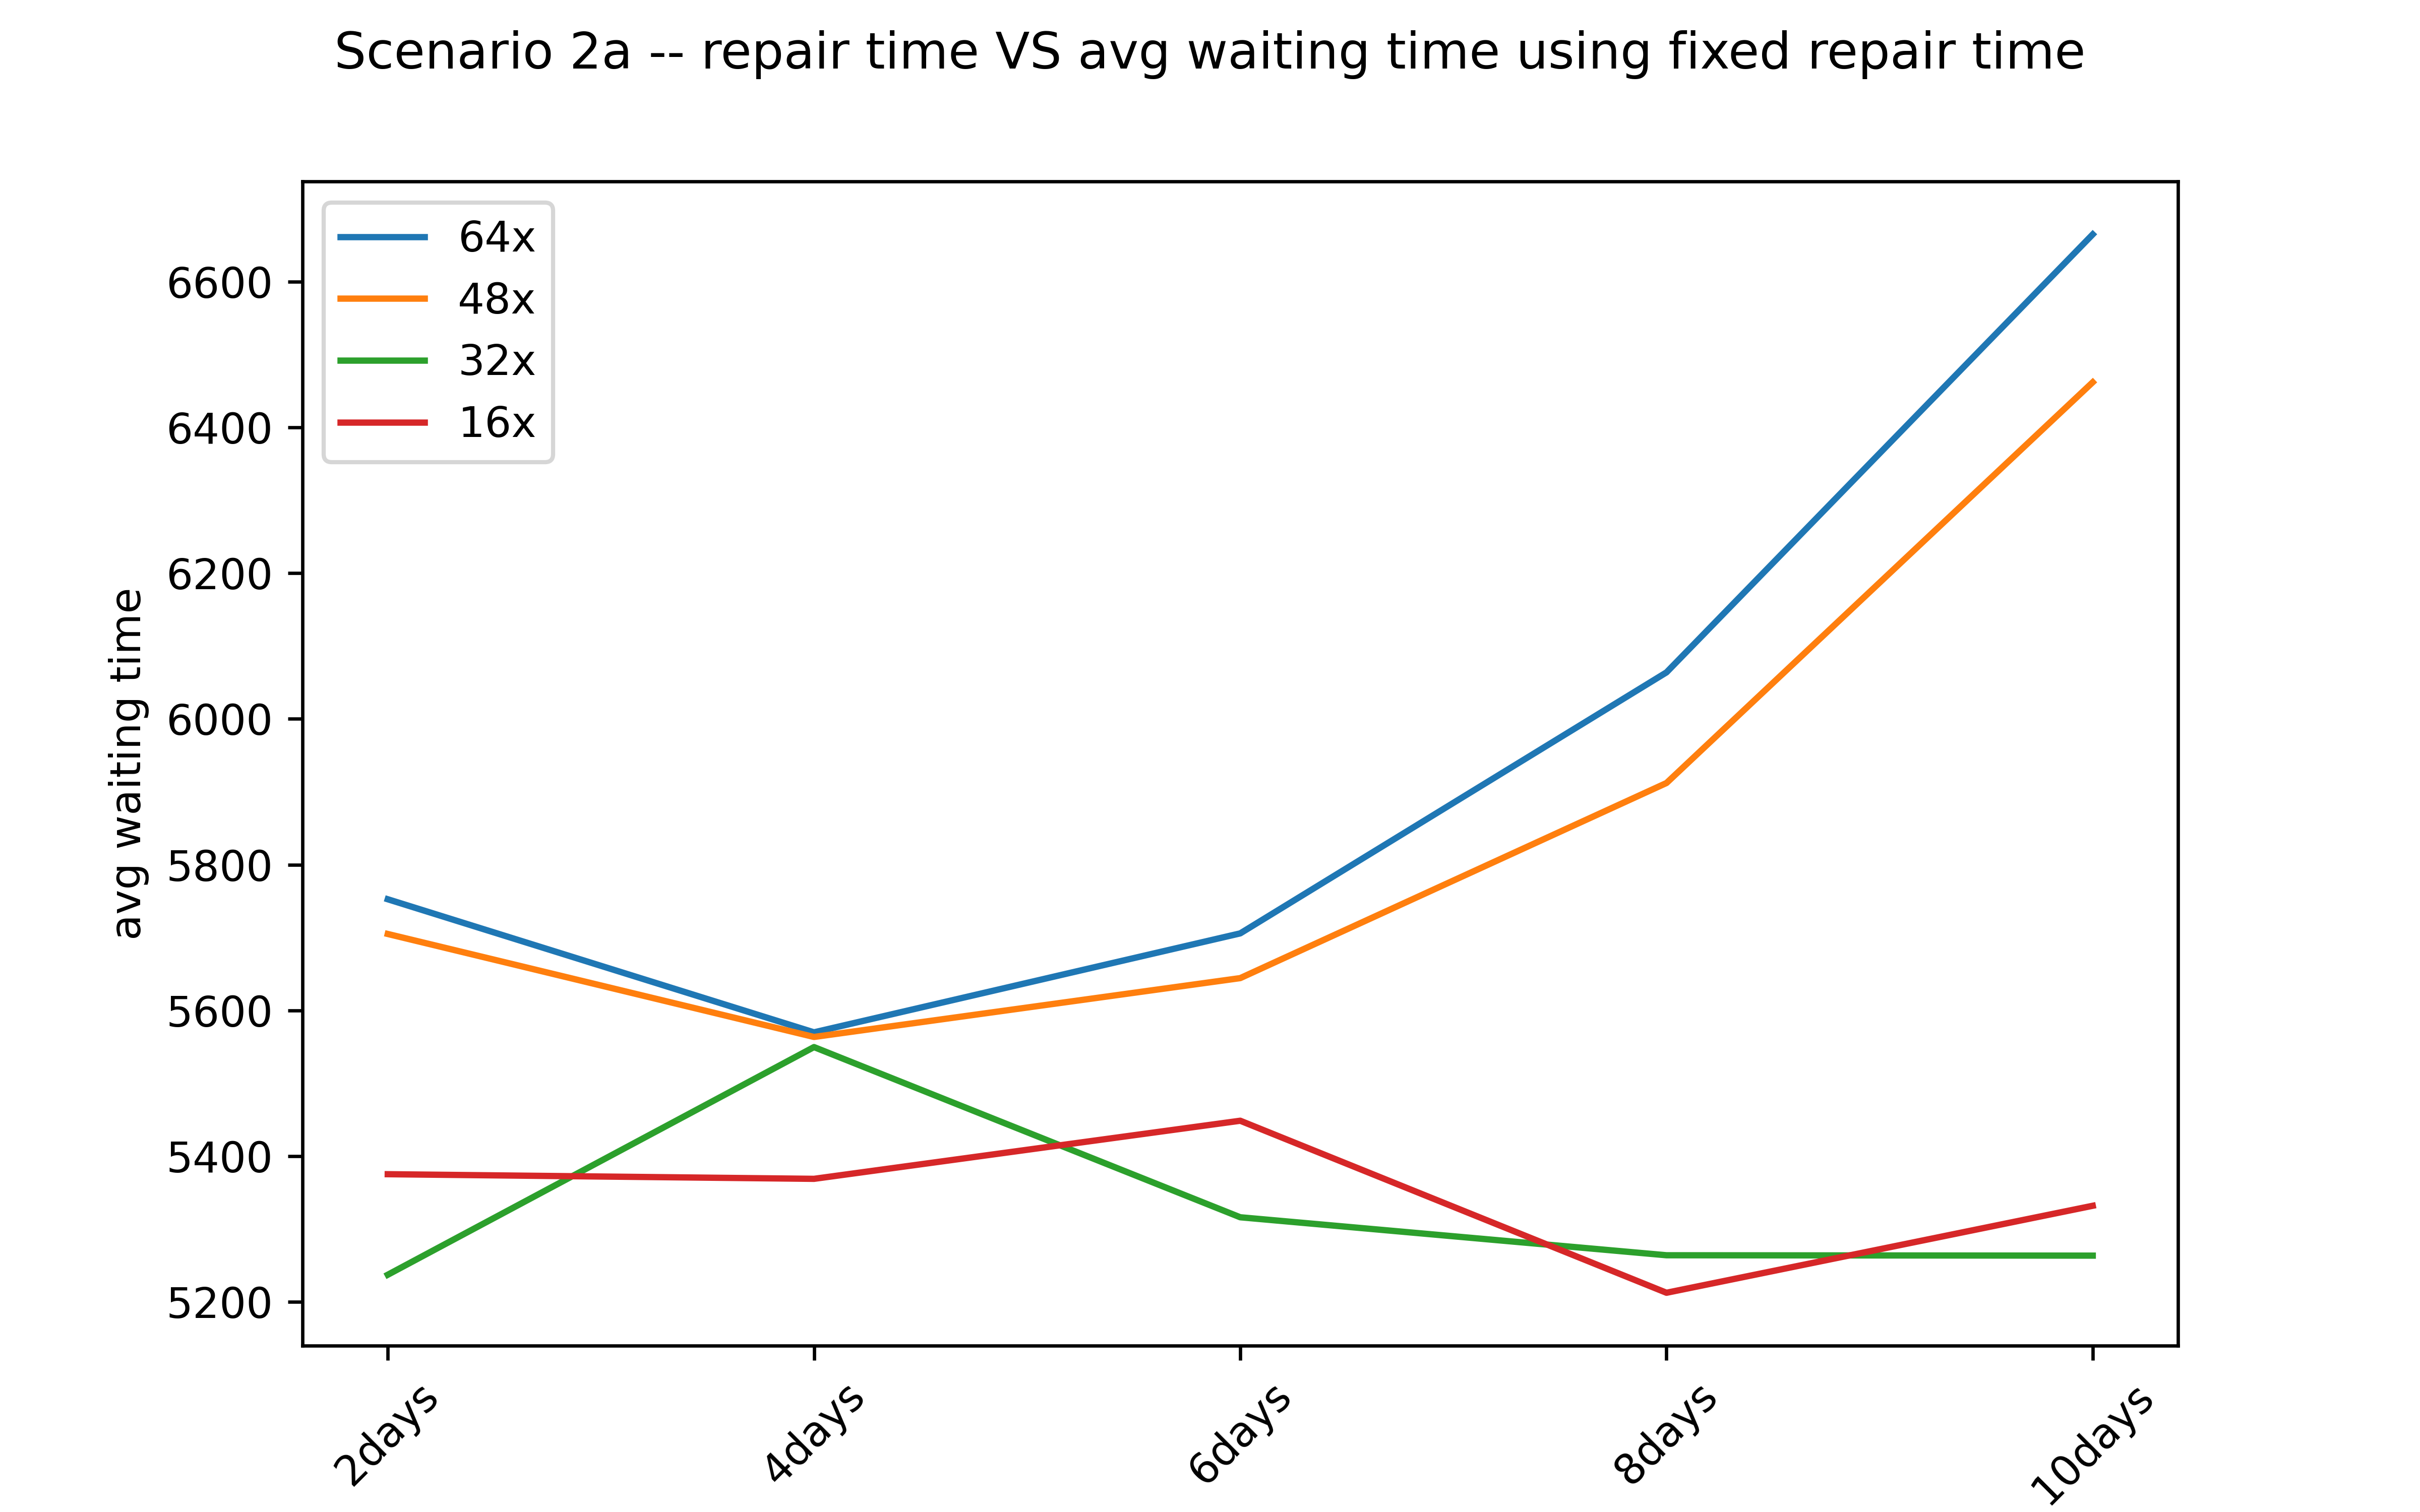
\includegraphics{./scenario_2/myplot.png}

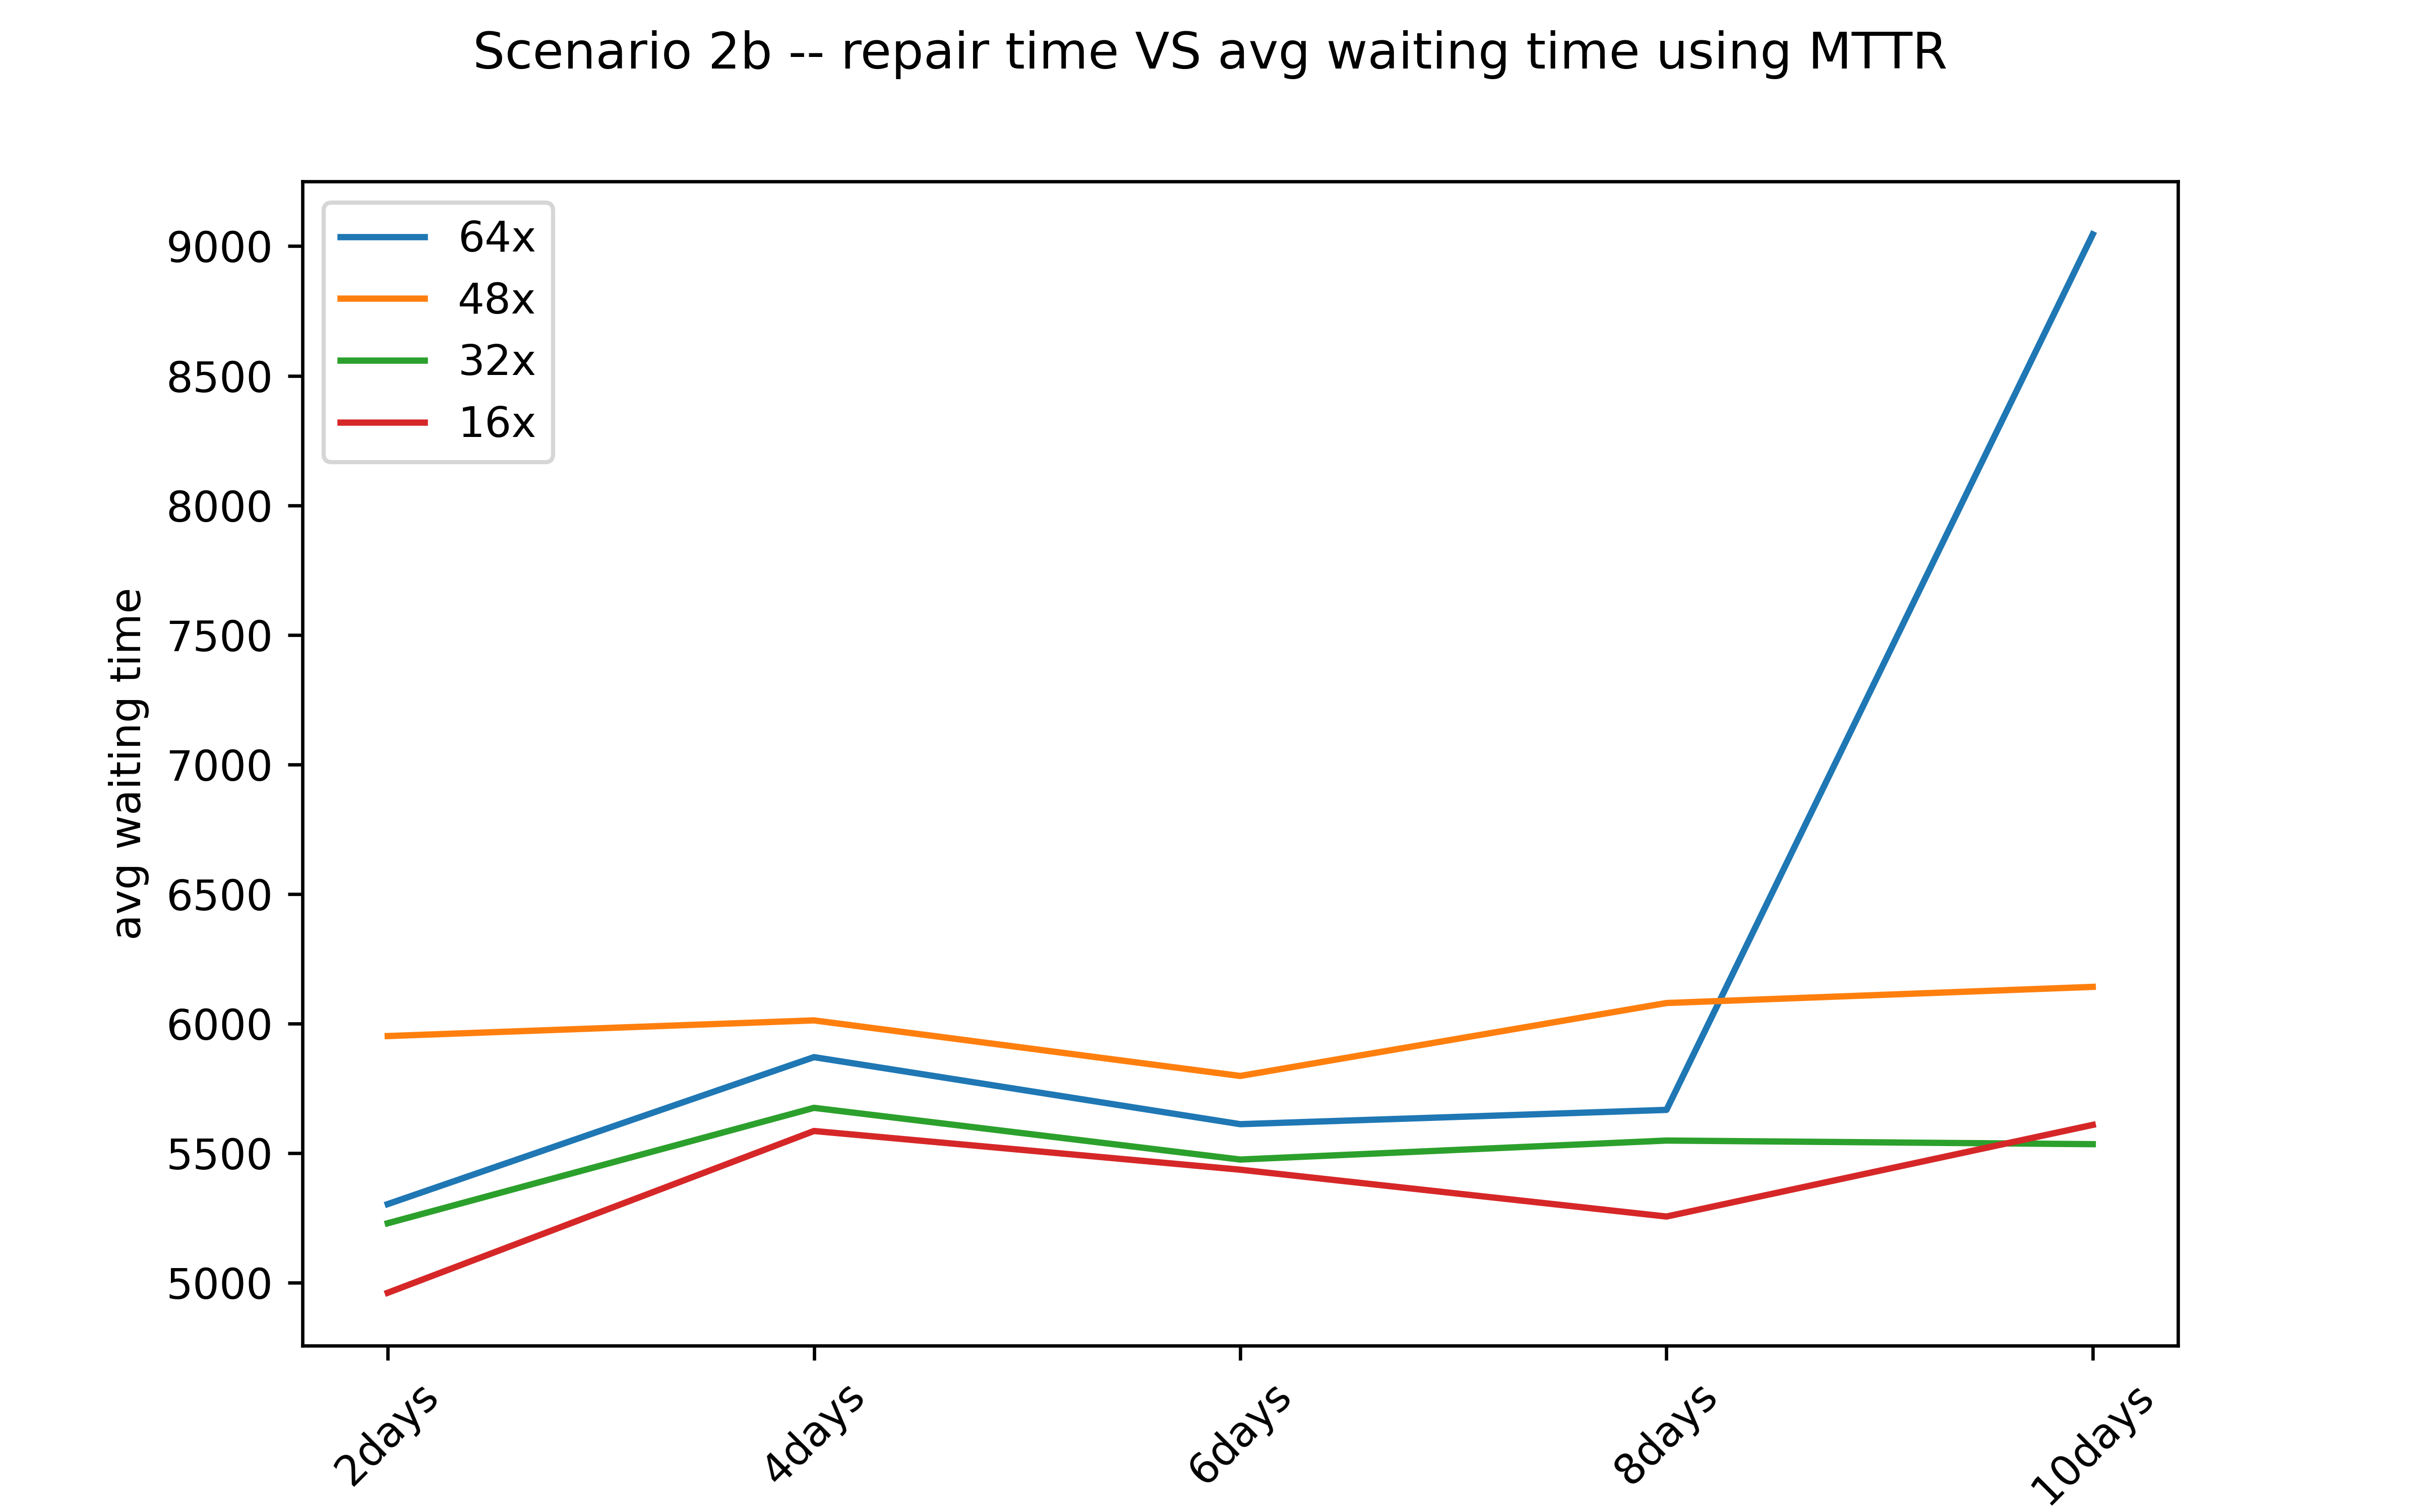
\includegraphics{./scenario_2/myplot2.png}
\end{center}

Now these graphs may not seem like much at this point.  With the variability in when failures happen and what machines they occur on, we really
need statistical information here in the form of a 'Monte Carlo' set of Runs.  Here are the same graphs with 400 runs each.

\section{Scenario 3 - Conservative Backfilling and Reservations}
\subsection{Scenario Description}
In this scenario we are going to use the conservative\_bf algorithm.  It schedules everything in the queue.  This makes it easier to add
placeholders into the schedule for "reservations" or DST's.  Unfortunately the algorithm can be quite slow.

What we want to show is using reservations and some of the analysis you can do on it.

We will use:
\begin{itemize}
  \item reservations
  \item grizzly workload
  \item output bins
\end{itemize}

The idea in this scenario is that we have a cluster the size of grizzly at 1490 nodes.  If we do weekly maintenance on the cluster,
is it better to bring the whole cluster down for some time or break parts of the cluster up through the week to do maintenance?  If 
it is better to break the cluster up, how many partitions should we do?  Lastly, we can evaluate how this impacts big jobs vs small jobs.

Scenario 3
\begin{itemize}
  \item Workload:
  \begin{itemize}
    \item grizzly 2018
    \item wallclock limit: 101\% of runtime
    \item from Feb 1, 2018  to  April 1, 2018
  \end{itemize}
  \item Reservations:
  \begin{itemize}
    \item 8 hours long reservations
    \item repeated every 7 days
    \item submitted at the start
    \item Subdivisions:1,2,4,8
    \item Subdivisions unit: 1 week
  \end{itemize}
\end{itemize}
\subsection{Make The Config File}
If you need a refresher on the format of a config file \hyperlink{general-config}{Scenario 1 covered that}.

Here we show what the config file we used looks like:

\begin{hicode}[java]
  
{
  "3a":{
          "input": {
                                      
                  "node-sweep":{
                      "range":[1490]
                      
                  },


                  "reservation-sweep":{
                          "name":"resv1",

                          "reservations-array":[
                                  {
                                      
                                          "time":"[00]:[480]:[00]",
                                          "subdivisions":"[1]",
                                          "subdivisions-unit":"[7]days [00]:[00]:[00]",
                                        
                                          "{1} subdivisions":"[2,4,8]"
                                  }
                                                                          
                          ]
                  },
                  "reservations-resv1":{
                
                        "reservations-array":[
                            {
                              "type":"parallel_homogeneous",
                              "machines":{
                                  "prefix":"a",
                                  "machine-speed":1,
                                  "total-resources":"0-1489",
                                  "interval":"0-1489"
                              },
                              "repeat-every":"7days 00:00:00",
                              "time":"09:00:00",
                              "start":"7days 12:00:00",
                              "submit":-1,
                              "count":10
                          }
                        ]
                  },
                      "batsched-policy":"conservative_bf",
                      "queue-depth":1000,
                      "grizzly-workload":{
                                          "type":"parallel_homogeneous",
                                          "machine-speed":1,
                                          "reservations":"resv1",
                                        
                                          
                                          "input":"sanitized_jobs.csv",
                                          "wallclock-limit":"101%",
                                          "time":"02-01-2018:04-01-2018"
                                                                                  
                                        }
                  },
                  "output": {
                      "avg-makespan":1,
                      "bins":"[0,2,4,8,16,32,64,128,256,512,1024,+]"
                  
                  }

          }
  }
\end{hicode}

{\large \textbf{3a}}

So on line 5 we have our node sweep, but we just use the 1490 nodes that grizzly has since we are using the grizzly workload.
Next we have the reservation sweep, but before we get into that, let's look at the reservations that the sweep acts on.  Line
26 starts the reservations, and we have called it 'resv1'.  Every \lstProperty{"reservations-<name>"} section has an array of reservation types.
In this example we just use one type of reservation, so we only define one type within the array.

We start on line 30 with the profile type \lstProperty{"type":"parallel_homogeneous"}.  The thing about using \lstProperty{"type":"parallel_homogeneous"}
is that the reservation could speed up or slow down depending on if the flops/sec sped up on the machines or slowed down.  If we used \lstProperty{"type":"delay"}
then it would be a strictly time sensitive reservation.

Next, on line 31 we define the machines this reservation type affects.  On line 34 we say that the total resources available for this reservation type is the whole cluster.
Defining this can be useful if we are doing some random machine intervals.  But in this example we are just doing a simple interval of the whole cluster.

On line 39 we set when we want this reservation type to start.  So at 7 days and 12 hours after the first job, we have a reservation.  The duration of that reservation
is set for 9 hours on line 38. On line 37 we tell it to repeat the reservation every 7 days.  On line 40 we say we want all of the reservations to submit at the start.
This means the reservation is not going to come in and kill jobs because the reservation is already there and nothing should have been scheduled on it to begin with.
There may be cases when you want to say how far in advance a reservation is scheduled before its start time.

On line 41 we have a clunky property named \lstProperty{"count"}.  This requires you to keep up with the amount of simulated time your simulation takes, as well as how many reservations
you need to have to last that simulated time.  I am doing 2 months of jobs and the reservations happen every week.  There are about 4 weeks in a month so that would mean I need at least 8 reservations.
I give it 2 extra just to make sure.  There really isn't too much problem with going over.  It can inflate your makespan, however, if you were using that as a metric.
The reason we need this property is in how reservations are made.  They are part of the workload and operate much like a job, so they are made in advance, and if you are
using things like failures, there isn't much way of knowing how long a simulation is going to run.  So you must use your best judgement.

So now that we described the reservation type, let's go over the sweep of it.  On line 12 we set the name
of the type that this sweep applies to.  We then make an array of sweeps.  Each sweep applies to the corresponding
type in the resv1 reservations-array definition.

Ok, so our base modifications are done on lines 17-19.  On line 17 we set just one duration of 8 hours (480 minutes).  This
will overwrite the 9 hours we had set.  So setting it in our type definition was not needed.
On line 18 we start with 1 subdivision.  That subdivision is going to be spread over 7 days.  Since
we start with 1 subdivision the unit of time is moot in that case.

Then on line 21 we add in a multiplier.  It is going to use the 480 minute duration and the 7 day unit, but 
it is going to change the subdivisions to 2,4,and 8.  This is going to result in 3 more jobs and therefore 3 more simulations for
a total of 4.

On line 45 we tell it we want the \lstProperty{"conservative_bf"} algorithm. On line 46 we use a queue-depth of 1,000.  This will prevent the algorithm from
taking so long, however, it can cut back on accuracy if what you wanted to simulate was a scheduler that scheduled everything in the queue in advance.  In our scenario
we tell it to quit after taking the first 1,000 jobs in the queue.

You've seen the grizzly workload before, but on line 50 we set which reservations we are using for this workload.
Also, on line 55 we set the time from February 1 until April 1, so two months.

Everything else is the same except line 61.  Here we tell our post-processing that we not only want a makespan.csv for the total summary
of our simulation, but we also want a summary for the specified bins.  The bins are operating on the amount of nodes the jobs requested.  So
we will have a summary for jobs that requested (0-2] nodes, a summary for (2-4] nodes etc... until we get to the '+'.  This says 'anything above' the previous number: 1024.
You can use a '-' at the beginning to specify 'below the next value', as well.

The binned summaries will be in your \lstFolder{expe-out/bins} folder.


\subsection{Run The Config File}
After setting \${file1} there isn't anything different in this command except the output folder:

\begin{termESC}
+?{batprompt}+ myBatchTasks.sh -f ${file1} -o scenario_3_3_bins -m bare-metal -p tasks -t 8 -s 40001  
\end{termESC}

\subsection{While Running The Sims}
You can go ahead and use the \lstTerm{progress.sh} tool as you see fit.  You will notice that
you can see the 'schedule' components in this scenario.  This is because conservative\_bf uses the
schedule class.  You may also notice the speed of jobs completing can go up and down based on the queue size.

\subsection{Aggregating Results}
So now we can aggregate the results as normal.
\begin{termESC}
+?{batprompt}+ cd ${prefix}/experiments/scenario_3_3_bins
+?{batprompt}+ aggregate_makespan.py -i $(pwd)
\end{termESC}
\subsection{Analysis}
Currently \lstFolder{total_makespan.csv} has the following header:

\csvreader[ %
tabular=|m{2.5cm}|m{2.5cm}|m{2.5cm}|m{2.5cm}|m{4cm}|m{3cm}|,
table head=\hline ,
late after line=\\\hline ]{tmh.csv}{}{\csvlinetotablerow}

and the individual binned makespan csv files in the \lstFolder{expe-out/bins} folder have the following header:

\csvreader[ %
tabular=|m{2.5cm}|m{2.5cm}|m{2.5cm}|m{2.5cm}|m{4cm}|m{3cm}|,
table head=\hline ,
late after line=\\\hline ]{bmh.csv}{}{\csvlinetotablerow}

both of which allow for this code:

\begin{hicode}[python]
  import pandas as pd
  import numpy as np
  import matplotlib.pyplot as plt
  import seaborn as sns
  import pathlib
  import os

  # a function that is in the .../basefiles/functions.py module
  # it takes a project path, a function that you want to apply to each simulation,
  # and the starting arguments that will be passed to the passed function
  def traverse_project_folder(path,myFunc,inputArgs):
      experiments=[i for i in os.listdir(path) if os.path.isdir(path+"/"+i)]
      for exp in experiments:
          jobs=[i for i in os.listdir(f"{path}/{exp}") if \
            os.path.isdir(f"{path}/{exp}/{i}")]
          for job in jobs:
              ids=[i for i in os.listdir(f"{path}/{exp}/{job}") if \
                os.path.isdir(f"{path}/{exp}/{job}/{i}")]
              for ourId in ids:
                  runs=[i for i in os.listdir(f"{path}/{exp}/{job}/{ourId}") if \
                    os.path.isdir(f"{path}/{exp}/{job}/{ourId}/{i}")]
                  for run in runs:
                      current_run=f"{path}/{exp}/{job}/{ourId}/{run}"
                      pathArgs={"experiments":experiments,"jobs":jobs,"ids":ids,\
                        "runs":runs,"path":path,"exp":exp,"job":job,"ourId":ourId,\
                        "run":run,"current_run":current_run}
                      inputArgs=myFunc(pathArgs,inputArgs)
  
      return inputArgs
  
  # this is the function that I want to be run on each sim folder
  # it requires that pathArgs and inputArgs be passed into it

  # this particular function will gather all the avg_waiting times from each binned
  # makespan summary.
  def myFunc(pathArgs,inputArgs):
      if inputArgs["first"]==True:
          bin_files=[i for i in os.listdir(f"{pathArgs['current_run']}/output/expe-out/bins") \
            if os.path.splitext(i)[1] == ".csv"]
          bins=[os.path.splitext(i)[0].split("_")[1:] for i in bin_files]
          starts=[]
          ends=[]
          avg_waitings={}
          avg_waiting=[]
          for ourBin in bins:
              starts.append(ourBin[0])
              ends.append(ourBin[1])
              file=f"{ourBin[0]}_{ourBin[1]}.csv"
              df = pd.read_csv(\
                f"{pathArgs['current_run']}/output/expe-out/bins/makespan_{file}",\
                sep=",",header=0)
              avg_waiting=df["avg_waiting"].values[0]
              avg_waitings[f"{ourBin[0]}_{ourBin[1]}"]=[avg_waiting]
      else:
          bin_files=inputArgs["bin_files"]
          bins=inputArgs["bins"]
          starts=inputArgs["starts"]
          ends=inputArgs["ends"]
          avg_waitings=inputArgs["avg_waitings"]
          for ourBin in inputArgs["bins"]:
              file=f"{ourBin[0]}_{ourBin[1]}.csv"
              df = pd.read_csv(\
                f"{pathArgs['current_run']}/output/expe-out/bins/makespan_{file}",\
                sep=",",header=0)
              avg_waiting=df["avg_waiting"].values[0]
              avg_waitings[f"{ourBin[0]}_{ourBin[1]}"].append(avg_waiting)
      inputArgs={"bin_files":bin_files,"bins":bins,"starts":starts,"ends":ends,\
       "avg_waitings":avg_waitings,"first":False}
      return inputArgs
  
  
  
  
  scriptPath = str(pathlib.Path(__file__).parent.absolute())
  width=10
  height=10
  BASE_SECONDS = 1728000000  #not used in this scenario
  
  fig, axs = plt.subplots(1, 1, figsize=(width, height))
  
  df = pd.read_csv("./total_makespan.csv",header=0,sep=",")
  
  #1 subdivision  is 'job':experiment_1
  #2 subdivisions is 'job':experiment_2 
  #4 subdivisions is 'job':experiment_3
  #8 subdivisions is 'job':experiment_4

  # First we graph an overall summary of the amount of Subdivisions vs
  # the avg waiting time

  # unfortunately much of the info of the reservations used is not in any summary
  # you can find the reservation info used for this sim in the Run_#/input/config.ini file

  # we get the experiment num and use that to determine how many subdivisions this sim had
  experiments=df.job.str.extract(r'experiment_(?P<experiment>\d+)')
  experiments["experiment"]=experiments.experiment.astype(int)
  df = pd.concat([df,experiments],axis=1)
  df["subdivisions"]=2**(df["experiment"]-1)
  
  # we plot the subdivisions vs avg_waiting
  plt.plot(df["subdivisions"],df["avg_waiting"])
  axs.set_xlabel("subdivisions")
  axs.set_ylabel("avg waiting time")
  axs.set_xticks([1,2,4,8])
  
  axs.set_title("Scenario 3a -- Subdivisions vs Avg Waiting Time")
  fig.savefig("myplot.png",dpi=600)
  
  
  # we are then going to graph the binned avg waiting times

  fig, axs = plt.subplots(1, 1, figsize=(width, height))
  
  # we get the hsv color map 
  cmap = plt.get_cmap('hsv')
  # we then evenly space the colors out.  I don't want the redish ones at the end
  # of the color map looking like the red ones at the beginning of the color map
  # so I do a linspace of 0 to only .75.  I want 11 colors in that range for the
  # 11 bins.
  colors = cmap(np.linspace(0,.75,11))
  
  # I traverse the project folder and apply my 'myFunc' function
  inputArgs={"first":True}
  inputArgs = traverse_project_folder(scriptPath,myFunc,inputArgs)
  
  # I plot the graphs each with a different color
  count=0
  for ourBin in inputArgs["bins"]:
      avg_waiting=inputArgs["avg_waitings"][f"{ourBin[0]}_{ourBin[1]}"]
      plt.plot([1,2,4,8],avg_waiting,color=colors[count],label=f"({ourBin[0]},{ourBin[1]}]")
      count+=1
  
  plt.legend(loc="lower right",bbox_to_anchor=(1.2,0.0))
  axs.set_xlabel("subdivisions")
  axs.set_ylabel("avg waiting time")
  
  axs.set_title("Scenario 3a -- Subdivisions vs Avg Waiting Time By Bin")
  axs.set_xticks([1,2,4,8])
  fig.savefig("myplot2.png",dpi=600, bbox_inches='tight')
  
  

# Now I want to normalize the plots.  Each line is normalized to where
# they started at 1 subdivision.


  fig, axs = plt.subplots(1, 1, figsize=(width, height))
  count=0
  for ourBin in inputArgs["bins"]:
      avg_waiting=inputArgs["avg_waitings"][f"{ourBin[0]}_{ourBin[1]}"]

      # here is where things get normalized
      avg_waiting=avg_waiting/avg_waiting[0]
      
      plt.plot([1,2,4,8],avg_waiting,color=colors[count],label=f"({ourBin[0]},{ourBin[1]}]")
      count+=1
  
  plt.legend(loc="lower right",bbox_to_anchor=(1.2,0.0))
  axs.set_xlabel("subdivisions")
  axs.set_ylabel("avg waiting time normalized")
  
  axs.set_title("Scenario 3a -- Subdivisions vs Avg Waiting Time By Bin Normalized")
  axs.set_xticks([1,2,4,8])
  fig.savefig("myplot3.png",dpi=600, bbox_inches='tight')
  
  
\end{hicode}

And here are the results:
\begin{center}
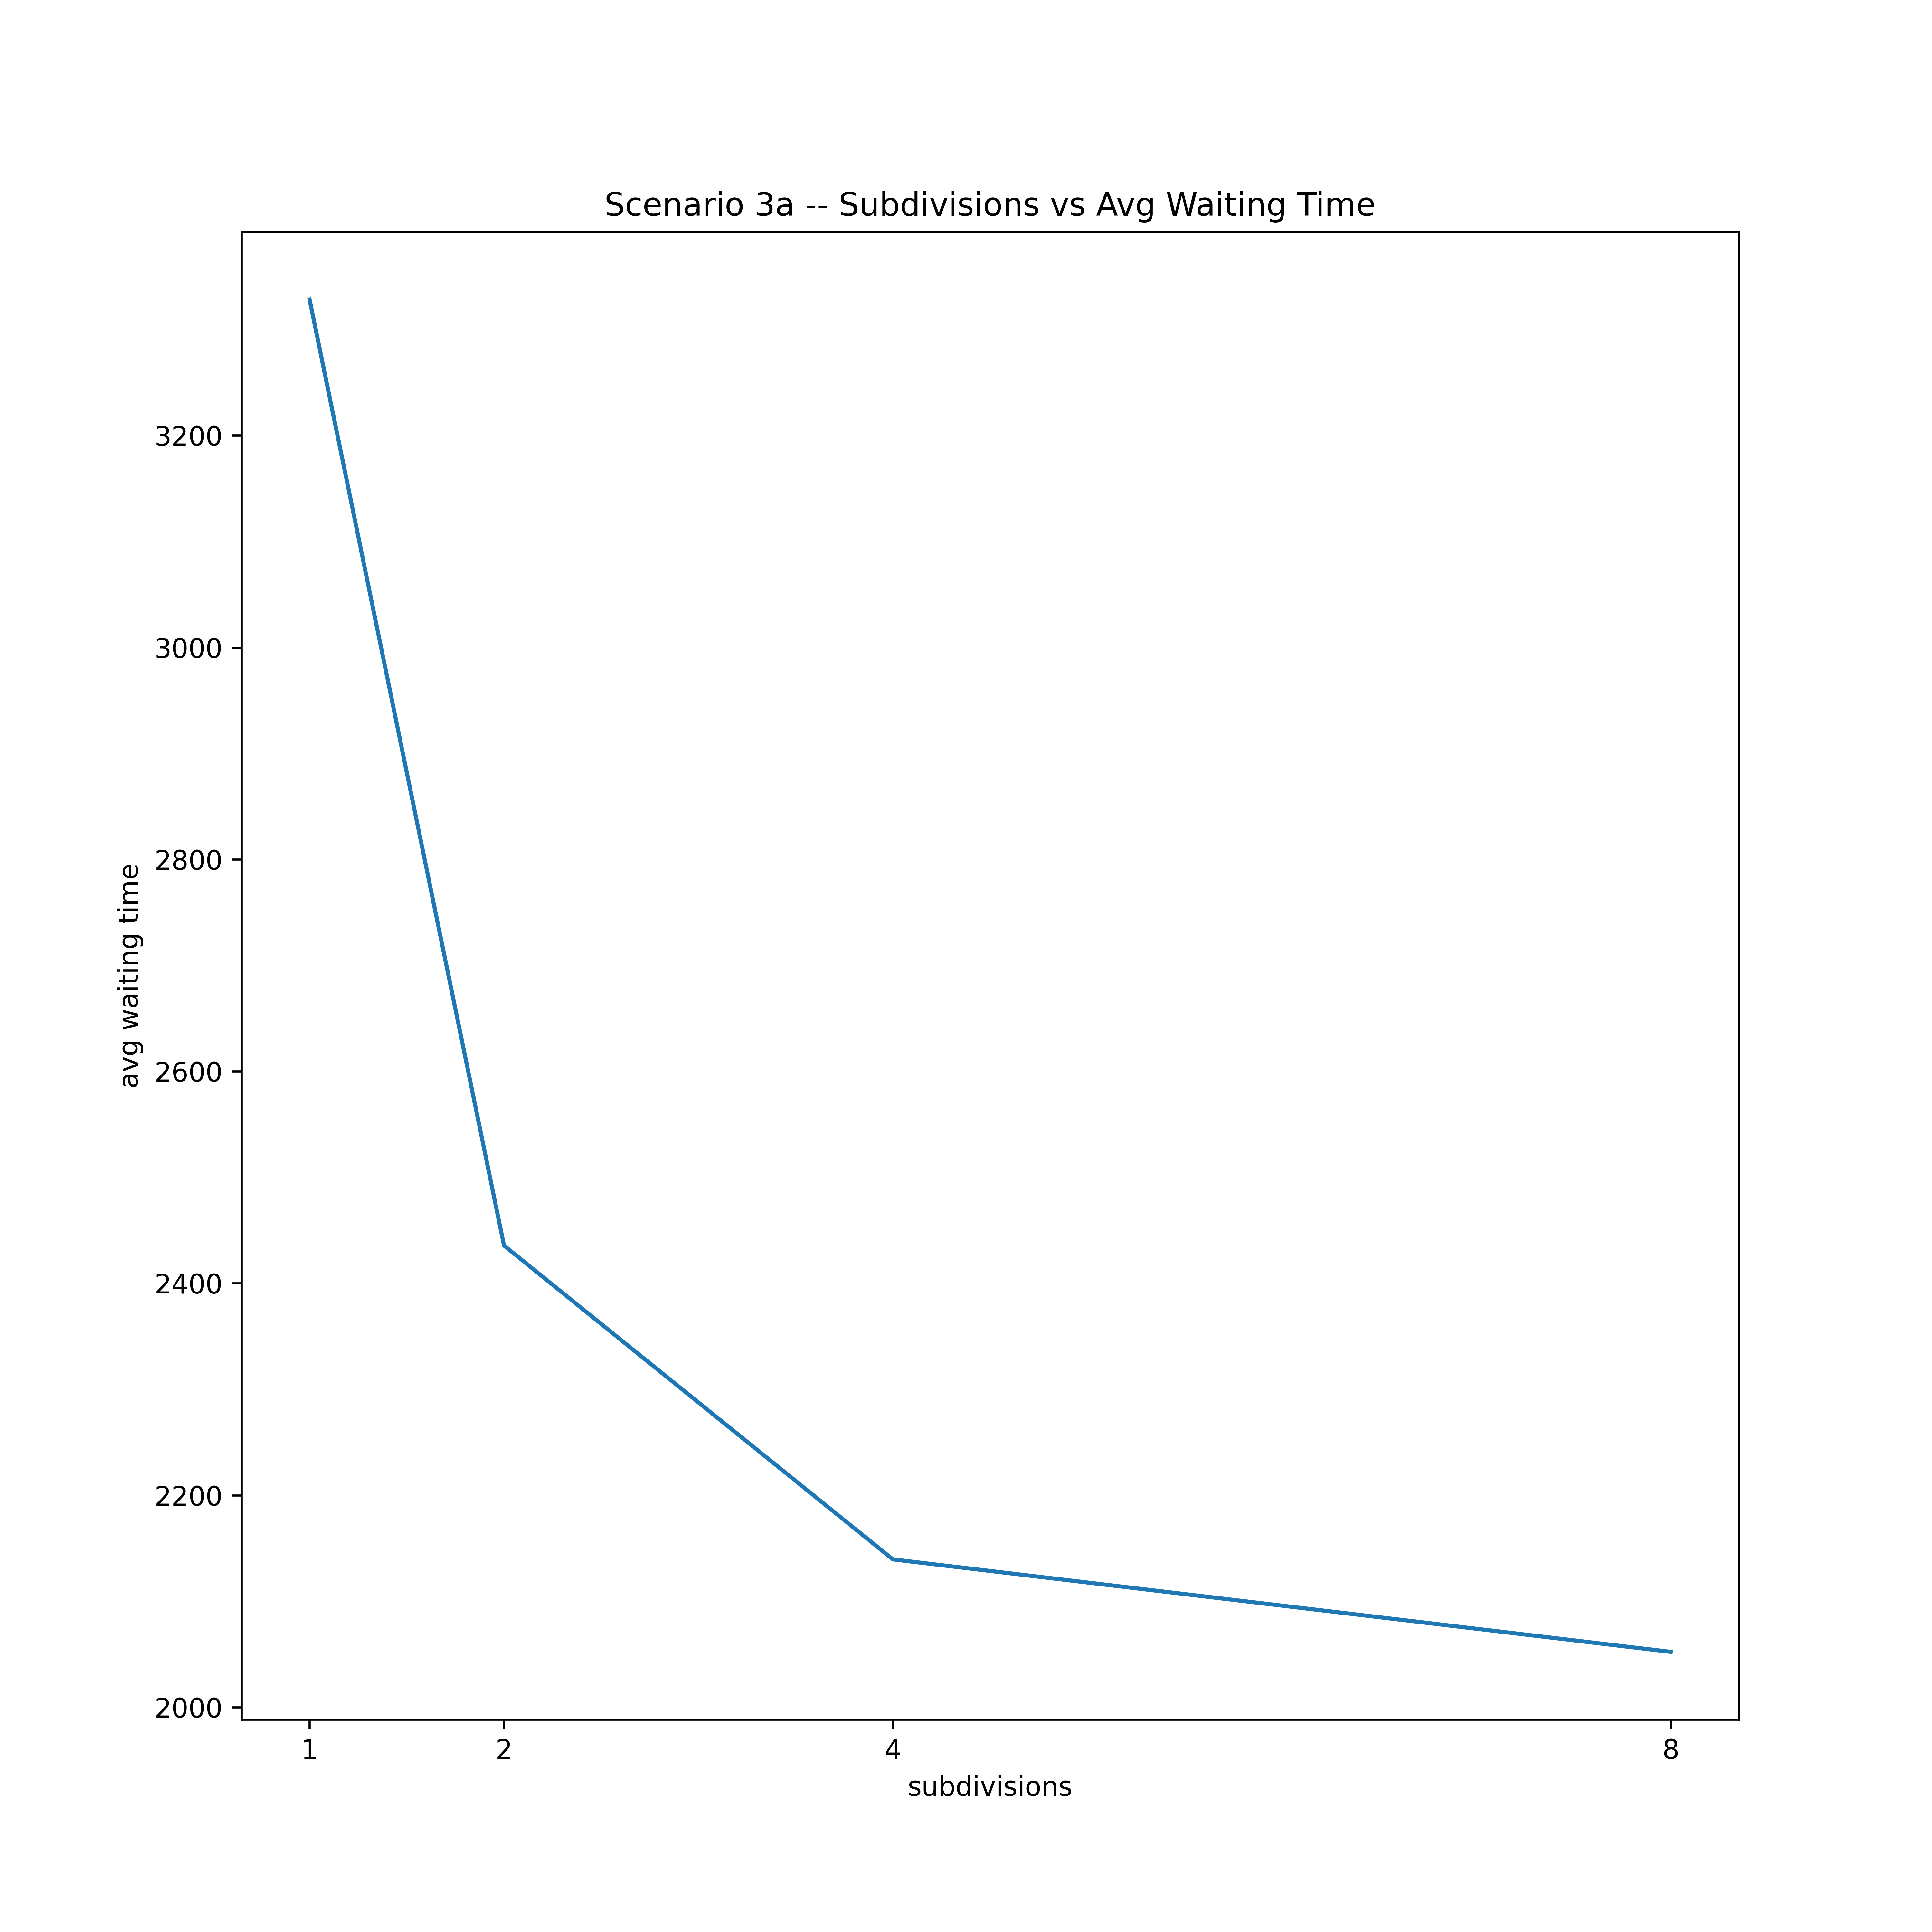
\includegraphics[scale=.5]{./scenario_3/myplot.png}
\end{center}

As you can see, there is a tremendous benefit to splitting the cluster up into 8
subdivisions, but the trend is that the improvement is diminishing.  Breaking it up into
16 probably isn't so advantageous.

Keep in mind, this is a simulation with very specific dials set.  Things would change
a bit with a different reservation duration, subdivision unit time, etc...
\begin{center}
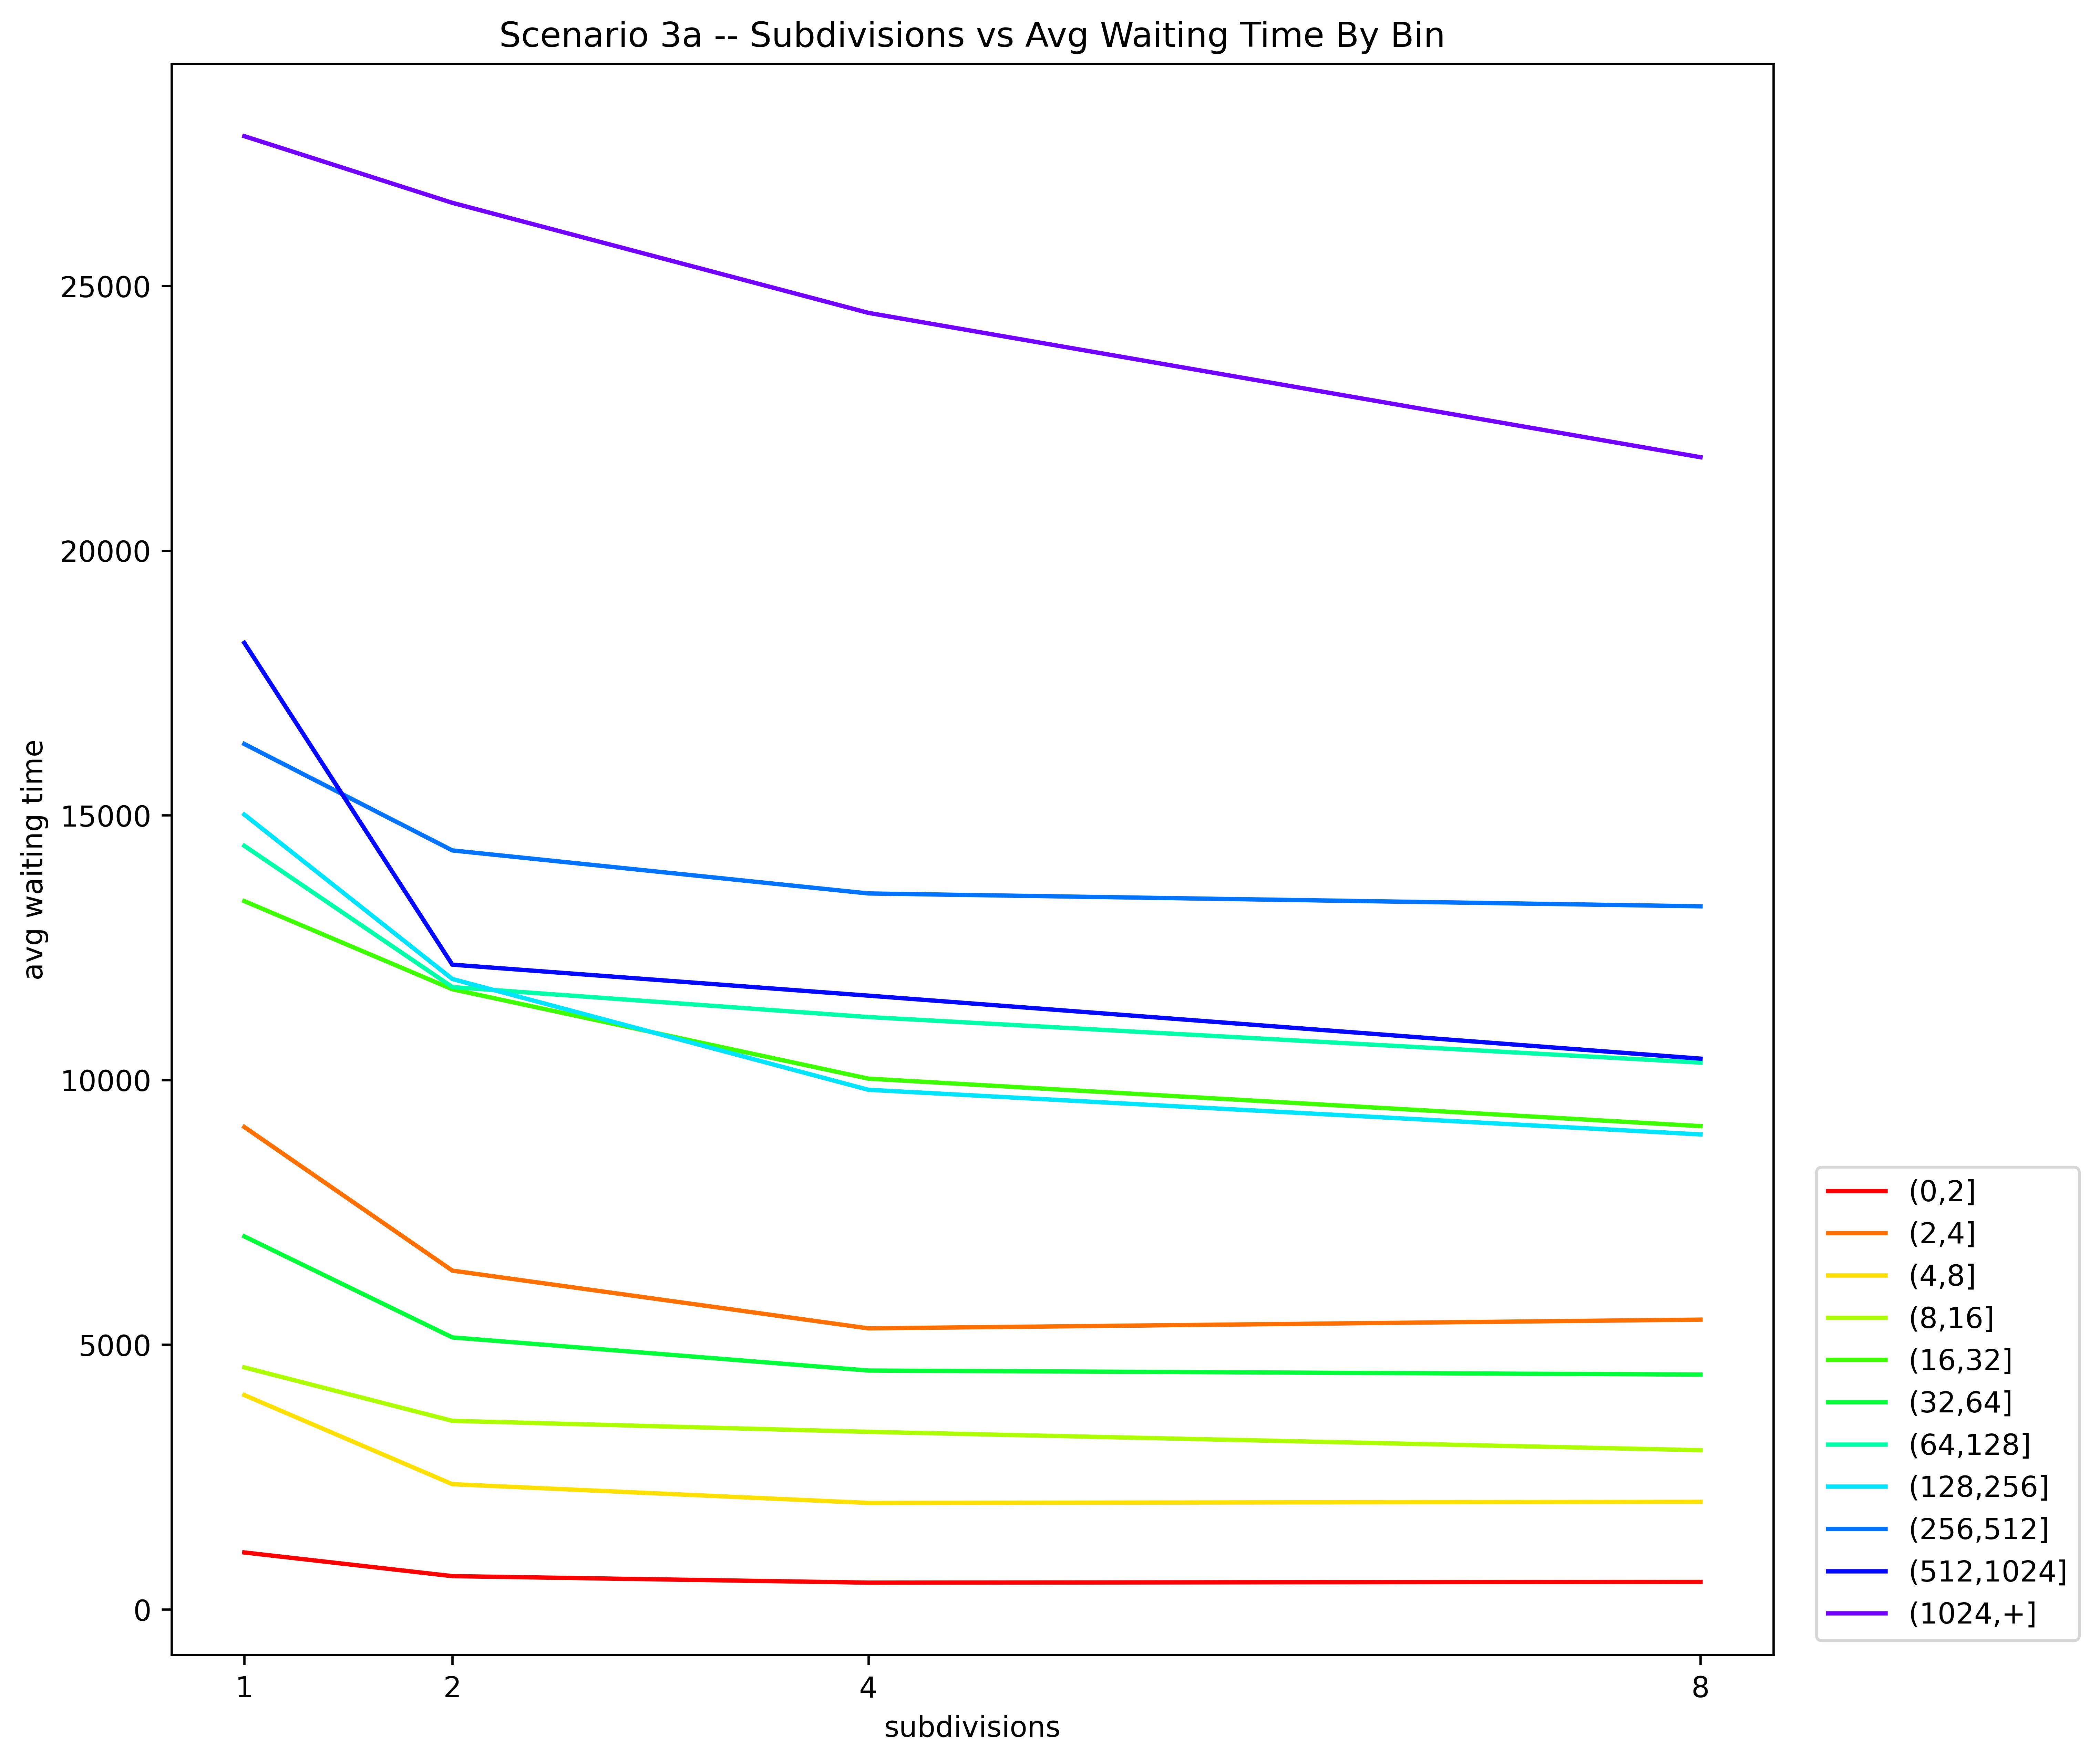
\includegraphics[scale=.5]{./scenario_3/myplot2.png}
\end{center}

Here it looks like the largest jobs do the best with breaking the cluster up and the smallest
jobs don't see much improvement at all.

\begin{center}
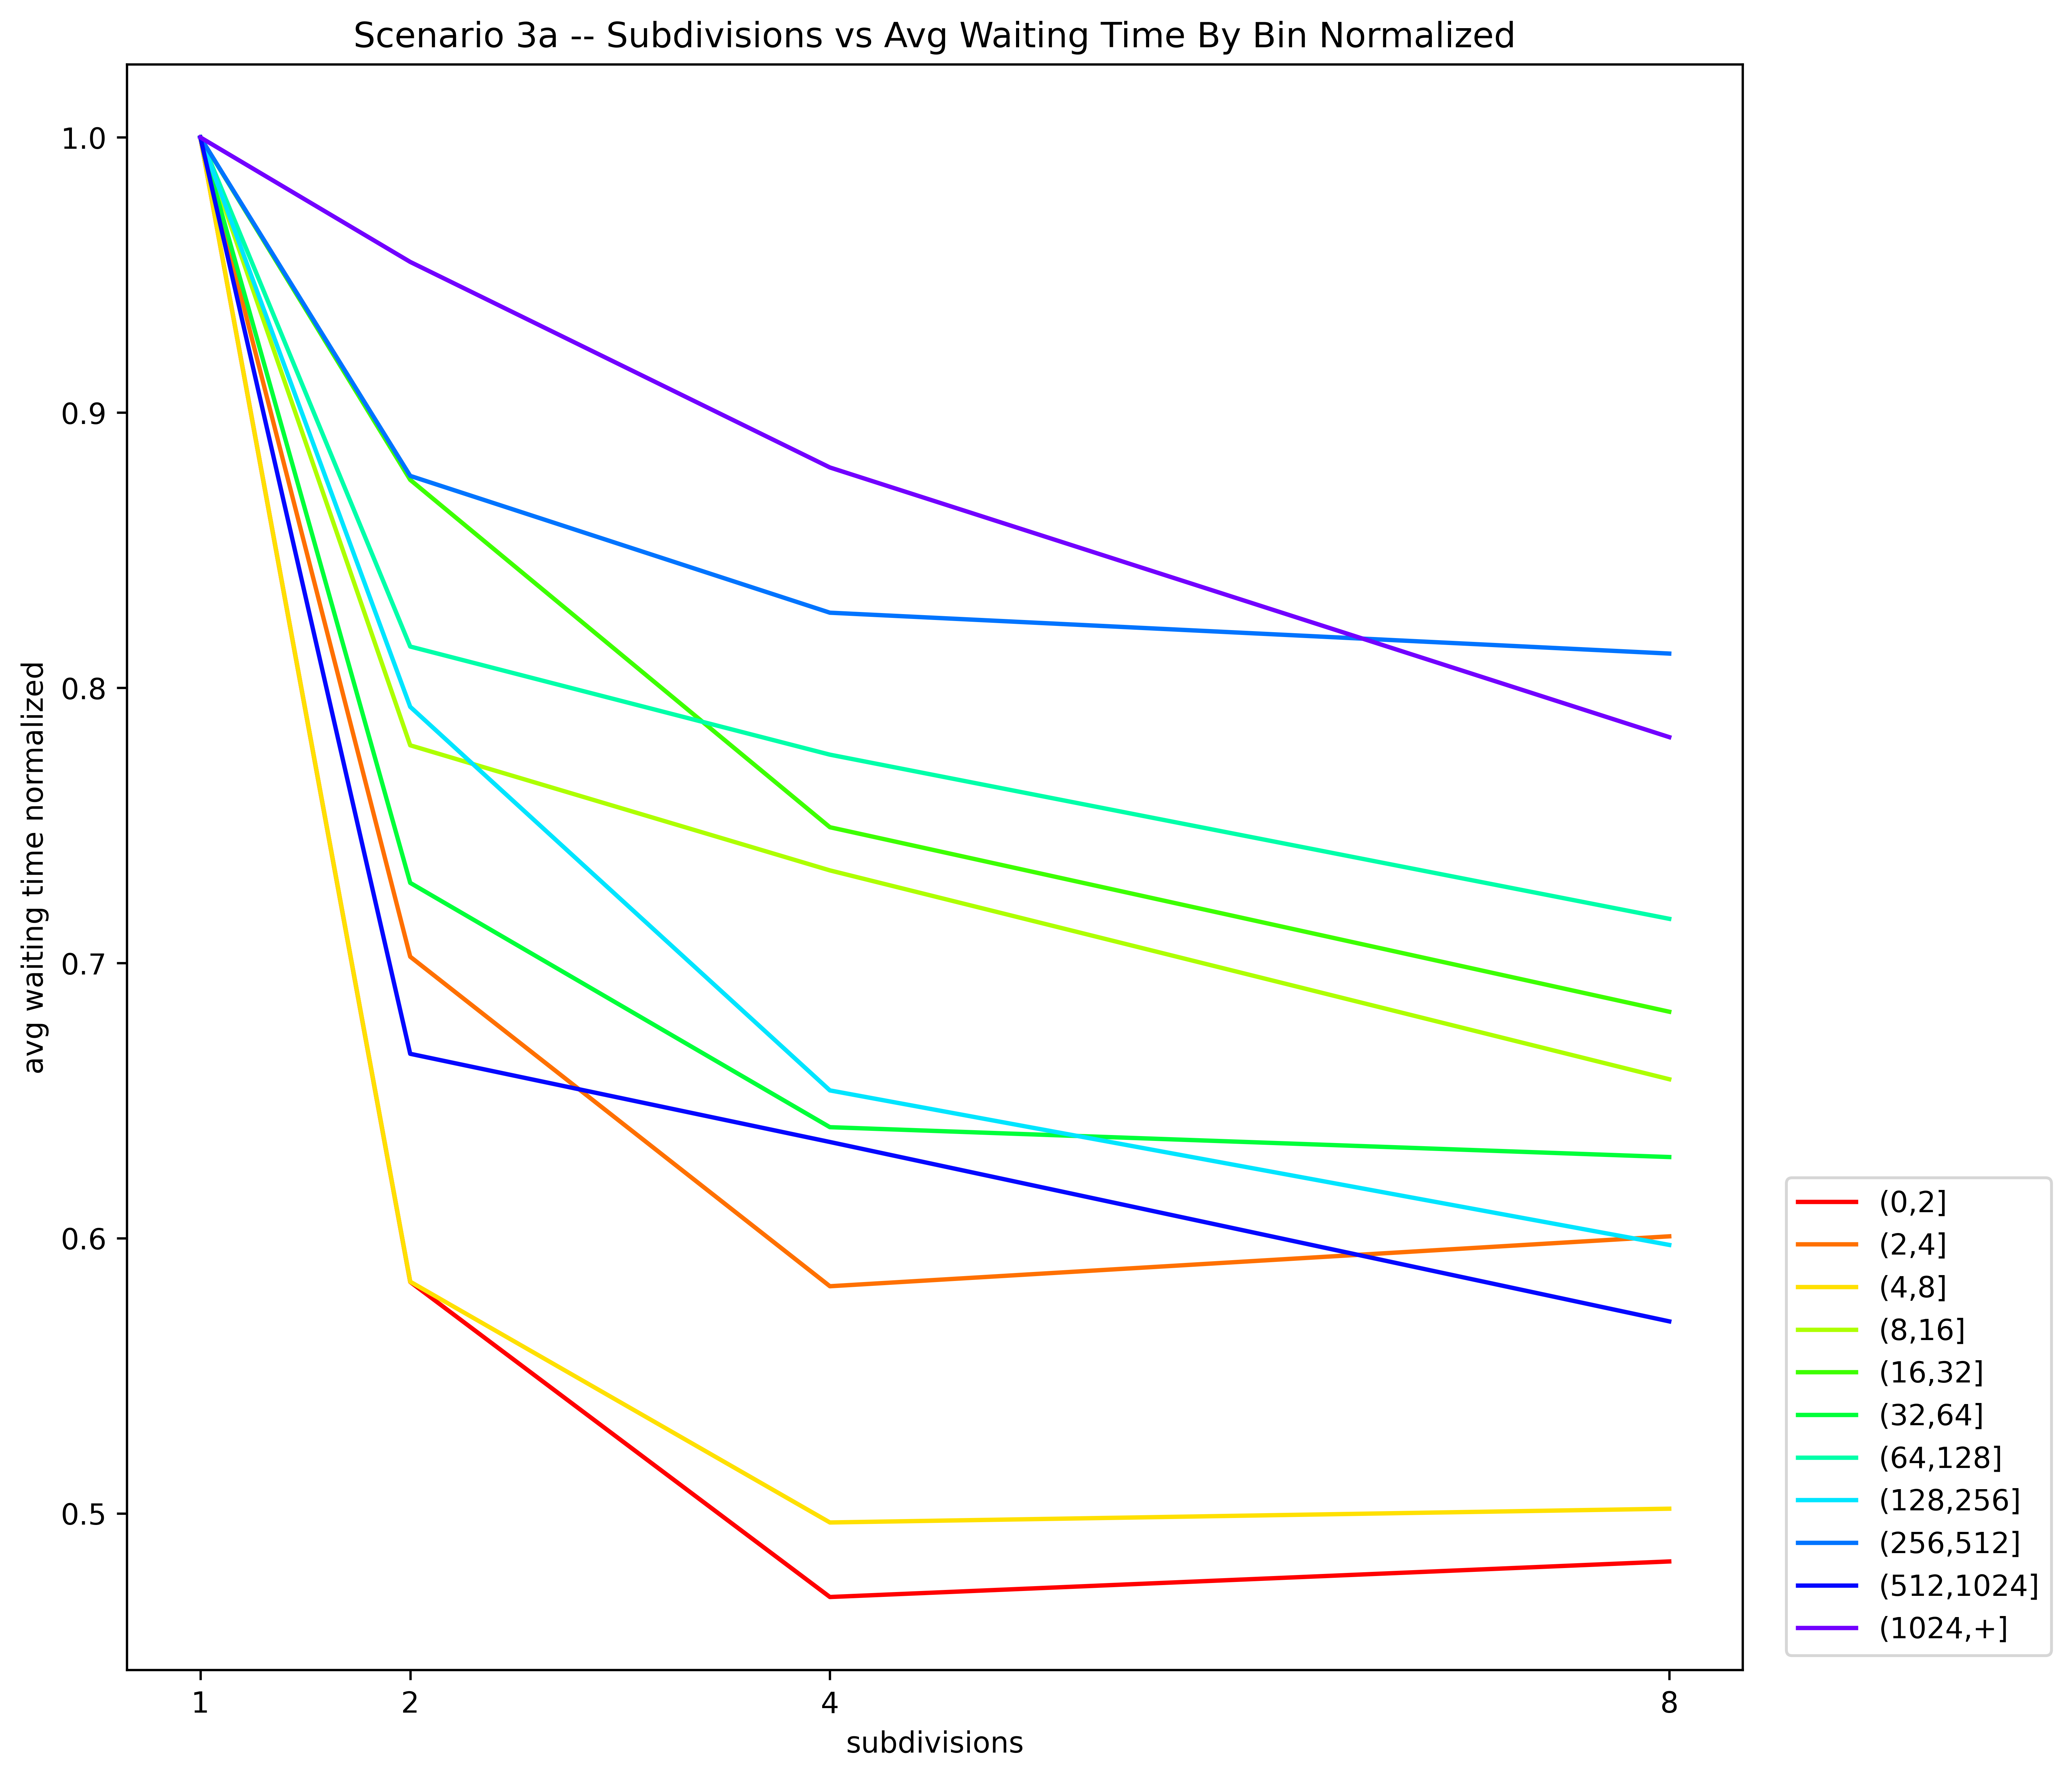
\includegraphics[scale=.5]{./scenario_3/myplot3.png}
\end{center}

Here you can see that, actually, small jobs see a huge improvement in avg waiting time when going from
1 subdivision to 2 and to 4.
You can also see that compared to not partitioning the maintenance up at all, a subdivision of 8 can
have about a 20\% difference in average waiting time for the largest jobs.



\end{document}